\documentclass[12pt,a4paper,oneside]{book}

\usepackage{kotex}
\usepackage[pdftex]{graphicx}
\usepackage{epstopdf}
\usepackage{amsthm}
\usepackage{amsmath}
\usepackage{multirow}
\usepackage{amssymb}
\pagestyle{plain}



% MATH  ------------------------------------------------------------------

\newcommand{\spart}[1]{\left(#1\right)}
\newcommand{\ppart}[1]{\left[#1\right]}
\newcommand{\norm}[1]{\left|#1\right|}
\newcommand{\med}{\mathrm{median}}
\newcommand {\bm}[1]{\mbox{\boldmath{$#1$}}}
\newcommand {\bb} {{\bm{\beta}}}
\newcommand {\argmin} {\mathop{\rm{argmin}}}

% Line spacing -----------------------------------------------------------
\newlength{\defbaselineskip}
\setlength{\defbaselineskip}{\baselineskip}
\newcommand{\setlinespacing}[1]%
           {\setlength{\baselineskip}{#1 \defbaselineskip}}
\newcommand{\doublespacing}{\setlength{\baselineskip}%
                           {2.0 \defbaselineskip}}
\newcommand{\singlespacing}{\setlength{\baselineskip}{\defbaselineskip}}


%\setlength{\tclineskip}{1.66\baselineskip}
\linespread{1.6}

% Graphic  -----------------------------------------------------------
\DeclareGraphicsRule{.png}{bmp}{}{}

% Bibliography ------------------------------------------------------------
\renewcommand\bibname{Bibliography}

% Table of Contents

% Theorem Style
% THEOREMS ---------------------------------------------------------------
\theoremstyle{plain}
\newtheorem{thm}{Theorem}
\newtheorem{cor}[thm]{Corollary}
\newtheorem{lem}[thm]{Lemma}
\newtheorem{prop}[thm]{Proposition}
%
\theoremstyle{definition}
\newtheorem{defn}{Definition}[chapter]
%
\theoremstyle{remark}
\newtheorem{rem}{Remark}[chapter]
%
\theoremstyle{definition}
\newtheorem{exam}{Example}[chapter]
%
\numberwithin{equation}{chapter}
%\renewcommand{\theequation}{\thesection.\arabic{equation}}
\setlength{\textwidth 140mm} \setlength{\textheight 200mm}





\begin{document}
%\iffalse
% Cover





%%%%% Cover 1
 \linespread{1.0}
 \thispagestyle{empty}
 \begin{center}
 {\Large Thesis for the Degree of Master}
 \end{center}
 \vspace{20mm}
 \begin{center}
 \LARGE A Study on Comparison of\\ Bayesian Network Structure Learning Algorithm for Selecting Appropriate Model
 \end{center}
 \vspace{20mm} 
  \begin{center}
 {\Large by}
 \end{center}
 \begin{center}
 {\Large YOO, JAE SEONG}
 \end{center}
 \vspace{40mm}
 \begin{center}
 {\Large Department of Statistics}
 \end{center}
 \begin{center}
 {\Large Graduate School}
 \end{center}
 \begin{center}
 {\Large Korea University}
 \end{center}
  \vspace{5mm}
 \begin{center}
 {\Large December, 2014}
 \end{center}
 \linespread{1.6}





\newpage{}
%%%%% Cover 2
 \linespread{1.0}
 \thispagestyle{empty}
 \vspace{15mm}
 \begin{center}
 {\Large 崔 太 連 敎授指導 \\ 碩 士 學 位 論 文
}
 \end{center}
 \vspace{20mm}
 \begin{center}
  \LARGE A Study on Comparison of\\ Bayesian Network Structure Learning Algorithm for Selecting Appropriate Model
 \end{center}
 \vspace{20mm}
 \begin{center}
 {\Large 이 論文을 統計學碩士 學位論文으로 提出함}
 \end{center}
 \vspace{15mm}
 \begin{center}
 {\Large 2014年 \quad 12月 \quad 日}
 \end{center}
 \vspace{20mm}
 \begin{center}
 {\Large 高麗大學校 大學院}
 \end{center}
	 \begin{center}
  {\Large 統 計 學 科}
 \end{center}
 \begin{center}
 {\Large 兪 \quad\quad 在 \quad\quad 成}
 \end{center}
 \linespread{1.6}





\newpage{}		
%%%%% Cover 3
 \linespread{1.0}
 \thispagestyle{empty}
 \vspace{20mm}
 \begin{center}
 {\LARGE 兪在成의 統計學碩士 學位論文 \\ 審査를 完了함}
 \end{center}
 \vspace{50mm}
 \begin{center}
{\Large 2014年 \quad 12月 \quad 日}
 \end{center}
 \vspace{55mm}
 \begin{center}
 {\Large  \underline{委員長 \hspace{60mm} (印)} \\ \vspace{7mm}
          \underline{委 \quad 員\hspace{60mm} (印)} \\ \vspace{7mm}
          \underline{委 \quad 員\hspace{60mm} (印)} \\ }
 \end{center}
 \linespread{1.6}





\newpage{}
%%%%% Abstract
    \pagenumbering{roman}
    \typeout{Abstract}

\begin{center}
{\Large 국 문 초 록}
\end{center}
\vspace{1cm} {\small \ \indent
본 논문에서는 R의 bnlearn 패키지에서 제공하는 베이지안 네트워크 구조학습 알고리즘 간의 성능을 비교하였다.

베이지안 네트워크 구조 학습 결과에 대한 성능 평가는 score를 이용하는 방법과, 목표 네트워크와 학습된 네트워크를 서로 비교하는 방법이 있다. 본 논문에서는 이 두 가지 방법으로 알고리즘별 성능을 비교했을 때, 결과가 서로 다를 수 있음을 확인하였다.

Topology에 따른 Synthetic Data를 생성, 이에 대하여 알고리즘별 성능을 비교하여, 목표 네트워크의 형태에 따라 적합한 알고리즘 선택을 할 수 있도록 객관적인 방향을 제시하고자 하였다.

그동안 베이지안 네트워크 데이터 생성기가 매우 고가이거나, 공개된 툴도 매우 사용하기 까다로웠기 때문에, 베이지안 네트워크 관련 실증 연구는 사례 데이터를 이용한 경우가 대부분이었다. 이에 따라 Bayesian Network 모델을 바탕으로 R에서 데이터를 생성할 수 있는 생성기를 제작하여 공개하였다.
}



\newpage{}
%%%%% Abstract
    \pagenumbering{roman}
    \typeout{Abstract}

\begin{center}
{\Large Abstract}
\end{center}
\vspace{1cm} {\small \ \indent
In this paper, we compare the performance between the Bayesian network structure learning algorithm provided by \textbf{bnlearn} package in \textbf{R}.

The performance of the study results is evaluated by using a score method comparing between the target network and the learning network. In this paper, it was confirmed that algorithm specific performance test results using fore-mentioned methods are different.

Unlike most previous studies which generally used real data, synthetic data generated based on topology was used to compare performance of contrast-specific algorithm. The aim of this paper is to provide objective guidance of selecting suitable algorithm in accordance to target network.

Previous tools suffer from serious trade-off between cost and complexity, restricting most studies relevant to Bayesian network to using only real data. To address such problem, a data generator based on Bayesian network model using \textbf{R} is built and introduced.
} 
%\addtocounter{page}{-1}
 \tableofcontents
 \newpage
 \listoftables
 \newpage
 \listoffigures
%\fi

\newpage

\pagenumbering{arabic} \setcounter{page}{1}
%%%%%%%%%%%%%%%%%%%%%%%%%%%%%%%%%%
% 여기부터 본문입니다.
%%%%%%%%%%%%%%%%%%%%%%%%%%%%%%%%%%

\chapter*{Notations}
\addcontentsline{toc}{chapter}{Notations}
\begin{description}

	\item[$r_{i}$]: Number of states of the finite random variable $X_{i}$,
	
	\item[$x_{ik}$]: $k$-th value of $X_{i}$.
	
	\item[$q_{i}=\prod_{X_{j}\in\prod_{X_{i}}}r_{j}$]: Number of possible configurations of the parent set $\prod_{X_{i}}$ of $X_{i}$.
	
	\item[$\omega_{ij}$]: $j$-th configuration of $\prod_{X_{i}}$ $(1 \leq j \leq q_{i})$.
	
	\item[$N_{ijk}$]: Number of instances in the data $T$ where the variable $X_{i}$ takes its $k$-th value $x_{ik}$ and the variables in $\prod_{X_{i}}$ take their $j$-th configuration $\omega_{ij}$.
	
	\item[$N_{ij}=\sum_{k=1}^{r_{i}}N_{ijk}$]: Number of instances in the data $T$ where the variables in $\prod_{X_{i}}$ take their $j$-th configuration $\omega_{ij}$.
	
	\item[$N_{ik}=\sum_{j=1}^{q_{i}}N_{ijk}$]: Number of instances in the data $T$ where the variable $X_{i}$ takes its $k$-th value $x_{ik}$.
	
	\item[N]: Total number of instances in the data $T$.
	
	\item[$\Theta_{G}=\{\Theta_{i}\}_{i=1,\cdots,n}$]: Encodes parameters of a BN \textbf{$B$} with underlying DAG $G$
	
	\item[$\Theta_{i}=\{\Theta_{ij}\}_{j=1,\cdots,q_{i}}$]: Encodes parameters concerning only the variable $X_{i}$ of $X$ in $B$

	\item[$\Theta_{ij}=\{\Theta_{ijk}\}_{k=1,\cdots,r_{i}}$]: Encodes parameters for variable $X_{i}$ of $X$ in $B$ given that its parents take their $j$-th configuration

\end{description}





\chapter{Introduction}

\section{Bayesian Network}
~~~~Bayesian networks (BN) are graphical models where nodes represent random variables and arrows represent probabilistic dependencies
between them (Kevin B. K. and Ann E. N., 2010).

A $n$-dimensional Bayesian network is a triple $B = (X, G, \Theta)$ where:

\begin{itemize}
	\item $X$ is a $n$-dimensional finite random vector each random variable $X_{i}$ ranges over by a finite domain $D_{i}$. Henceforward, we denote the joint domain by $D=\prod_{i=1}^{n}D_{i}$
	
	\item $G = (N, E)$ is a directed acyclic graph (DAG) with nodes $N = \{X_{1}, \cdots, X_{n}\}$ and edges $E$ representing direct dependencies between the variables.
	
	\item $\Theta$ encodes the parameters $\{\theta_{ijk}\}_{i\in1,\cdots,n,j\in D_{\prod_{X_{i}}},k\in D_{i}}$ of the network, where
	$$\theta_{ijk}=P_{B}(X_{i}=x_{ik}|\prod_{X_{i}}=\omega_{ij}),$$
	
	$\prod_{X_{i}}$ denotes the set of parents of $X_{i}$ in $G$, $D_{\prod_{X_{i}}}$ denotes the joint domain of the variables in $\prod_{X_{i}, x_{ik}}$ is the $k$-th value of $X_{i}$ and $\omega_{ij}$ is the $j$-th configuration of $\prod_{X_{i}}$.
\end{itemize}

\begin{figure}[!h]
	\centering
		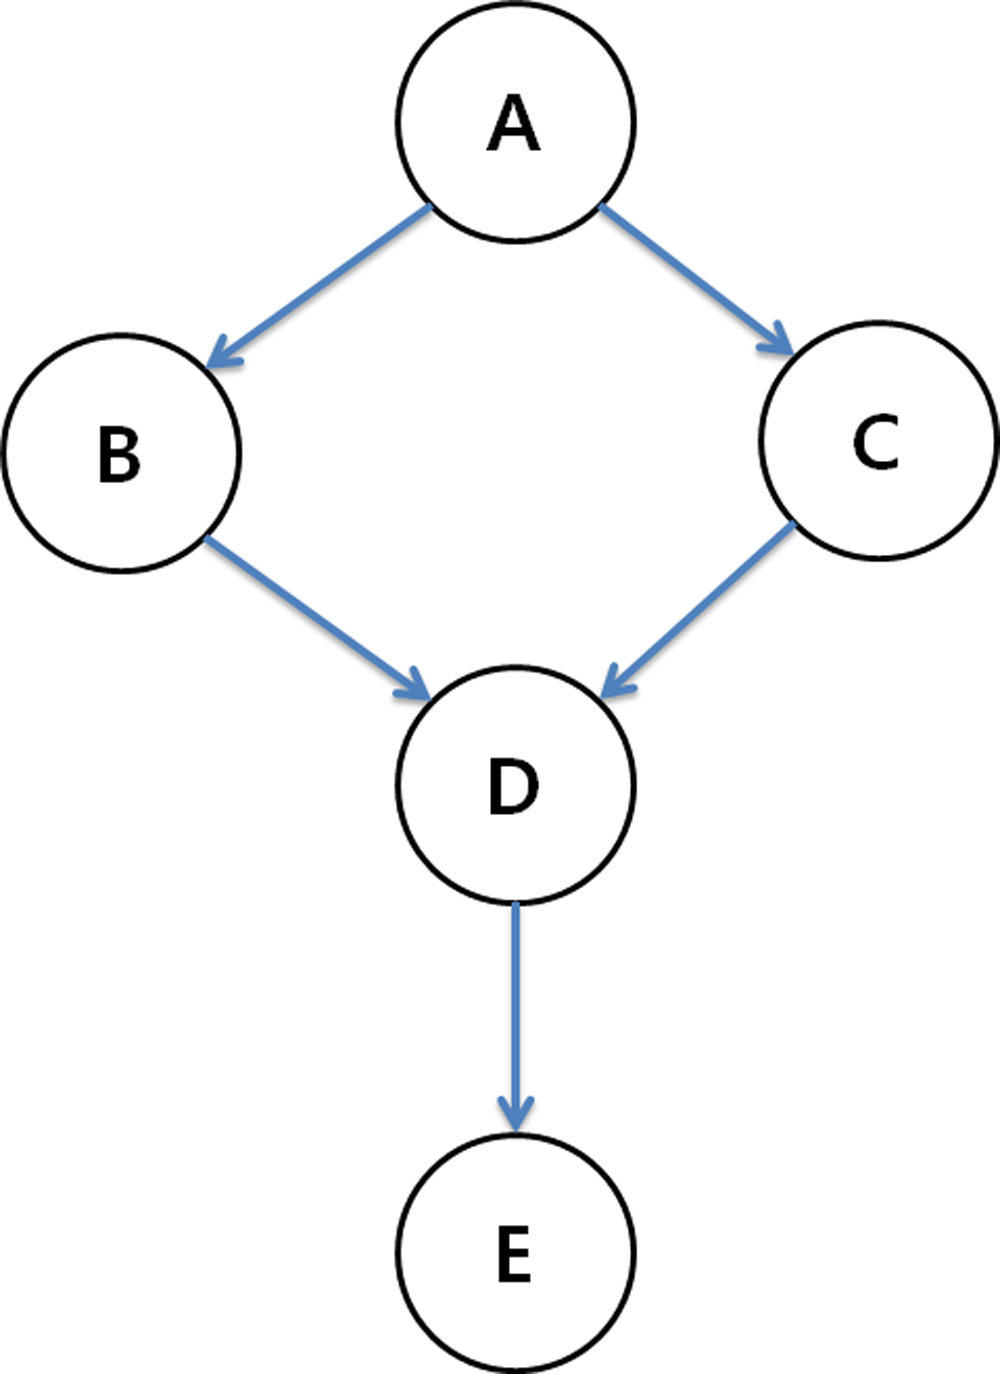
\includegraphics[height=150pt]{image01}
		\caption{$P(A,B,C,D,E)=P(A)P(B|A)P(C|A)P(D|B,C)P(E|D)$}
\end{figure}	

A BN defines a unique joint probability distribution over $X$ given by
$$P_{B}(X_{1},\cdots,X_{n})=\prod_{i=1}^{n}P_{B}(X_{i}|\prod_{X_{i}}).$$

\begin{itemize}
	\item A BN encodes the independence assumptions over the component random variables of $X$.
	
	\item An edge $(j, i)$ in $E$ represents a direct dependency of $X_{i}$ from $X_{j}$.
	
	\item The set of all Bayesian networks with $n$ variables is denotes by $B_{n}$.
\end{itemize}


\section{Bayesian Network Structure Learning}
~~~~The problem of learning a BN given data $T$ consists of finding the BN that best fits the data $T$. In order to quantify the fitting of a BN a scoring function $\phi$ is considered.

Learning a Bayesian network is as follows:

Given a data $T = \{y_{1}, \cdots, y_{n}\}$ and a scoring function $\phi$, the problem of learning a Bayesian network is to find a Bayesian network $B \in B_{n}$ that maximizes the value $\phi(B, T)$.

Bayesian network structure learning algorithms can be grouped into two categories by Marco Scutari (2010).

\begin{description}

	\item[Constraint-based algorithms] These algorithms learn the network structure by analyzing the probabilistic relations entailed by the Markov property of Bayesian networks with conditional independence tests and then constructing a graph which satisfies the corresponding d-separation statements. The resulting models are often interpreted as causal models even when learned from observational data (Pearl J. 1988).
	
	\item[Score-based algorithms] The main idea behind score-based learning is to optimize the degree of match between the generated network and the observations. (Benjamin B. Perry, 2003) These algorithms assign a score to each candidate Bayesian network and try to maximize it with some heuristic search algorithm. The search problem of identifying a Bayesian network that has a relative posterior probability greater than a given constant is NP-complete. (D.M. Chickering (1996)) Greedy search algorithms (such as hill-climbing or TABU search) are a common choice, but almost any kind of search procedure can be used.
\end{description}

Traditionally, in searching for a Bayesian network structure, the set of states was the set of all possible Bayesian network structures, the representation was a Directed Acyclic Graph(DAG) and the set of operators were various small local changes to a DAG, e.g. adding, removing or reversing an arc, as illustrated in Figure 1.2. (Ronan D. and Qiang S. 2007)

\begin{figure}[!h]
	\centering
		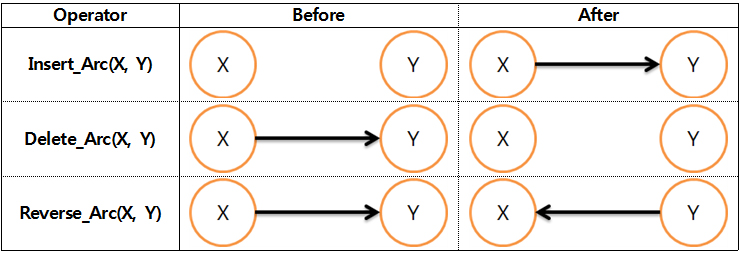
\includegraphics[height=100pt]{DAG_Operators}
		\caption{Basic Modification Operators in Searching for a Bayesian Network Structure}
\end{figure}	






\chapter{Bayesian Network Structure Learning Algorithms in bnlearn Package}
~~~~\textbf{bnlearn} is an R package which includes several algorithms for learning the structure of Bayesian networks with either discrete or continuous variables. Both constraint-based and score-based algorithms are implemented. (Marco S., 2010)

%
\section{Constraint-based Algorithms}
\subsection{Grow-Shrink (GS) Markov Blanket Algorithm}
~~~~Based on the Grow-Shrink Markov Blanket, the simplest Markov blanket detection algorithm (Margaritis, 2003) used in a structure learning algorithm.

The definition of a Markov blanket is as follows: for any variable $X \in U$, the Markov blanket $BL(X) \subseteq U$ is any set of variables such that for any $Y \in U - BL(X) - \{X\}, X \perp Y | BL(X)$. In other words, $BL(X)$ completely "shields" (d-separates) variable $X$ from any other variable outside $BL(X) \cup \{X\}$.

In a Bayesian network graph, the Markov blanket of a node includes its parents, children and other parents of all of its children.

\begin{center}\rule[0.5ex]{0.9\columnwidth}{1pt}\end{center}

\textbf{Algorithm.} \underline{The GS Markov Blanket Algorithm}

\begin{enumerate}
	\item $S \leftarrow NULL$
	
	\item \textbf{While} $\exists$ $Y\in U-\{X\}$
	
	~~~~such that $Y \not\perp X | S$,
	
	~~~~\textbf{do} $S \leftarrow S \cup \{Y\}$. (Growing phase)
	
	~~~~\textbf{End While}
	
	\item \textbf{While} $\exists$ $Y\in S$
	
	~~~~such that $Y \perp X | S - \{Y\}$,
	
	~~~~\textbf{do} $S \leftarrow S - \{Y\}$. (Shrinking phase)
	
	~~~~\textbf{End While}
	
	\item $B(X) \leftarrow S$.
\end{enumerate}

\begin{center}\rule[0.5ex]{0.9\columnwidth}{1pt}\end{center}

GS, for the recovery of the Markov blanket of $X$ is based on pairwise independent tests. It consists of two phases, a growing and a shrinking one. Starting from an empty set $S$, the growing phase adds variables to $S$ as long as they are dependent with $X$ given the current contents of $S$.

\subsection{Incremental Association (IAMB) Algorithm}
~~~~Based on the Incremental Association Markov blanket (IAMB) algorithm (Tsamardinos I. \emph{et al.} 2003), which is based on a two-phase selection scheme (a forward selection followed by an attempt to remove false positives).

\begin{center}\rule[0.5ex]{0.9\columnwidth}{1pt}\end{center}

\textbf{Algorithm.} \underline{The IAMB Algorithm}

\begin{enumerate}
	\item (Forward phase)
	
	~~~~$S \leftarrow NULL$
	
	~~~~\textbf{While} $S$ has changed
	
	~~~~~~~~\textbf{Find} the feature $X$ in $V-S-\{T\}$ that maximizes $f(X ; T|S)$
	
	~~~~~~~~\textbf{If} not $I(X ; T|S)$
	
	~~~~~~~~~~~~\textbf{Add} $X$ to $S$
	
	~~~~~~~~\textbf{End If}
	
	~~~~\textbf{End While}
	
	\item (Backward phase)

	~~~~\textbf{Remove} from $S$ all variables $X$, for which $I(X ; T|S-\{X\})$
	
	\item \textbf{Return} $S$
\end{enumerate}

\begin{center}\rule[0.5ex]{0.9\columnwidth}{1pt}\end{center}

IAMB consists of two phases, a forward and a backward one.

The Markov blanket of a variable of interest $T$, will be denotes as $MB(T)$. An estimate of the $MB(T)$ is kept in the set $S$. In the forward phase all variables that belong in $MB(T)$ and possibly more (false positives) enter $S$ while in the backward phase the false positives are identified and removed so that $S = MB(T)$ in the end.

The heuristic used in IAMB to identify potential Markov blanket members in 'forward phase' is the following:

Start with an empty candidate set for the $S$ and admit into it (in the next iteration) the variable that maximizes a heuristic function $f(X ; T|S)$. Function $f$ should return a non-zero value for every variable that is a member of the Markov blanket for the algorithm to be sound, and is typically a measure of association between $X$ and $T$ given $S$. In our experiments we used $f$ as the Mutual Information similar to what was suggested in Margaritis D. and Thrun S. (1999), J. Cheng \emph{et al.} (2002): $f(X; T|S)$ is the Mutual Information between $S$ and $T$ given $S$. It is important that $f$ is an informative and effective heuristic so that the set of candidate variables after 'forward phase' is as small as possible for two reasons: one is time efficiency (i.e. do not spend time considering irrelevant variables) and another is sample efficiency (do not require sample larger than what is absolutely necessary to perform conditional tests of independence).

In backward conditioning we remove features that do not belong to the $MB(T)$ one-by-one by testing whether a feature $X$ from $S$ is independent of $T$ given the remaining $S$.	

%
\section{Score-Based Algorithms}	
\subsection{Hill-Climbing (HC) Algorithm}
~~~~A Hill-climbing is a greedy search on the space of the directed graphs. The optimized implementation uses score caching, score decomposability and score equivalence to reduce the number of duplicated tests.

\begin{center}\rule[0.5ex]{0.9\columnwidth}{1pt}\end{center}

\textbf{Algorithm.} \underline{The Hill-climbing(HC) Algorithm}

\begin{enumerate}
	\item \textbf{Current}: Make$\_$Node(Initial State)
	
	\item \textbf{While}
	
	~~~~\textbf{Neighbor}: a highest-valued successor of Current.State
	
	~~~~\textbf{If} Neighbor.Value $<$ Current.Value \textbf{Then}
	
	~~~~~~~~\textbf{Return} Current.State
	
	~~~~\textbf{End If}
	
	~~~~Current $\leftarrow$ Neighbor
	
	\textbf{End While}
\end{enumerate}

\begin{center}\rule[0.5ex]{0.9\columnwidth}{1pt}\end{center}

It is simply a loop that continually moves in the direction of increasing value. The algorithm does not maintain a search tree, so the data structure for the current node only needs to record the state and the value of the objective function. Hill-climbing does not look beyond the immediate neighbors of the current state. This resembles trying to find the top of Mount Everest in a thick fog while suffering from amnesia. (Russell S. J. and Norvig P., 2009)

\subsection{TABU Search Algorithm}
~~~~A modified Hill-climbing is able to escape local optima by selecting a network that minimally decreases the score function.

A variant of Hill-climbing called TABU search has gained popularity (Fred W. G. and Manuel L., 1997). This algorithm maintains a TABU list of $k$ previously visited states that cannot be revisited, as well as improving efficiency when searching graphs. This list allows the algorithm to escape from some local minima.

\begin{center}\rule[0.5ex]{0.9\columnwidth}{1pt}\end{center}

\textbf{Algorithm.} \underline{The TABU Search Algorithm}

\begin{enumerate}
	\item Choose $x \in X$ to start the precess.
	
	\item Find $x' \in N(x)$ such that $f(x') < f(x)$.
	
	\item If no such $x'$ can be found, $x$ is the local optimum and the method stops.
	
	\item Otherwise, designate $x'$ to be the new $x$ and go to 2.
\end{enumerate}

\begin{center}\rule[0.5ex]{0.9\columnwidth}{1pt}\end{center}

TABU search begins in the same way as ordinary local or neighborhood search, proceeding iteratively from one point solution to another until a chosen termination criterion is satisfied. Each $x \in X$ has an associated neighborhood $N(x) \subset X$, and each solution $x' \in N(x)$ is reached from x by an operation called 'move'.

As an initial point of departure, we may contrast TABU search with a simple descent method where the goal is to $\min f(x)$ (or a corresponding ascent method where the goal is to $\max f(x)$). Such method only permits moves to neighbor solutions that improve the current objective function value and ends when no improving solutions can be found. A pseudo-code of a generic descent method is presented in 'Algorithm'. The final $x$ obtained by a descent method is called a local optimum, since it is at least as good or better than all solutions in its neighborhood. The evident shortcoming of a descent method is that such a local optimum in most cases will not be a global optimum, i.e., it usually will not minimize $f(x)$ over all $x \in X$.

%
\section{Hybrid Algorithms}
\subsection{Max-Min Hill-Climbing (MMHC) Algorithm}
~~~~A hybrid algorithm which combines the Max-Min Parents and Children algorithm (to restrict the search space) and the Hill-Climbing algorithm (to find the optimal network structure in the restricted space). (Tsamardinos I. \emph{et al.}, 2006)

The algorithm first identifies the parents and children set of each variable, then performs a greedy hill-climbing search in the space of Bayesian networks. The search begins with an empty graph. The edge addition, deletion, or direction reversal that leads to the largest increase in score is taken and the search continues in a similar fashion recursively.

\subsection{More general 2-phase Restricted Maximization (RSMAX2)}
~~~~A more general method is which Max-Min Hill-Climbing, uses any combination of constraint-based and score-based algorithms.





\chapter{The Comparison Methodology}
\section{The Number of Graphical Errors in the Learnt Structure}
~~~~The comparison methodology used in this paper is similar to the method used in X.-w. Chen \emph{et al.} (2006). The existence of the known network structures allows us to define three important terms which indicate the performance of the algorithm (in terms of the number of graphical errors in the learnt structure).

\begin{description}
	\item[C (Correct Arcs)] Edges present in the original network and in the learnt network structure.

	\item[M (Missing Arcs)] Edges present in the original network but not in the learnt network structure.
	
	\item[WO (Wrongly Oriented Arcs)] Edges present in the learnt network structure, but having opposite orientation when compared with the corresponding edge in the original network structure.
	
	\item[WC (Wrongly Corrected Arcs)] Edges not present in the original network but included in the learnt network structure.
\end{description}

\section{Network Scores}
~~~~The values of the BDe, the Log-likelihood (LL), the AIC, and the BIC are metrics for the learned networks. (Alexandra M. C., 2009) These measures can offer an idea of the quality of the networks from different points of view. In all four cases, the higher the value of the metric, the better the network. (D. Heckerman \emph{et al.}, 1995, Silvia A. \emph{et al.}, 2004).

\subsection{Bayesian Scoring Functions}
~~~~Compute the posterior probability distribution, starting from a prior probability distribution on the possilbe networks, conditioned to data $T$, that is, $P(B|T)$.

The best network is the one that maximizes the posterior probability.

Since the term $P(T)$ is the same for all possible networks, in practice, for comparative purposes, computing $P(B, T)$ is sufficient.

As it is easier to work in the logarithmic space, the scoring functions use the value $\log(P(B,T))$ instead of $P(B,T)$.

\subsubsection{BDe}
~~~~D. Heckerman \emph{et al.} (1995) proposed the Bayesian Dirichlet (BDe) score.

Given a directed acyclic graph (DAG) $G$ such that $P(G)>0$ then $\varTheta_{ij}$ is Dirichlet for all $\varTheta_{ij}$ in $\varTheta_{G}$. And given a Bayesian network $B$, data $T$ can be seen as a multinomial sample of the joint space $D$ with parameters
$$\Theta_{D}=\{\theta_{x_{1},\cdots,x_{n}}\}_{x_{i}=1,\cdots,r_{i},i\in1,\cdots,n}$$

where $\theta_{x_{1}, \cdots, x_{n}} = \prod_{i=1}^{n}\theta_{x_{I}|\prod_{x_{i}}}$.

For any complete $G$, we have that $P(G) > 0$. Then $\rho(\varTheta_{G}|G)=\prod_{i=1}^{n}\rho(\varTheta_{i}|G)$ (global parameter independence) and $\rho(\varTheta_{i}|G)=\prod_{i=1}^{q_{i}}\rho(\varTheta_{ij}|G)$ for all $i=1,\cdots,n$ (local parameter independence).

Given two DAGs $G$ and $G'$, such that $P(G)>0$ and $P(G')>0$, if $X_{i}$ has the same parents in $G$ and $G_{0}$, then $\rho(\varTheta_{ij}|G)=\rho(\varTheta_{ij}|G')$ for all $j=1,\cdots,q_{i}$.

Suppose that $\rho(\Theta_{D}|G)$ is Dirichlet with equivalent sample size $N'$ for some complete $G$ in $D$. Then, for any Bayesian network $B$ in $D$,
$$BDe(B,T) = P(B,T)=P(B)\times\prod_{i=1}^{n}\prod_{j=1}^{q_{i}}(\frac{\Gamma(N'_{ij})}{\Gamma(N_{ij}+N'_{ij})}\times\prod_{k=1}^{r_{i}}\frac{\Gamma(N_{ijk}+N'_{ijk})}{\Gamma(N'_{ijk})})$$

where $N'_{ijk} = N' \times P(X_{i} = x_{ik}, \prod_{X_{i}} = \omega_{ij}|G)$.

The equivalent sample size $N'$ expresses the strength of out belief in the prior distribution.

\subsection{Information-theoretic Scoring Functions}
\subsubsection{$\log$-likelihood (LL)}
~~~~The \textbf{$\log$-likelihood (LL) Score} is defined in the following way:
$$LL(B|T)=\sum_{i=1}^{n}\sum_{j=1}^{q_{i}}\sum_{k=1}^{r_{i}}N_{ijk}\log(\frac{N_{ijk}}{N_{ij}}).$$

The LL score tends to favor complete network structures and it does not provide an useful representation of the independence assumptions of the learned network.

This phenomenon of overfitting is usually avoided in two different ways:

\begin{itemize}
	\item By limiting the number of parents per network variable.
	
	\item By using some penalization factor over the LL score : AIC, BIC
\end{itemize}

\subsubsection{AIC and BIC}
The measure of the quality of a BN can be computed in several different ways:

$$\phi(B|T) = LL(B|T) - f(N)|B|,$$

where $f(N)$ is a non-negative penalization function.

\begin{itemize}
	\item If f(N) = 1, we have the \textbf{Akaike Information Criterion (AIC)} scoring function:
	
	$$AIC(B|T) = LL(B|T) - |B|.$$
	
	\item If $f(N) = \frac{1}{2} \log(N)$, we have the \textbf{Bayesian Information Criterion (BIC)} score.
	
	\item If $f(N) = 0$, we have the LL score.
\end{itemize}





\chapter{Data Generation with BN$\_$Data$\_$Generator in R}
~~~~If given a Bayesian network models, then we can make data set based on model. However, it does not provide by \textbf{bnlearn}, in addition, it was difficult to find other functions. It makes very hard work to create data in \textbf{R}. Other tools suffer from serious trade off between cost and complexity, restricting most studies relevant to Bayesian network to using only real data.

To address such problem, a data generator based on Bayesian network model using R is built and introduced. At present, exists as R functional form, and it is planning to make an R package. It  published an update on the current status at https://github.com/praster1/BN$\_$Data$\_$Generator. This generator was declared the GNU 2.0 license.

\section{BN$\_$Data$\_$Generator Function in R}
\begin{description}
	\item[Description] It based on a Bayesian network model to generates synthetic data.
	
	\item[Usage] BN$\_$Data$\_$Generator (arcs, input$\_$Probs, n, node$\_$names)
	
	\item[Arguments]
\end{description}
	
\begin{table}[!h]
\centering	\caption{Argunemts of BN$\_$Data$\_$Generator}
{\tabcolsep=0.01in																										
	\begin{tabular}{c|c|l}
	\hline
	Argument & Type & ~~Description\tabularnewline
	\hline
	arcs & matrix & ~~A matrix that determines the arcs\tabularnewline
	input\_Probs & list & ~~The conditional probabilities.\tabularnewline
	n & constant & ~~sample size\tabularnewline
	node\_names & vector & ~~node names\tabularnewline
	\hline
	\end{tabular}
}																										
\end{table}

\section{A Simple Example}
~~~~Suppose we generate a data based on the model as show in Figure 4.1. This model is the "Bayesian network model of Asia Data Set by Lauritzen and Spiegelhalter" to be introduced in the next chapter.

\begin{figure}[t]
	\centering
	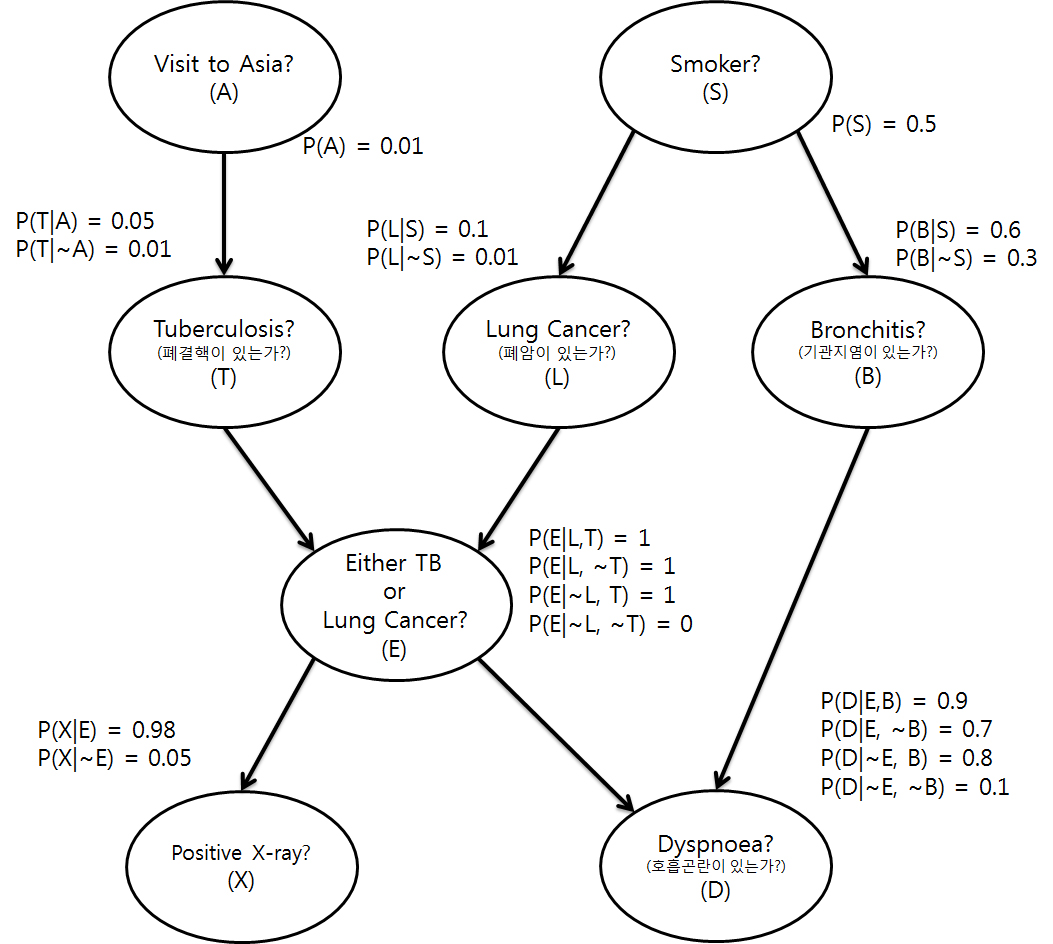
\includegraphics[height=250pt]{images/Real_Asia}
	\caption{BN model of Asia Data Set by Lauritzen and Spiegelhalter}
\end{figure}

It makes Arcs, input$\_$Probs, node$\_$names as follows:

\begin{center}\rule[0.5ex]{0.9\columnwidth}{1pt}\end{center}

R$>$ arcs = rbind(

		~~~~~~~~$\#$	A	S	T	L	B	E	X	D
		
		~~~~~~~~c(0,	0,	1,	0,	0,	0,	0,	0),	$\#$A
		
		~~~~~~~~c(0,	0,	0,	1,	1,	0,	0,	0),	$\#$S
		
		~~~~~~~~c(0,	0,	0,	0,	0,	1,	0,	0),	$\#$T
		
		~~~~~~~~c(0,	0,	0,	0,	0,	1,	0,	0),	$\#$L
		
		~~~~~~~~c(0,	0,	0,	0,	0,	0,	0,	1),	$\#$B
		
		~~~~~~~~c(0,	0,	0,	0,	0,	0,	1,	1),	$\#$E
		
		~~~~~~~~c(0,	0,	0,	0,	0,	0,	0,	0),	$\#$X
		
		~~~~~~~~c(0,	0,	0,	0,	0,	0,	0,	0))	$\#$D
		
R$>$ arc$\_$name = c("A", "S", "T", "L", "B", "E", "X", "D")

R$>$ Probs = list(

	~c(0.01),						$\# P(A)$
	
	~c(0.5), 						$\# P(S)$
	
	~c(0.05, 0.01),				$\# P(T|A), P(T|\sim A)$
	
	~c(0.1, 0.01),				$\# P(L|S), P(L|\sim S)$
	
	~c(0.6, 0.3),					$\# P(B|S), P(B|\sim S)$
	
	~c(1, 1, 1, 0),				$\# P(E|T,L), P(E|\sim T,L), P(E|T,\sim L), P(E|\sim T,\sim L)$
	
	~c(0.98, 0.05),				$\# P(X|E), P(X|\sim E)$

	~$\# P(D|B,E), P(D|\sim B,E), P(D|B,\sim E), P(D|\sim B,\sim E)$
	
	~c(0.9, 0.7, 0.8, 0.1))

\begin{center}\rule[0.5ex]{0.9\columnwidth}{1pt}\end{center}

Suppose the sample size is 1000. If you type objects and sample size into BN$\_$Data$\_$Generator, then the data is generated.

\begin{center}\rule[0.5ex]{0.9\columnwidth}{1pt}\end{center}

R$>$ n = 1000
 
R$>$ res = BN$\_$Data$\_$Generator(arcs, Probs, n, arc$\_$name)

R$>$ data = res$\$$data

R$>$ head(data)

~~~~~~A S T L B E X D
  
~~~~1 N N N N N N N N

~~~~2 N Y N N Y N N Y

~~~~3 N N N N N N N N

~~~~4 N Y N N N N N N

~~~~5 N N N N Y N N N

~~~~6 N Y N N Y N N Y

R$>$ dim(data)

~~~~[1] 1000    8

\begin{center}\rule[0.5ex]{0.9\columnwidth}{1pt}\end{center}

\begin{figure}[h]
	\centering
	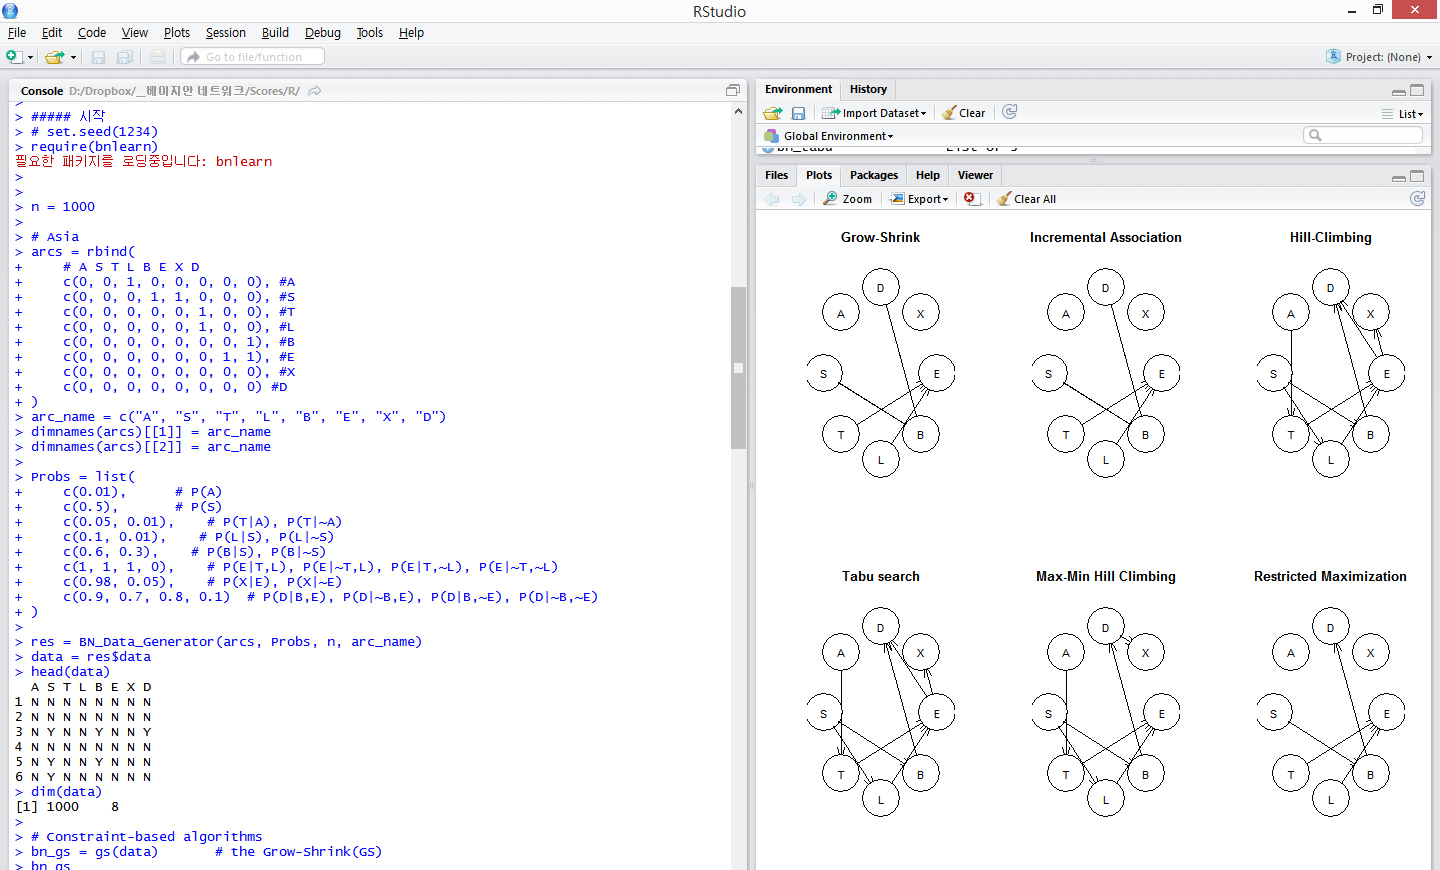
\includegraphics[height=250pt]{images/image23}
	\caption{After make a data, execution results by bnlearn}
\end{figure}





\chapter{Simulation}
~~~~Previous tools suffer from a serious trade-off between cost and complexity, restricting most studies relevant to Bayesian network to using only real data.

Therefore, in this paper, have been widely used so far, for the BN demonstration model, I tried to first apply the algorithm.

However, in order to measure the objective performance of the algorithm, it is necessary to try to analyze the synthetic data. Therefore, in this paper, by using the data generator BN that introduced, after generating the synthetic data in accordance with the topology, and algorithms were attempted to be applied to this.

In order to avoid the influence of chance, all experiments are repeated 100 times, and overall results are reported.

% Real Data
\section{Real Data}
\subsection{Asia Data Set by Lauritzen and Spiegelhalter}
\begin{description}
	\item[Description] Small synthetic data set from Lauritzen S. and Spiegelhalter D. (1988) about lung diseases (tuberculosis, lung cancer or bronchitis) and visits to Asia.

	\item[Number of nodes] 8
	
	\item[Number of arcs] 8
	
	\item[Number of parameters] 18
\end{description}

Lauritzen S. and Spiegelhalter D. (1988) motivate this example as follows:

"Shortness-of-breath (dyspnoea) may be due to tuberculosis, lung cancer or bronchitis, or none of them, or more than one of them. A recent visit to Asia increases the chances of tuberculosis, while smoking is known to be a risk factor for both lung cancer and bronchitis. The results of a single chest X-ray do not discriminate between lung cancer and tuberculosis, as neither does the presence or absence of dyspnoea."

\begin{table}[p]
\centering	\caption{Comparison of scores and correct arcs via Asia data set} \tiny	
{\tabcolsep=0.01in
	\begin{tabular}{cc||cc|cc|cc||cc|cc|cc|cc}
		\hline	
		& & \multicolumn{14}{c}{Asia (Num of Nodes = 8)}\tabularnewline	
		\hline	
		\multicolumn{2}{c||}{Sample Size} & \multicolumn{2}{c|}{1000} & \multicolumn{2}{c|}{5000} & \multicolumn{2}{c||}{10000} & & & \multicolumn{2}{c|}{1000} & \multicolumn{2}{c|}{5000} & \multicolumn{2}{c}{10000}\tabularnewline	
		\hline	
		& & Sum. & Std.Dev. & Sum. & Std.Dev. & Sum. & Std.Dev. & & & Sum. & Std.Dev. & Sum. & Std.Dev. & Sum. & Std.Dev.\tabularnewline
		\hline	
		\hline	
		\multirow{4}{*}{BDe} & HC & -229814 & 35.25 & -1113883 & 85.65 & -2218508 & 126.41 & \multirow{4}{*}{C} & HC & 677 & 0.55 & 716 & 0.37 & 735 & 0.48\tabularnewline	
		& TABU & -229806 & 35.29 & -1113857 & 85.9 & -2218431 & 126.4 & & TABU & 655 & 0.73 & 677 & 0.72 & 703 & 0.76\tabularnewline	
		& MMHC & -249829 & 41.68 & -1213021 & 117.02 & -2417769 & 191.84 & & MMHC & 461 & 0.55 & 503 & 0.48 & 514 & 0.59\tabularnewline	
		& RSMAX2 & -252800 & 43.81 & -1233095 & 121.09 & -2457976 & 173.35 & & RSMAX2 & 400 & 0 & 400 & 0 & 400 & 0\tabularnewline	
		\hline	
		\multirow{4}{*}{loglik} & HC & -220520 & 36.46 & -1102564 & 85.92 & -2206160 & 126.05 & \multirow{4}{*}{M} & HC & 122 & 0.52 & 83 & 0.38 & 65 & 0.48\tabularnewline	
		& TABU & -220505 & 36.54 & -1102521 & 86.31 & -2206030 & 126.02 & & TABU & 122 & 0.52 & 83 & 0.38 & 65 & 0.48\tabularnewline	
		& MMHC & -241431 & 43.03 & -1202710 & 117.97 & -2406616 & 192.19 & & MMHC & 339 & 0.55 & 297 & 0.48 & 286 & 0.59\tabularnewline	
		& RSMAX2 & -244901 & 44.97 & -1223631 & 121.63 & -2447783 & 173.8 & & RSMAX2 & 400 & 0 & 400 & 0 & 400 & 0\tabularnewline	
		\hline	
		\multirow{4}{*}{AIC} & HC & -222238 & 36.46 & -1104349 & 85.87 & -2208092 & 126.21 & \multirow{4}{*}{WO} & HC & 1 & 0.1 & 1 & 0.1 & 0 & 0\tabularnewline	
		& TABU & -222226 & 36.53 & -1104315 & 86.16 & -2207985 & 126.19 & & TABU & 23 & 0.51 & 40 & 0.62 & 32 & 0.66\tabularnewline	
		& MMHC & -242973 & 43 & -1204336 & 117.81 & -2408295 & 192.1 & & MMHC & 0 & 0 & 0 & 0 & 0 & 0\tabularnewline	
		& RSMAX2 & -246201 & 44.97 & -1224936 & 121.62 & -2449114 & 173.8 & & RSMAX2 & 0 & 0 & 0 & 0 & 0 & 0\tabularnewline	
		\hline	
		\multirow{4}{*}{BIC} & HC & -226454 & 36.49 & -1110166 & 85.76 & -2215057 & 126.96 & \multirow{4}{*}{WC} & HC & 72 & 1.22 & 96 & 1.12 & 224 & 1.69\tabularnewline	
		& TABU & -226449 & 36.52 & -1110161 & 85.76 & -2215033 & 126.99 & & TABU & 112 & 1.43 & 170 & 1.46 & 292 & 2.02\tabularnewline	
		& MMHC & -246757 & 42.97 & -1209634 & 117.34 & -2414348 & 191.83 & & MMHC & 202 & 0.2 & 218 & 0.58 & 244 & 0.83\tabularnewline	
		& RSMAX2 & -249391 & 44.97 & -1229189 & 121.6 & -2453913 & 173.82 & & RSMAX2 & 0 & 0 & 8 & 0.39 & 50 & 0.87\tabularnewline	
		\hline	
	\end{tabular}
}
\end{table} 

	\begin{figure}[p]
	\centering
		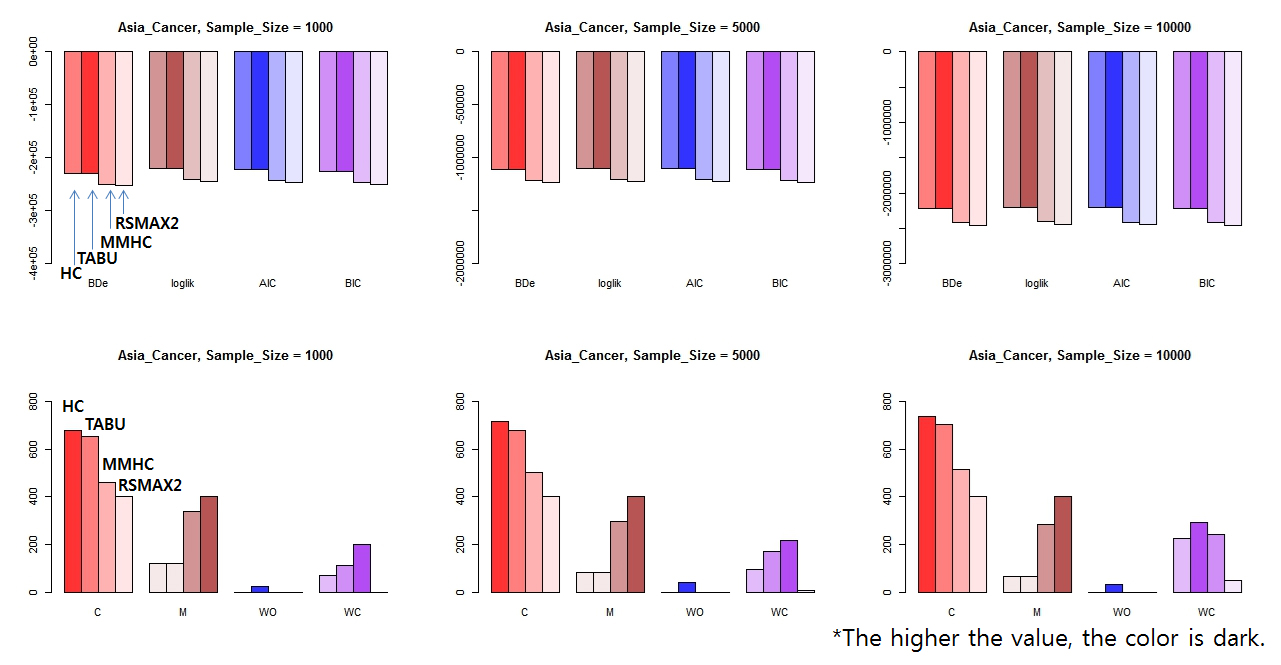
\includegraphics[height=220pt]{Real_1_Asia}
		\caption{Comparison of scores and correct arcs via Asia data set}
	\end{figure}	

\newpage{}

\subsection{Insurance Evaluation Network Data Set}
	\begin{figure}[h]
	\centering
		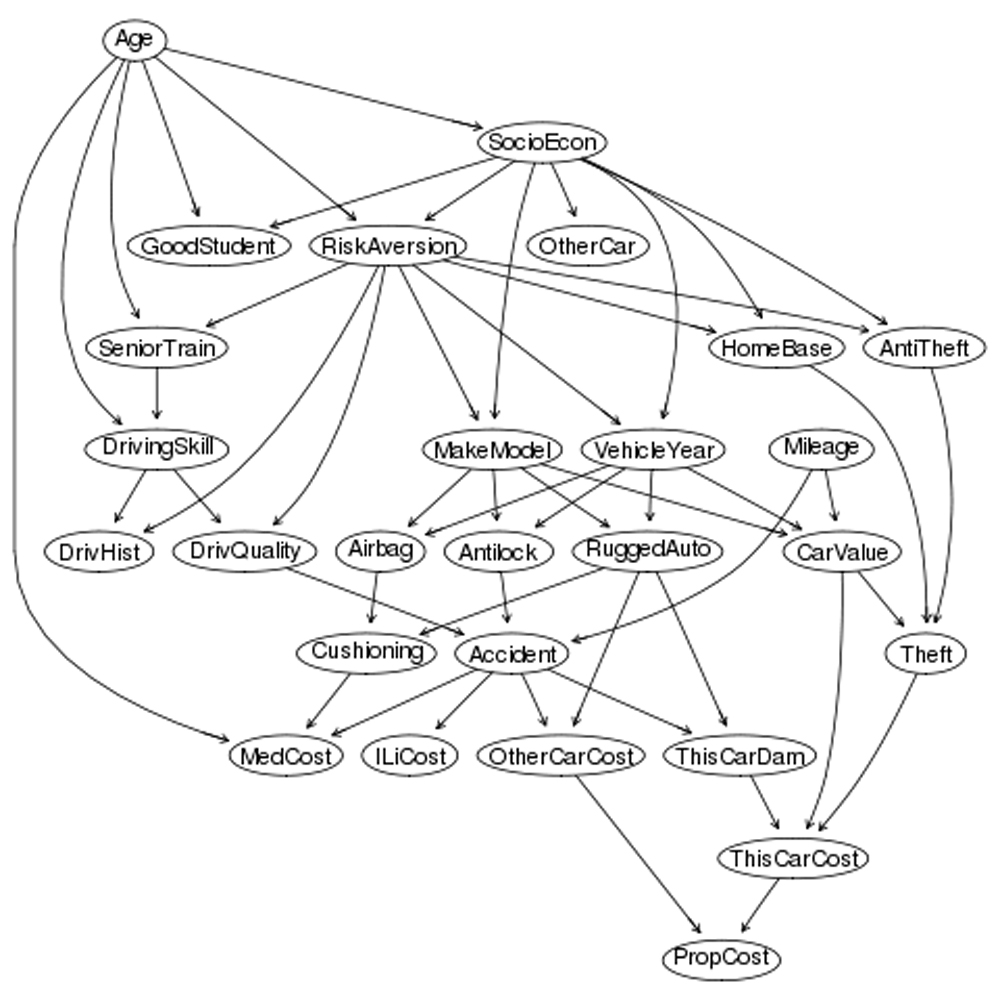
\includegraphics[height=200pt]{Real_Insurance}
		\caption{Bayesian network model of Insurance Evaluation Network Data Set}
	\end{figure}	

\begin{description}
	\item[Description] Insurance is a network for evaluating car insurance risks.

	\item[Number of nodes] 27
	
	\item[Number of arcs] 52
	
	\item[Number of parameters] 984
\end{description}

Binder J. \emph{et al.} (1997) motivate this example. This network for estimating the expected claim costs for a car insurance policyholder.

\begin{table}[p]																										
\centering	\caption{Comparison of scores and correct arcs via Insurance data set}	\tiny																						
{\tabcolsep=0.01in																										
\begin{tabular}{cc||cc|cc|cc||cc|cc|cc|cc}																										
\hline																										
&	&	\multicolumn{14}{c}{Insurance	(Num	of	Nodes	=	27)}\tabularnewline																			
\hline																										
\multicolumn{2}{c||}{Sample	Size}	&	\multicolumn{2}{c|}{1000}	&	\multicolumn{2}{c|}{5000}	&	\multicolumn{2}{c||}{10000}	&	&	&	\multicolumn{2}{c|}{1000}	&	\multicolumn{2}{c|}{5000}	&	\multicolumn{2}{c}{10000}\tabularnewline											
\hline																										
&	&	Sum.	&	Std.Dev.	&	Sum.	&	Std.Dev.	&	Sum.	&	Std.Dev.	&	&	&	Sum.	&	Std.Dev.	&	Sum.	&	Std.Dev.	&	Sum.	&	Std.Dev.\tabularnewline
\hline																										
\hline																										
\multirow{4}{*}{BDe} & HC &	-1427953 & 	113.01 & 	-6730331 & 	189.16 & 	-13298470 & 	246.4 & 	\multirow{4}{*}{C} & HC &	1864 & 	1.57 & 	2226 & 	0.85 & 	2414 & 	0.4\tabularnewline													
& TABU &	-1422716 & 	120.52 & 	-6708058 & 	190.97 & 	-13294810 & 	244.2 & 	& TABU &	1961 & 	1.98 & 	2543 & 	0.79 & 	2826 & 	0.68\tabularnewline													
& MMHC &	-1644392 & 	548.92 & 	-7281377 & 	826.67 & 	-14112976 & 	1680.81 & 	& MMHC &	1146 & 	1.82 & 	1457 & 	1.17 & 	1731 & 	1.88\tabularnewline													
& RSMAX2 &	-1735658 & 	397.81 & 	-8293044 & 	1714.16 & 	-16408869 & 	2342.35 & 	& RSMAX2 &	862 & 	1.42 & 	977 & 	1.77 & 	848 & 	0.61\tabularnewline													
\hline																										
\multirow{4}{*}{loglik} & HC &	-1347816 & 	118.57 & 	-6603841 & 	195.33 & 	-13134593 & 	257.01 & 	\multirow{4}{*}{M} & HC &	2253 & 	1.11 & 	1738 & 	0.79 & 	1413 & 	0.53\tabularnewline													
& TABU &	-1341071 & 	128.83 & 	-6580889 & 	194.64 & 	-13143085 & 	241.01 & 	& TABU &	2155 & 	1.39 & 	1642 & 	0.77 & 	1402 & 	0.43\tabularnewline													
& MMHC &	-1590326 & 	585.75 & 	-7192400 & 	852.4 & 	-14000007 & 	1736.44 & 	& MMHC &	3526 & 	2.2 & 	2849 & 	1.34 & 	2334 & 	2.5\tabularnewline													
& RSMAX2 &	-1687201 & 	417.78 & 	-8223919 & 	1734.08 & 	-16330085 & 	2362.44 & 	& RSMAX2 &	3761 & 	1.31 & 	3497 & 	1.05 & 	3469 & 	0.77\tabularnewline													
\hline																										
\multirow{4}{*}{AIC} & HC &	-1383888 & 	112.68 & 	-6652052 & 	190.99 & 	-13198494 & 	248.77 & 	\multirow{4}{*}{WO} & HC &	1083 & 	1.16 & 	1236 & 	0.73 & 	1373 & 	0.49\tabularnewline													
& TABU &	-1378131 & 	120.12 & 	-6629457 & 	191.37 & 	-13197529 & 	243.3 & 	& TABU &	1084 & 	1.56 & 	1015 & 	0.72 & 	972 & 	0.55\tabularnewline													
& MMHC &	-1607916 & 	566.08 & 	-7218618 & 	841.94 & 	-14033715 & 	1714.51 & 	& MMHC &	528 & 	1.39 & 	894 & 	0.76 & 	1135 & 	0.76\tabularnewline													
& RSMAX2 &	-1701145 & 	409.22 & 	-8241628 & 	1727.25 & 	-16350189 & 	2356.64 & 	& RSMAX2 &	577 & 	0.99 & 	726 & 	1.67 & 	883 & 	1.02\tabularnewline													
\hline																										
\multirow{4}{*}{BIC} & HC &	-1472404 & 	105.57 & 	-6809152 & 	185.18 & 	-13428868 & 	242.07 & 	\multirow{4}{*}{WC} & HC &	1810 & 	2.28 & 	2096 & 	1.49 & 	2240 & 	1.58\tabularnewline													
& TABU &	-1469072 & 	108.51 & 	-6787720 & 	191.17 & 	-13393809 & 	256.04 & 	& TABU &	1756 & 	2.49 & 	1906 & 	1.52 & 	1696 & 	1.46\tabularnewline													
& MMHC &	-1651080 & 	519.05 & 	-7304052 & 	808.56 & 	-14155238 & 	1635.76 & 	& MMHC &	1098 & 	2.35 & 	1494 & 	2.45 & 	1630 & 	1.43\tabularnewline													
& RSMAX2 &	-1735362 & 	389.69 & 	-8299334 & 	1705.3 & 	-16422667 & 	2335.81 & 	& RSMAX2 &	1120 & 	2.03 & 	1220 & 	1.69 & 	1596 & 	1.56\tabularnewline													
\hline																										
\end{tabular}																										
}																										
\end{table}

	\begin{figure}[p]
	\centering
		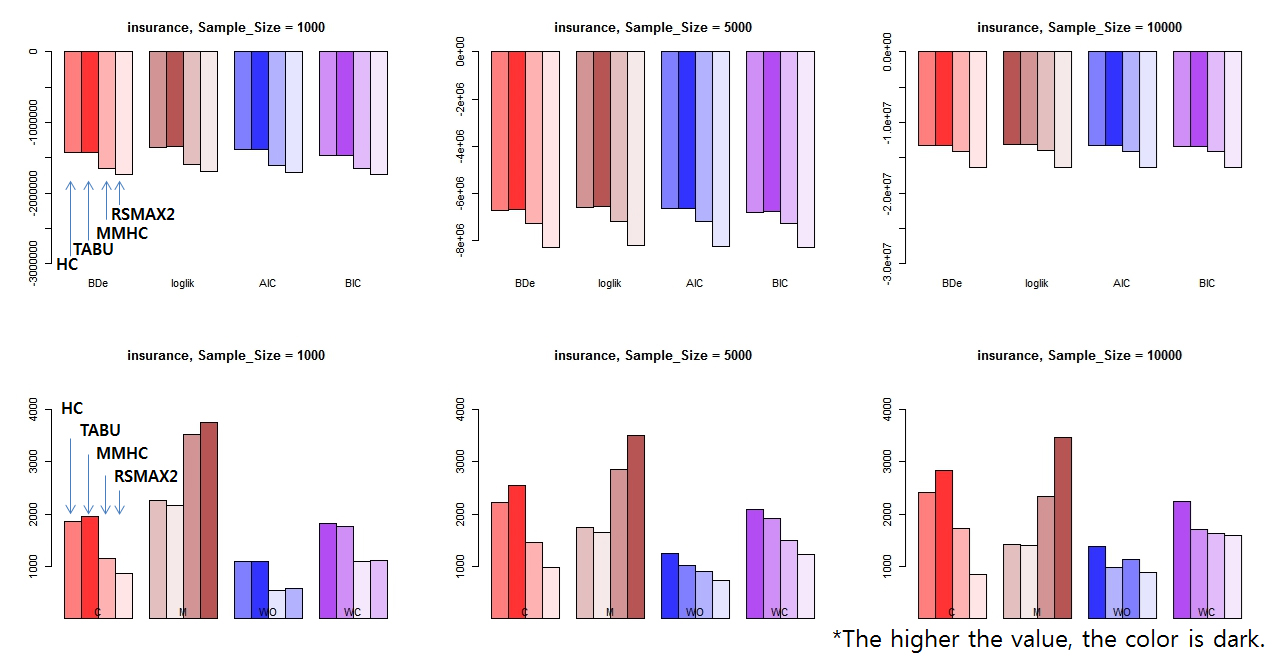
\includegraphics[height=220pt]{Real_2_Insurance}
		\caption{Comparison of scores and correct arcs via Insurance data set}
	\end{figure}	

\newpage{}

\subsection{ALARM Monitoring System Data Set}
	\begin{figure}[h]
	\centering
		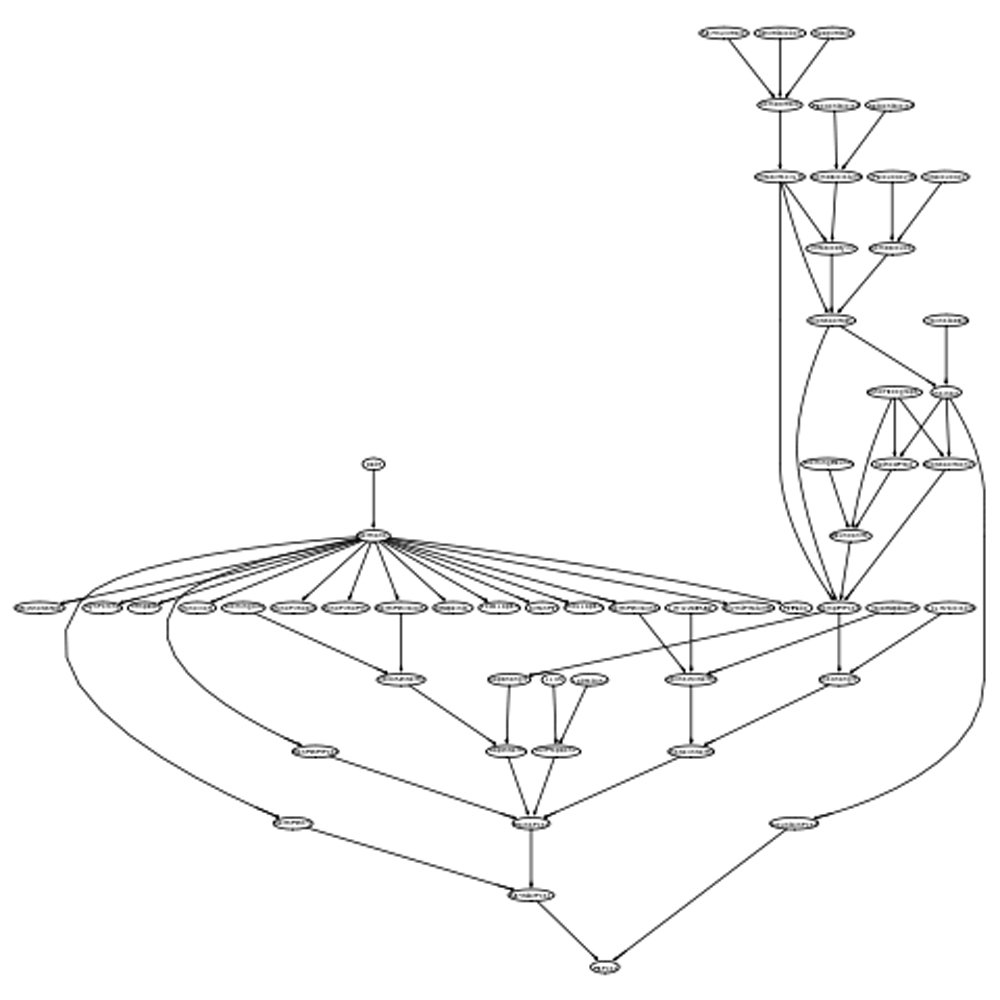
\includegraphics[height=200pt]{images/Real_Alarm}
		\caption{Bayesian network model of ALARM Monitoring System Data Set}
	\end{figure}	

\begin{description}
	\item[Description] The ALARM ("A Logical Alarm Reduction Mechanism") is a Bayesian network designed to provide an alarm message system for patient monitoring.

	\item[Number of nodes] 37
	
	\item[Number of arcs] 46
	
	\item[Number of parameters] 509
\end{description}

Beinlich I. \emph{et al.} (1989) motivate this example. ALARM (A Logical Alarm Reduction Mechanism) is a diagnostic application used to explore probabilistic reasoning techniques in belief networks. ALARM implements an alarm message system for patient monitoring: it calculates probabilities for a differential diagnosis based on available evidence.

% ALARM
\begin{table}[p]																										
\centering	\caption{Comparison of scores and correct arcs via ALARM data set}	\tiny																						
{\tabcolsep=0.01in																										
\begin{tabular}{cc||cc|cc|cc||cc|cc|cc|cc}																										
\hline																										
&	&	\multicolumn{14}{c}{ALARM	(Num	of	Nodes	=	37)}\tabularnewline																			
\hline																										
\multicolumn{2}{c||}{Sample	Size}	&	\multicolumn{2}{c|}{1000}	&	\multicolumn{2}{c|}{5000}	&	\multicolumn{2}{c||}{10000}	&	&	&	\multicolumn{2}{c|}{1000}	&	\multicolumn{2}{c|}{5000}	&	\multicolumn{2}{c}{10000}\tabularnewline											
\hline																										
&	&	Sum.	&	Std.Dev.	&	Sum.	&	Std.Dev.	&	Sum.	&	Std.Dev.	&	&	&	Sum.	&	Std.Dev.	&	Sum.	&	Std.Dev.	&	Sum.	&	Std.Dev.\tabularnewline
\hline																										
\hline																										
\multirow{4}{*}{BDe} & HC &	-1178527 & 	132.62 & 	-5580032 & 	259.61 & 	-11006608 & 	381.65 & 	\multirow{4}{*}{C} & HC &	2048 & 	1.73 & 	2283 & 	0.43 & 	2270 & 	0.96\tabularnewline													
& TABU &	-1177619 & 	133.2 & 	-5580099 & 	246.64 & 	-11005176 & 	380.57 & 	& TABU &	2426 & 	1.8 & 	2709 & 	1.05 & 	2686 & 	1.26\tabularnewline													
& MMHC &	-1673651 & 	649.54 & 	-7510018 & 	2077.76 & 	-13885378 & 	7417.41 & 	& MMHC &	1051 & 	1.77 & 	1421 & 	1.75 & 	1925 & 	3.09\tabularnewline													
& RSMAX2 &	-1735940 & 	439.39 & 	-8318508 & 	2058.09 & 	-16586602 & 	3307.55 & 	& RSMAX2 &	633 & 	1.65 & 	867 & 	0.92 & 	858 & 	1.19\tabularnewline													
\hline																										
\multirow{4}{*}{loglik} & HC &	-1099997 & 	130.61 & 	-5464607 & 	260.53 & 	-10860805 & 	370.7 & 	\multirow{4}{*}{M} & HC &	900 & 	1.06 & 	498 & 	0.4 & 	468 & 	0.69\tabularnewline													
& TABU &	-1099325 & 	130.77 & 	-5465405 & 	244.34 & 	-10861471 & 	371.47 & 	& TABU &	878 & 	0.97 & 	501 & 	0.36 & 	468 & 	0.69\tabularnewline													
& MMHC &	-1617451 & 	672.21 & 	-7426574 & 	2093.3 & 	-13790813 & 	7449.01 & 	& MMHC &	2460 & 	1.68 & 	1480 & 	1.04 & 	1268 & 	1.56\tabularnewline													
& RSMAX2 &	-1682617 & 	453.09 & 	-8242927 & 	2079.53 & 	-16508716 & 	3325.33 & 	& RSMAX2 &	3286 & 	1.6 & 	3162 & 	1.21 & 	2949 & 	1.05\tabularnewline													
\hline																										
\multirow{4}{*}{AIC} & HC &	-1135950 & 	129.48 & 	-5509035 & 	253.54 & 	-10923175 & 	374.81 & 	\multirow{4}{*}{WO} & HC &	1652 & 	1.37 & 	1819 & 	0.46 & 	1862 & 	0.9\tabularnewline													
& TABU &	-1134574 & 	130.77 & 	-5508543 & 	244.04 & 	-10921249 & 	372.87 & 	& TABU &	1296 & 	1.52 & 	1390 & 	0.96 & 	1446 & 	1.27\tabularnewline													
& MMHC &	-1634699 & 	655.42 & 	-7451159 & 	2085 & 	-13816106 & 	7435.45 & 	& MMHC &	1089 & 	1.38 & 	1699 & 	2.05 & 	1407 & 	1.98\tabularnewline													
& RSMAX2 &	-1698026 & 	443.88 & 	-8266708 & 	2064.51 & 	-16527481 & 	3318.41 & 	& RSMAX2 &	681 & 	1.6 & 	571 & 	0.98 & 	793 & 	0.71\tabularnewline													
\hline																										
\multirow{4}{*}{BIC} & HC &	-1224175 & 	130.11 & 	-5653808 & 	251.23 & 	-11148029 & 	416.51 & 	\multirow{4}{*}{WC} & HC &	2498 & 	2.58 & 	2306 & 	1.9 & 	2714 & 	1.56\tabularnewline													
& TABU &	-1221071 & 	133.9 & 	-5649112 & 	244.7 & 	-11136759 & 	427.99 & 	& TABU &	2314 & 	2.48 & 	2032 & 	2.08 & 	2452 & 	2.25\tabularnewline													
& MMHC &	-1677023 & 	614.97 & 	-7531272 & 	2058.32 & 	-13907292 & 	7386.76 & 	& MMHC &	1934 & 	2.22 & 	2890 & 	2.61 & 	2368 & 	2.84\tabularnewline													
& RSMAX2 &	-1735838 & 	423.78 & 	-8344201 & 	2018.29 & 	-16595132 & 	3293.99 & 	& RSMAX2 &	1684 & 	2.73 & 	1982 & 	2.56 & 	2262 & 	1.96\tabularnewline													
\hline																										
\end{tabular}																										
}																										
\end{table}

	\begin{figure}[p]
	\centering
		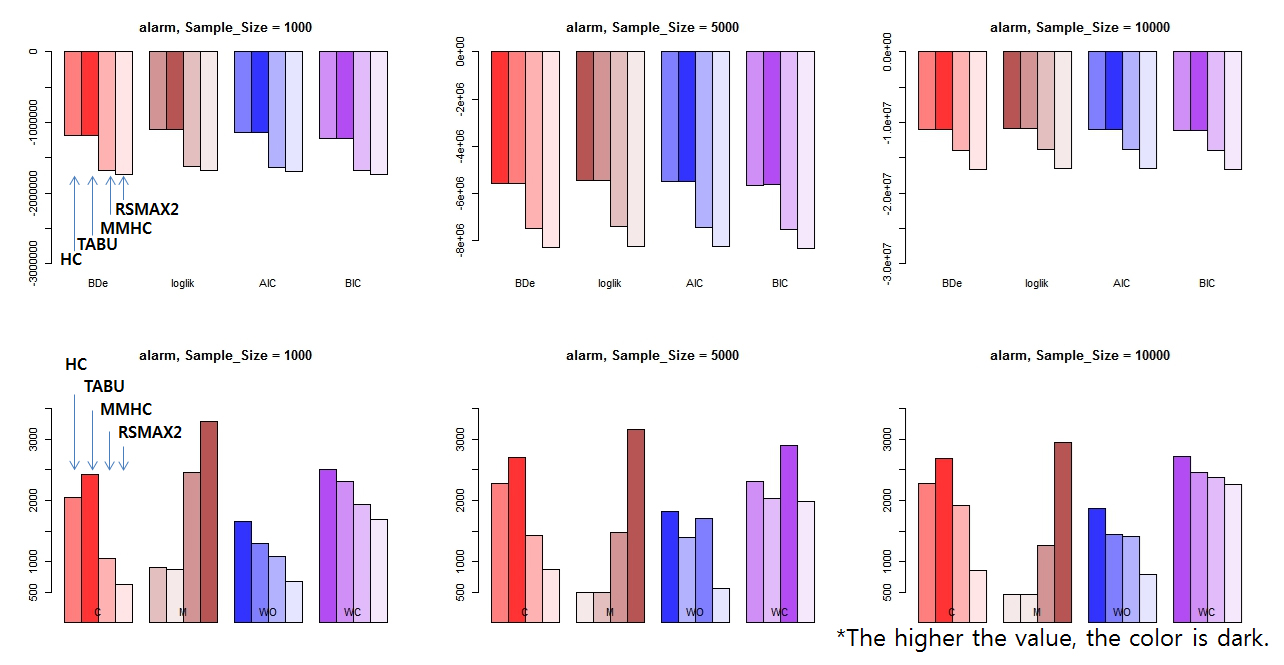
\includegraphics[height=220pt]{images/Real_3_Alarm}
		\caption{Comparison of scores and correct arcs via Hailfinder data set}
	\end{figure}	

\newpage{}

\subsection{The HaliFinder Weather Forecast System Data Set}
	\begin{figure}[h]
	\centering
		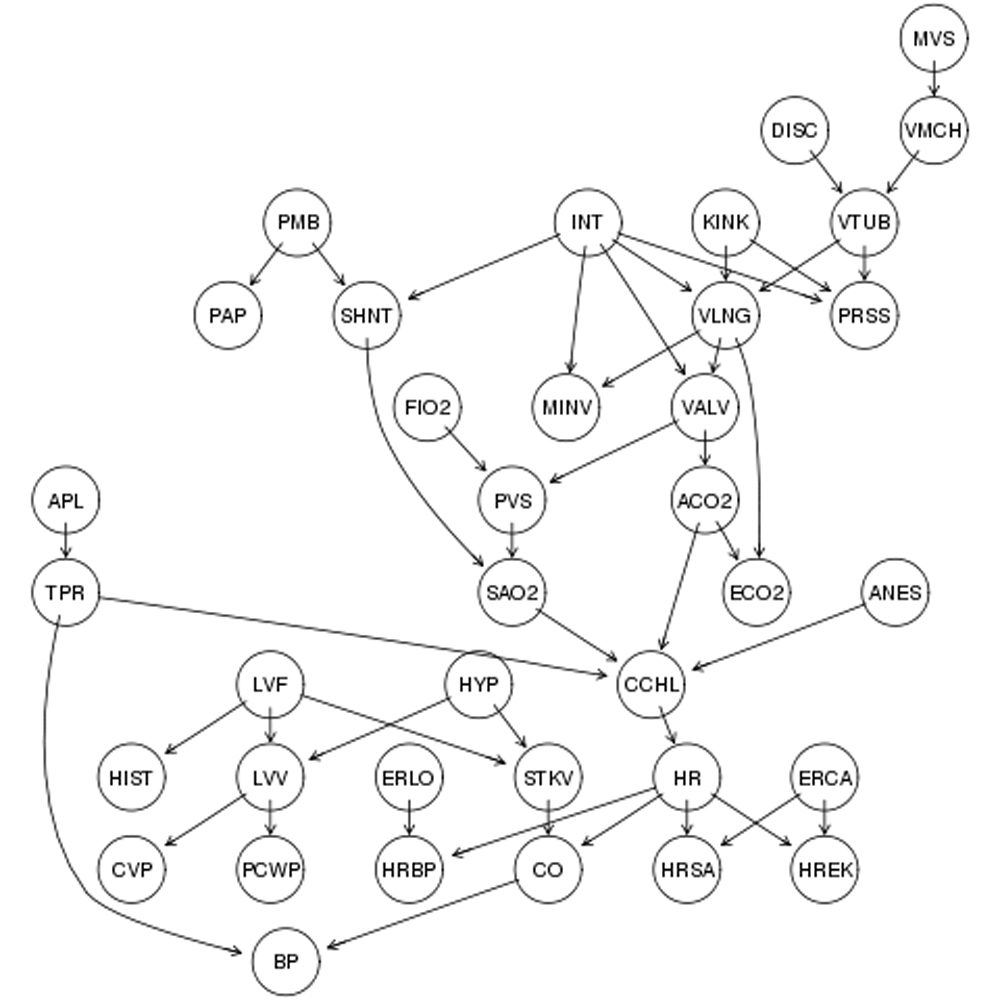
\includegraphics[height=200pt]{images/Real_Halifinder}
		\caption{Bayesian network model of The HailFinder Weather Forecast System Data Set}
	\end{figure}	

\begin{description}
	\item[Description] Hailfinder is a Bayesian network designed to forecast severe summer hail in northeastern Colorado.

	\item[Number of nodes] 56
	
	\item[Number of arcs] 66
	
	\item[Number of parameters] 2656
\end{description}

Abramson B. \emph{et al.} (1988) motivate this example. Hailfinder is a Bayesian system that combines meteorological data and models with expert judgement, based on both experience and physical understanding, to forecast severe weather in North-eastern Colorado.

% Halifinder
\begin{table}[p]																										
\centering	\caption{Comparison of scores and correct arcs via Hailfinder data set}	\tiny																						
{\tabcolsep=0.01in																										
\begin{tabular}{cc||cc|cc|cc||cc|cc|cc|cc}																										
\hline																										
&	&	\multicolumn{14}{c}{Hailfinder	(Num	of	Nodes	=	56)}\tabularnewline																			
\hline																										
\multicolumn{2}{c||}{Sample	Size}	&	\multicolumn{2}{c|}{1000}	&	\multicolumn{2}{c|}{5000}	&	\multicolumn{2}{c||}{10000}	&	&	&	\multicolumn{2}{c|}{1000}	&	\multicolumn{2}{c|}{5000}	&	\multicolumn{2}{c}{10000}\tabularnewline											
\hline																										
&	&	Sum.	&	Std.Dev.	&	Sum.	&	Std.Dev.	&	Sum.	&	Std.Dev.	&	&	&	Sum.	&	Std.Dev.	&	Sum.	&	Std.Dev.	&	Sum.	&	Std.Dev.\tabularnewline
\hline																										
\hline																										
\multirow{4}{*}{BDe} & HC &	-11006608 & 	381.65 & 	-24975425 & 	256.04 & 	-49602871 & 	297.73 & 	\multirow{4}{*}{C} & HC &	2270 & 	0.96 & 	5301 & 	0.1 & 	5586 & 	0.6\tabularnewline													
& TABU &	-11005176 & 	380.57 & 	-24975425 & 	256.04 & 	-49595842 & 	296.18 & 	& TABU &	2686 & 	1.26 & 	5301 & 	0.1 & 	5473 & 	0.8\tabularnewline													
& MMHC &	-13885378 & 	7417.41 & 	-28286426 & 	1564.45 & 	-56127215 & 	2369.94 & 	& MMHC &	1925 & 	3.09 & 	3247 & 	0.78 & 	3421 & 	1.03\tabularnewline													
& RSMAX2 &	-16586602 & 	3307.55 & 	-30165661 & 	4750.83 & 	-60211607 & 	10590.78 & 	& RSMAX2 &	858 & 	1.19 & 	2513 & 	1.45 & 	2599 & 	1.27\tabularnewline													
\hline																										
\multirow{4}{*}{loglik} & HC &	-10860805 & 	370.7 & 	-24580625 & 	264.37 & 	-49103216 & 	318.52 & 	\multirow{4}{*}{M} & HC &	468 & 	0.69 & 	1299 & 	0.1 & 	974 & 	0.52\tabularnewline													
& TABU &	-10861471 & 	371.47 & 	-24580625 & 	264.37 & 	-49101011 & 	318.75 & 	& TABU &	468 & 	0.69 & 	1299 & 	0.1 & 	975 & 	0.52\tabularnewline													
& MMHC &	-13790813 & 	7449.01 & 	-28061042 & 	1631.98 & 	-55832193 & 	2457.02 & 	& MMHC &	1268 & 	1.56 & 	3350 & 	0.78 & 	3179 & 	1.03\tabularnewline													
& RSMAX2 &	-16508716 & 	3325.33 & 	-30028409 & 	4793.11 & 	-60050894 & 	10637.32 & 	& RSMAX2 &	2949 & 	1.05 & 	4086 & 	1.44 & 	4001 & 	1.27\tabularnewline													
\hline																										
\multirow{4}{*}{AIC} & HC &	-10923175 & 	374.81 & 	-24722989 & 	261.22 & 	-49264998 & 	310.85 & 	\multirow{4}{*}{WO} & HC &	1862 & 	0.9 & 	0 & 	0 & 	40 & 	0.49\tabularnewline													
& TABU &	-10921249 & 	372.87 & 	-24722989 & 	261.22 & 	-49262249 & 	308.38 & 	& TABU &	1446 & 	1.27 & 	0 & 	0 & 	152 & 	0.58\tabularnewline													
& MMHC &	-13816106 & 	7435.45 & 	-28135869 & 	1609.27 & 	-55920440 & 	2432.1 & 	& MMHC &	1407 & 	1.98 & 	3 & 	0.17 & 	0 & 	0\tabularnewline													
& RSMAX2 &	-16527481 & 	3318.41 & 	-30070905 & 	4758.8 & 	-60096326 & 	10600.54 & 	& RSMAX2 &	793 & 	0.71 & 	1 & 	0.1 & 	0 & 	0\tabularnewline													
\hline																										
\multirow{4}{*}{BIC} & HC &	-11148029 & 	416.51 & 	-25186896 & 	253.21 & 	-49848249 & 	291.84 & 	\multirow{4}{*}{WC} & HC &	2714 & 	1.56 & 	1016 & 	0.55 & 	1028 & 	0.75\tabularnewline													
& TABU &	-11136759 & 	427.99 & 	-25186896 & 	253.21 & 	-49843539 & 	288.2 & 	& TABU &	2452 & 	2.25 & 	1016 & 	0.55 & 	1112 & 	1.08\tabularnewline													
& MMHC &	-13907292 & 	7386.76 & 	-28379700 & 	1538.4 & 	-56238585 & 	2345.93 & 	& MMHC &	2368 & 	2.84 & 	1424 & 	2.67 & 	1662 & 	2.16\tabularnewline													
& RSMAX2 &	-16595132 & 	3293.99 & 	-30209383 & 	4647.37 & 	-60260116 & 	10468.63 & 	& RSMAX2 &	2262 & 	1.96 & 	166 & 	1.36 & 	132 & 	1.07\tabularnewline													
\hline																										
\end{tabular}																										
}																										
\end{table}

	\begin{figure}[p]
	\centering
		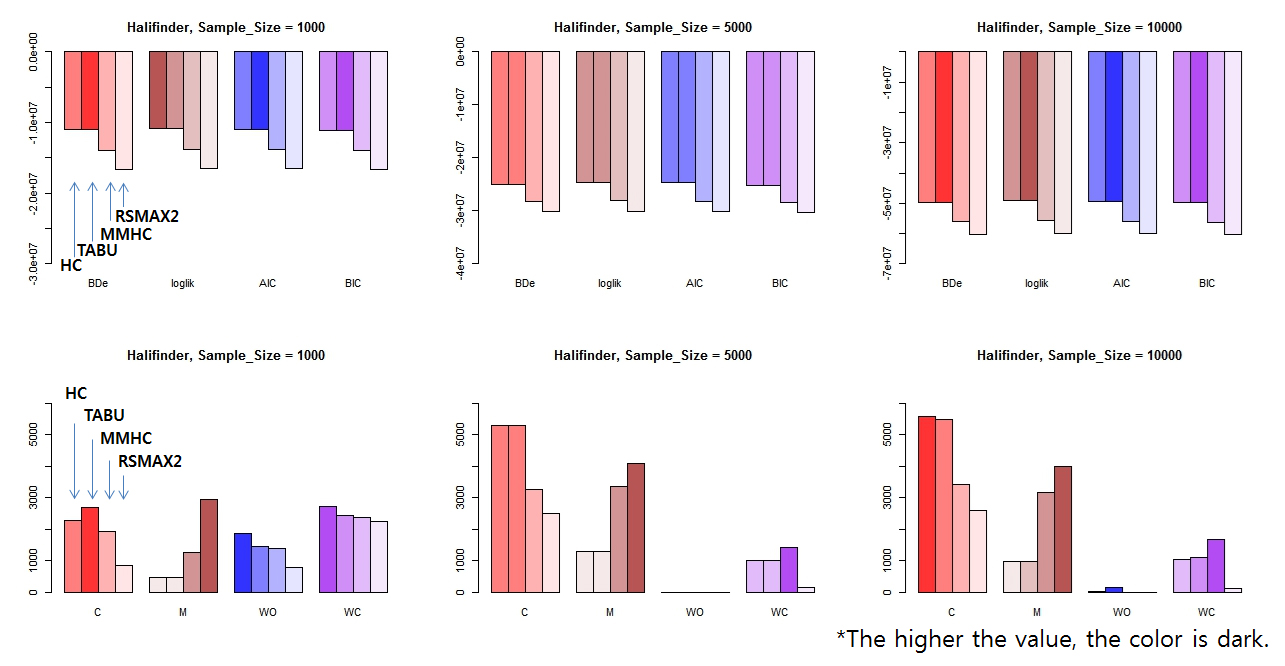
\includegraphics[height=220pt]{images/Real_4_Halifinder}
		\caption{Comparison of scores and correct arcs via Hailfinder data set}
	\end{figure}	

\newpage{}

\subsection{Summary}
	\begin{figure}[!h]
	\centering
		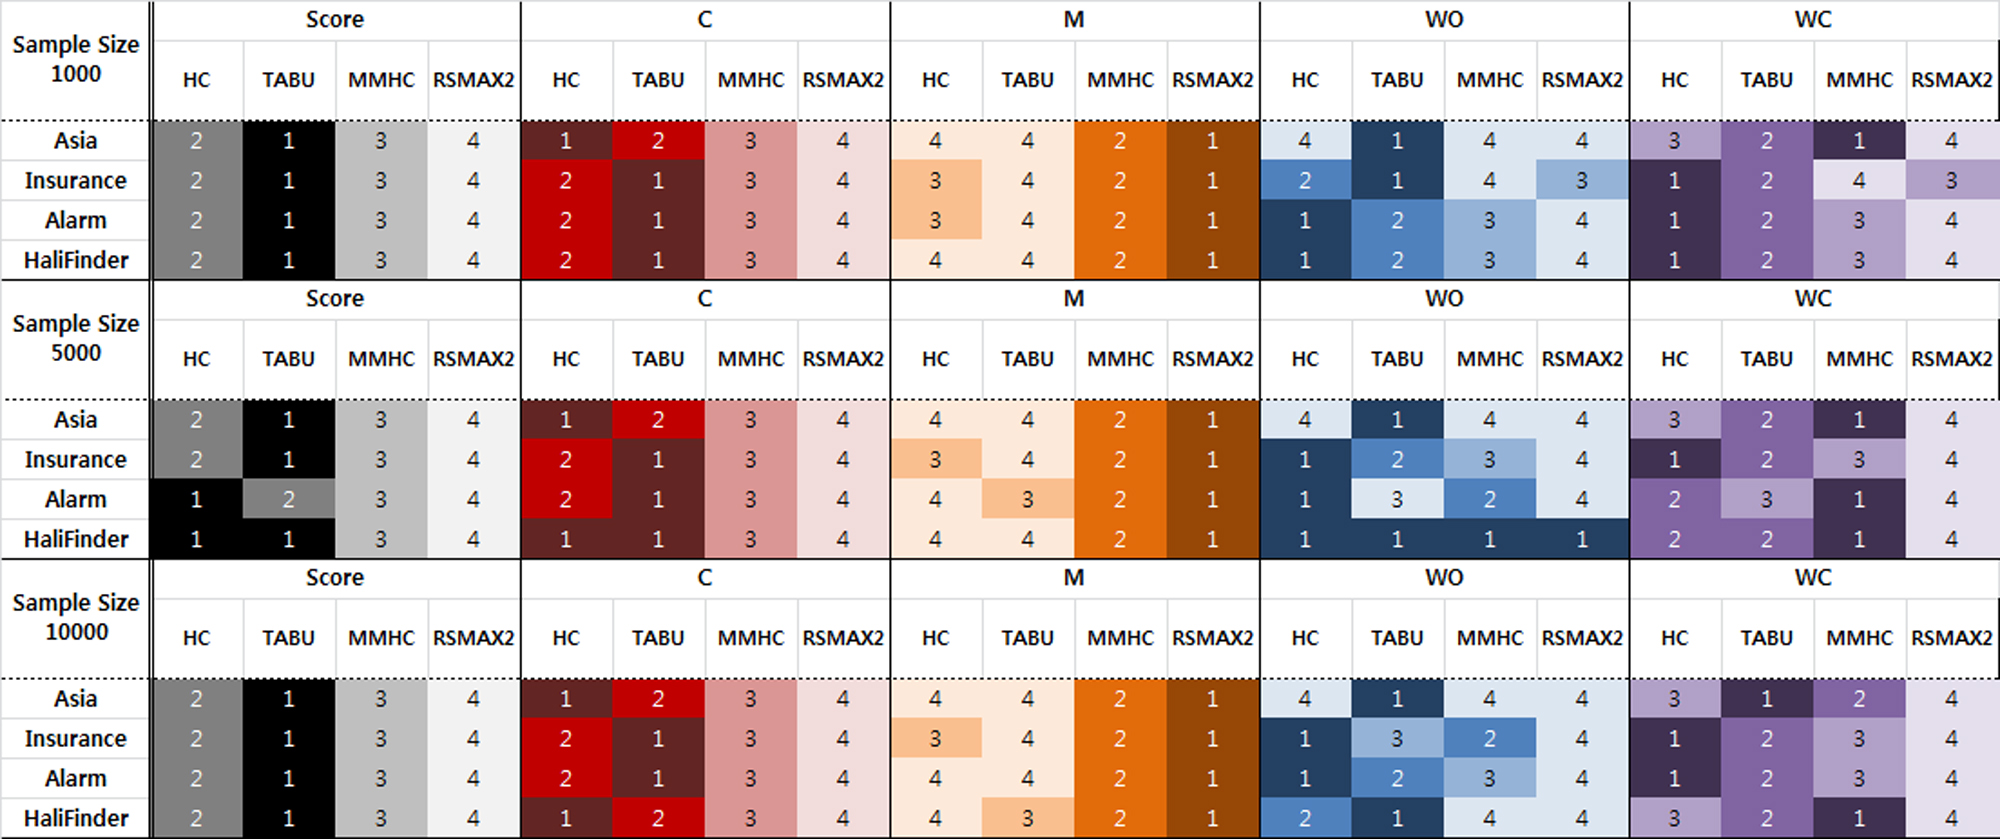
\includegraphics[height=170pt]{images/Real_Result}
		\caption{Summary for Comparison of scores and correct arcs via real data sets}
	\end{figure}	

% Score를 기준으로 비교했을 때는, 대부분 TABU search 알고리즘, Hill-Climbing 알고리즘 순으로 좋은 성능을 나타내는 것으로 나타났다.
When compared to the Score criteria were found to show good performance most TABU search algorithm, the order of Hill-Climbing algorithm.

% 그러나 목표 네트워크와 학습 네트워크를 직접 비교한 결과는 조금 달랐다.
However, as a result of comparing the target network and learning network directly, was a little different.

% 목표 네트워크와 학습 네트워크를 직접 비교한 결과는 C가 많을 때, 그리고 M, WO, WC가 적을 때 성능이 좋다고 이야기할 수 있다.
Result of comparing the target network and learning network directly, when C is large, M, WO, it can be said that performance is better when the WC is small.

% TABU search 알고리즘이, C의 개수도 여전히 많은 편이었지만, score 기준으로 봤을 때 다른 알고리즘에 비해 압도적인 성능이었던 것을 감안하면 다소 실망스럽다. 오히려 WO, WC의 개수도 많은 편이어서, 화살표의 방향이 어긋나거나, 엉뚱한 화살표가 그려지는 것이 단점으로 평가된다.
TABU search algorithm, but were still many number of C, when it is a score criterion, considering that was overwhelming performance than other algorithms, it has been somewhat disappointing. Because rather WO, also the number of WC large, or shift the direction of the arrow, that unreasonable arrow is drawn is evaluated as disadvantages.

% MMHC, RSMAX2는 C도 적고 M도 많지만, WO, WC도 적은 것으로 나타났다. 전반적으로 화살표 개수가 Hill-climbing, TABU search에 비해 적게 그려지는 것이다. 이는 MMHC, RSMAX2와 같은 Hybrid 알고리즘이, Score-Based 알고리즘에 비해 학습 과정에서 화살표를 보수적으로 이어준다는 것을 확인할 수 있는 결과이다.
MMHC, RSMAX2 but C is also less M many, WO, I found that WC is also small. Overall the number of arrows Hill-climbing, will be drawn smaller than the TABU search. This Hybrid algorithms such as MMHC, RSMAX2 is, in the learning process in comparison with the Score-Based Algorithm, is the result that it can be confirmed that that will conservatively subsequently arrow.

% 모형의 형태가 다르기 때문에 이들을 이용하여 node 개수에 따른 알고리즘 성능 비교는 곤란하다. 또한 sample size가 커짐에 따른 변화도 뚜렷한 것은 발견하기 어렵다.
Since the shape of the model is different, by using them, performance comparison of the algorithm according to the node number is difficult. Also, it is difficult to discover that the sample size is also clear changes in accordance with the increase.

\newpage{}

% Synthetic Data
\section{Synthetic Data According to Topologies}

\subsection{Bayesian Network Topologies}
	\begin{figure}[!h]
	\centering
		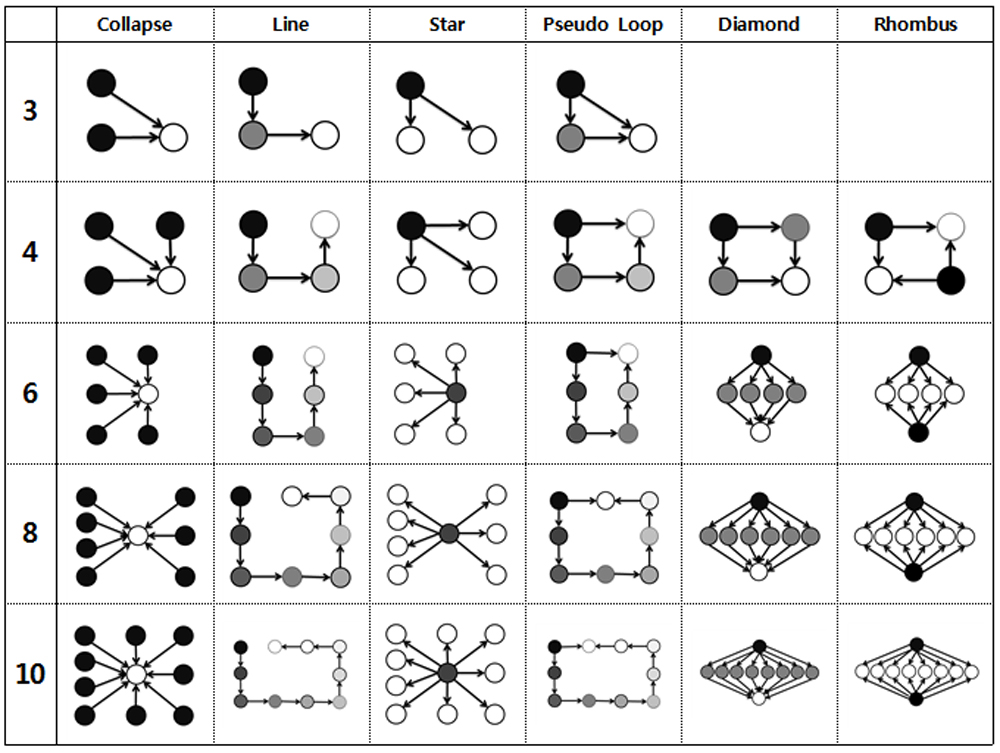
\includegraphics[height=180pt]{Topologies}
		\caption{Bayesian Networks with varying topologies and number of nodes}
	\end{figure}

% 베이지안 네트워크 모형은 노드의 개수가 많아질수록, 그 모형의 어떠한 규칙을 정확히 말하기 어려워진다. 대신 그 모형이 변형됨에도 불구하고 변하지 않는 일정한 성질을 지닌 topology별로 나누어 볼 수 있다. Eitel(2008)은 베이지안 네트워크의 topology를 구분하는 시도를 하였다.
Bayesian network model, as the number of nodes increases, difficult speaking any rules of the model accurately. Instead, even though the model is deformed, topology can be viewed separately separately with a certain properties unchanged. Eitel (2008) was trying to distinguish topology of Bayesian network.

% 여기에서는 이 topology에 따라, 노드 개수를 3, 4, 6, 8, 10개 까지 정하여 모형을 생성한 뒤, 그 모형에 대한 모의 실험을 진행하였다. Cardinality는 2로 제한되었다. 즉 모든 변수는 binary data이다. 확률 값은 $U(0, 1)$의 분포 하에서 임의로 부여하였으며, 우연에 의해 결과가 치우치는 경우를 최소화하기 위해, 모든 실험은 100번 반복한 뒤 그 결과의 합과 표준편차를 계산하였다.
Here, depending on the topology, after creating a set of models of the number of nodes to 3, 4, 6, 8, 10 pieces, we simulate the model. Cardinality was limited to two. In other words, all of the variable is the binary data. The probability value, which is imparted optionally under $ U (0,1) $ distribution. And in order to avoid the influence of chance, all experiments are repeated 100 times, and overall results.

\newpage{}

\subsection{Collapse}
	\begin{figure}[!bhp]
	\centering
		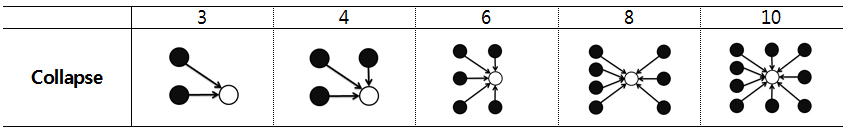
\includegraphics[height=50pt]{Topologies_Collapse}
		\caption{Bayesian Network Topology : Collapse}
	\end{figure}	

	% Collapse는 한 개의 자식 node에 여러 개의 부모 노드가 존재하는 형태이다.
	Collapse is a form in which a plurality of parent nodes are present in one child node.

	\begin{figure}[!bhp]
	\centering
		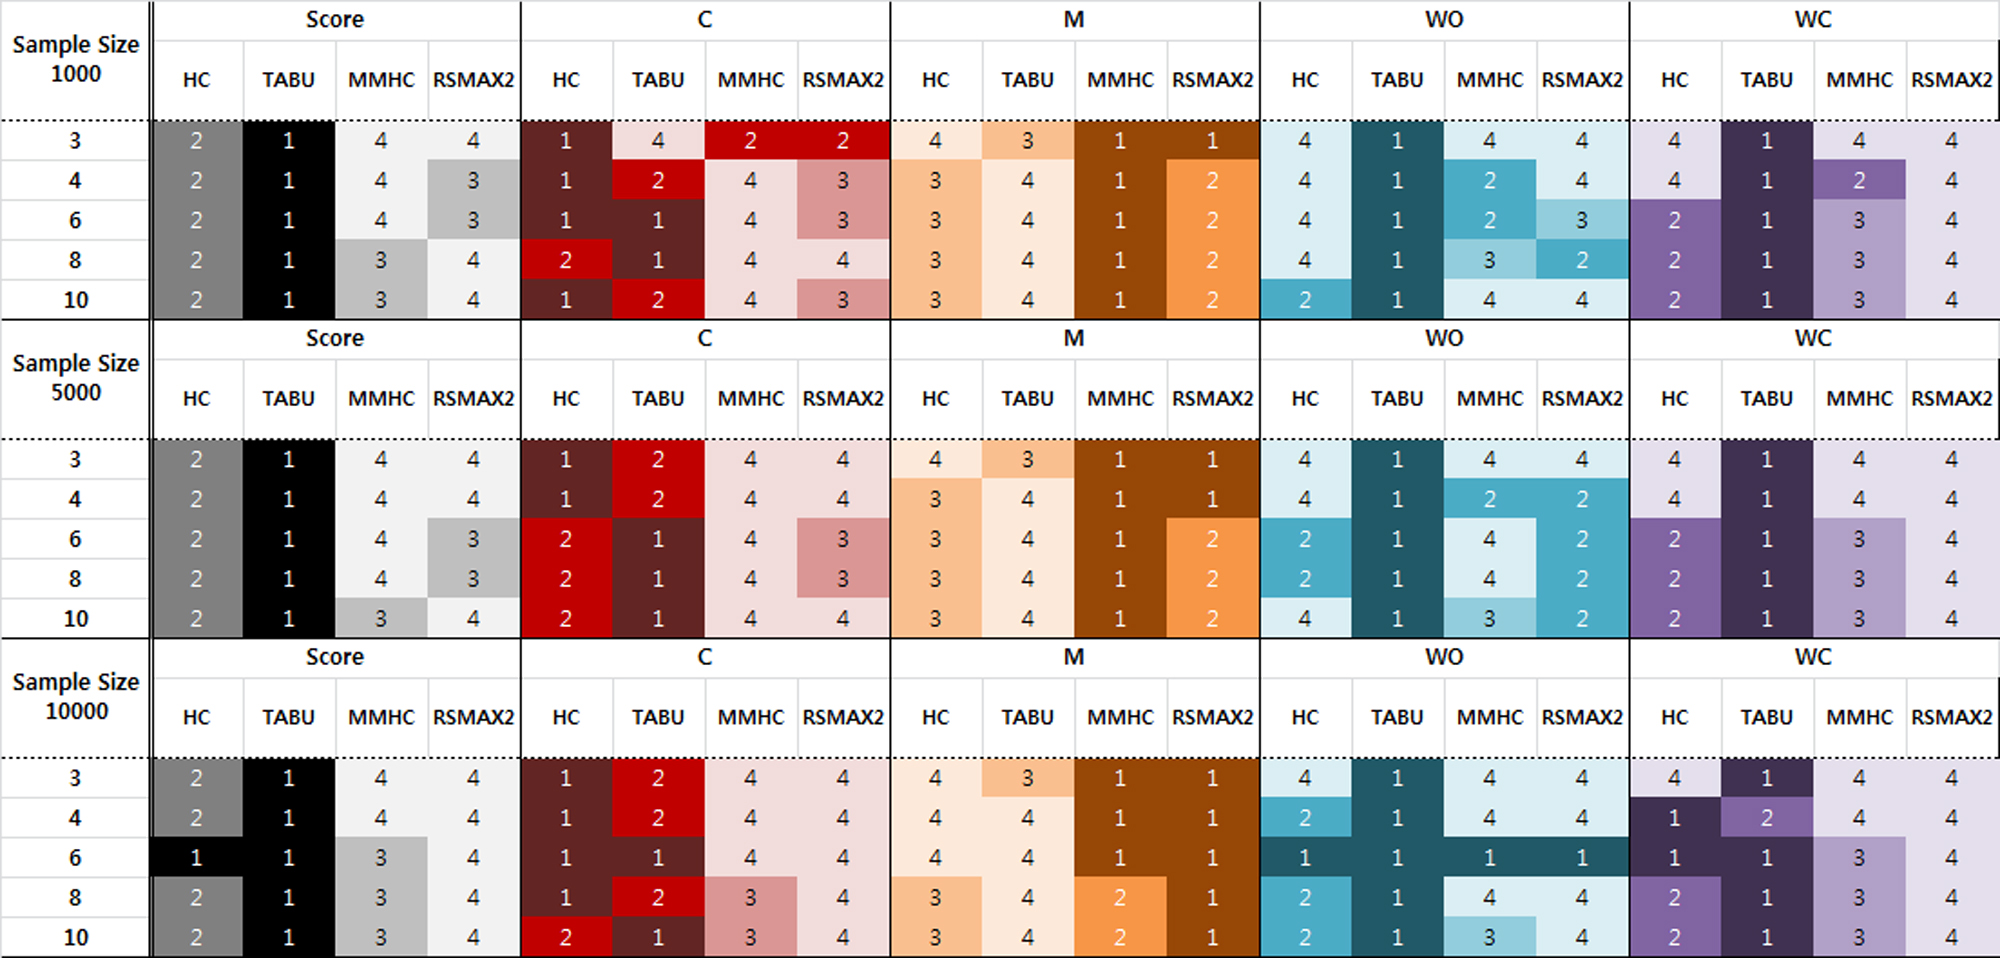
\includegraphics[height=170pt]{Result_Collapse}
		\caption{Summary for Comparison via Collapse}
	\end{figure}	
	
% Real data set을 이용하여 분석할 때와 마찬가지로, score를 기준으로 하였을 때 TABU search 알고리즘, Hill-climbing 알고리즘 순으로 성능이 좋은 것으로 나타났다.
The same way that you were analyzed using the Real data set, TABU search algorithm when it is on the basis of the score, in the order of the Hill-climbing algorithm performance is found to be good.

% 그러나 C의 개수는 TABU search와 Hill-climbing이 서로 경합을 벌였다. 오히려 TABU search의 경우 WO, WC의 개수가 많이 나타났다.
However, the number of C is, TABU search and Hill-climbing has been engaged in a conflict with each other. Rather the case of TABU search WO, became a lot number of WC.

% Hill-climbing의 경우 TABU search만큼은 아니지만, node의 개수가 많아질수록, sample size가 커질수록 WO의 개수가 많아지는 현상이 나타났다.
Not as much as TABU search case of Hill-climbing, The more the number of node, sample size appeared many made phenomenon is the number of larger the WO.

% MMHC는 sample size가 커질수록 missing이 줄어드는 반면, RSMAX2는 오히려 늘어나는 현상이 나타났다.
MMHC While sample size decreases the larger the missing, RSMAX2 increases phenomenon appeared rather.
	
	\begin{figure}[p]
	\centering
		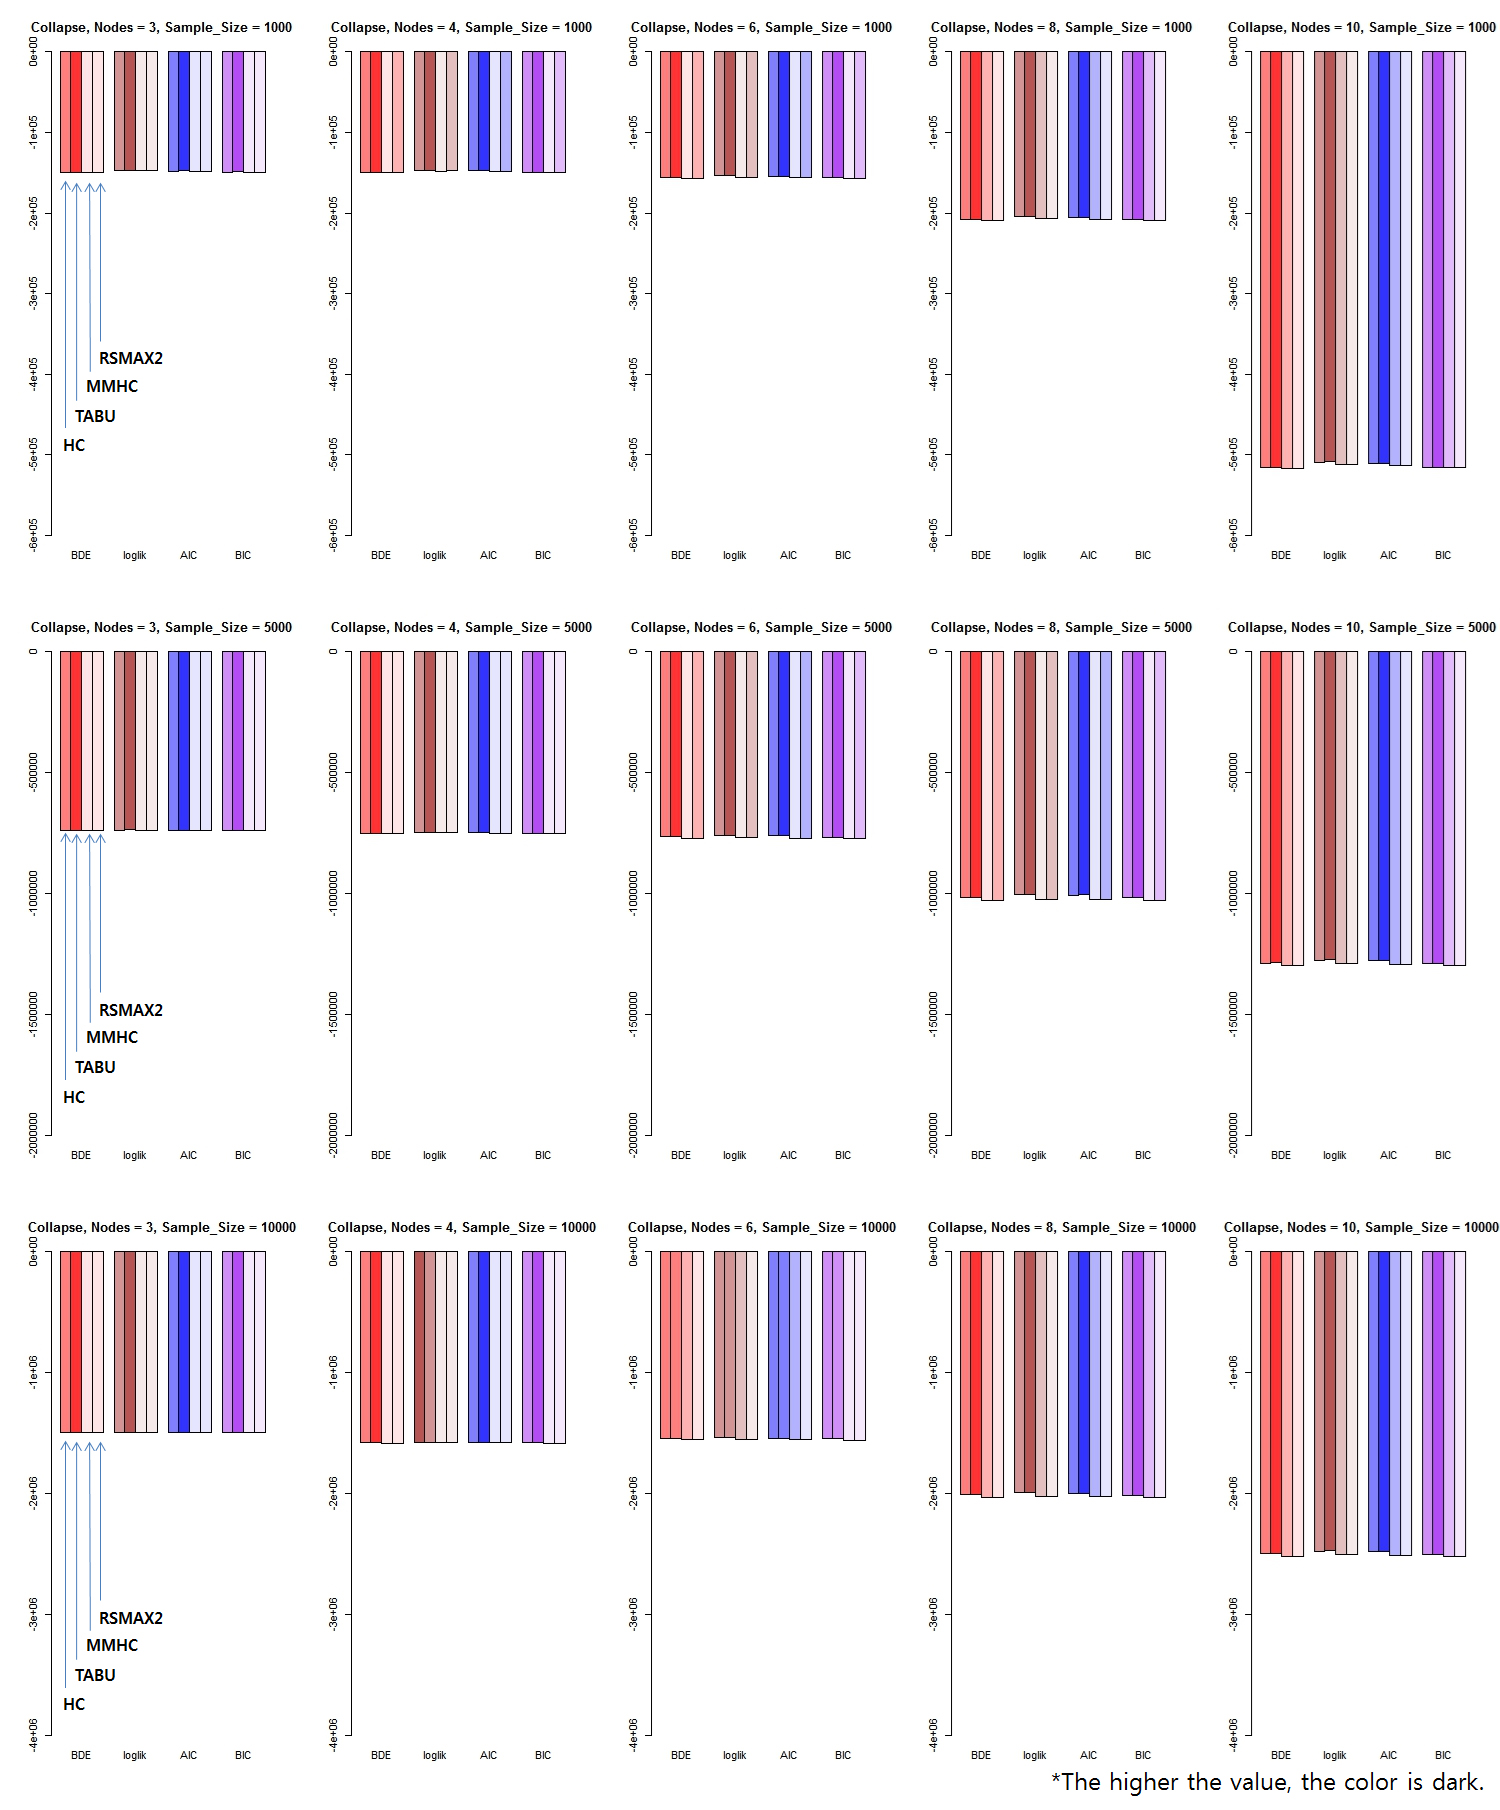
\includegraphics[height=500pt]{01_Collapse_Score}
		\caption{Comparison of scores via Collapse}
	\end{figure}	

	\begin{figure}[p]
	\centering
		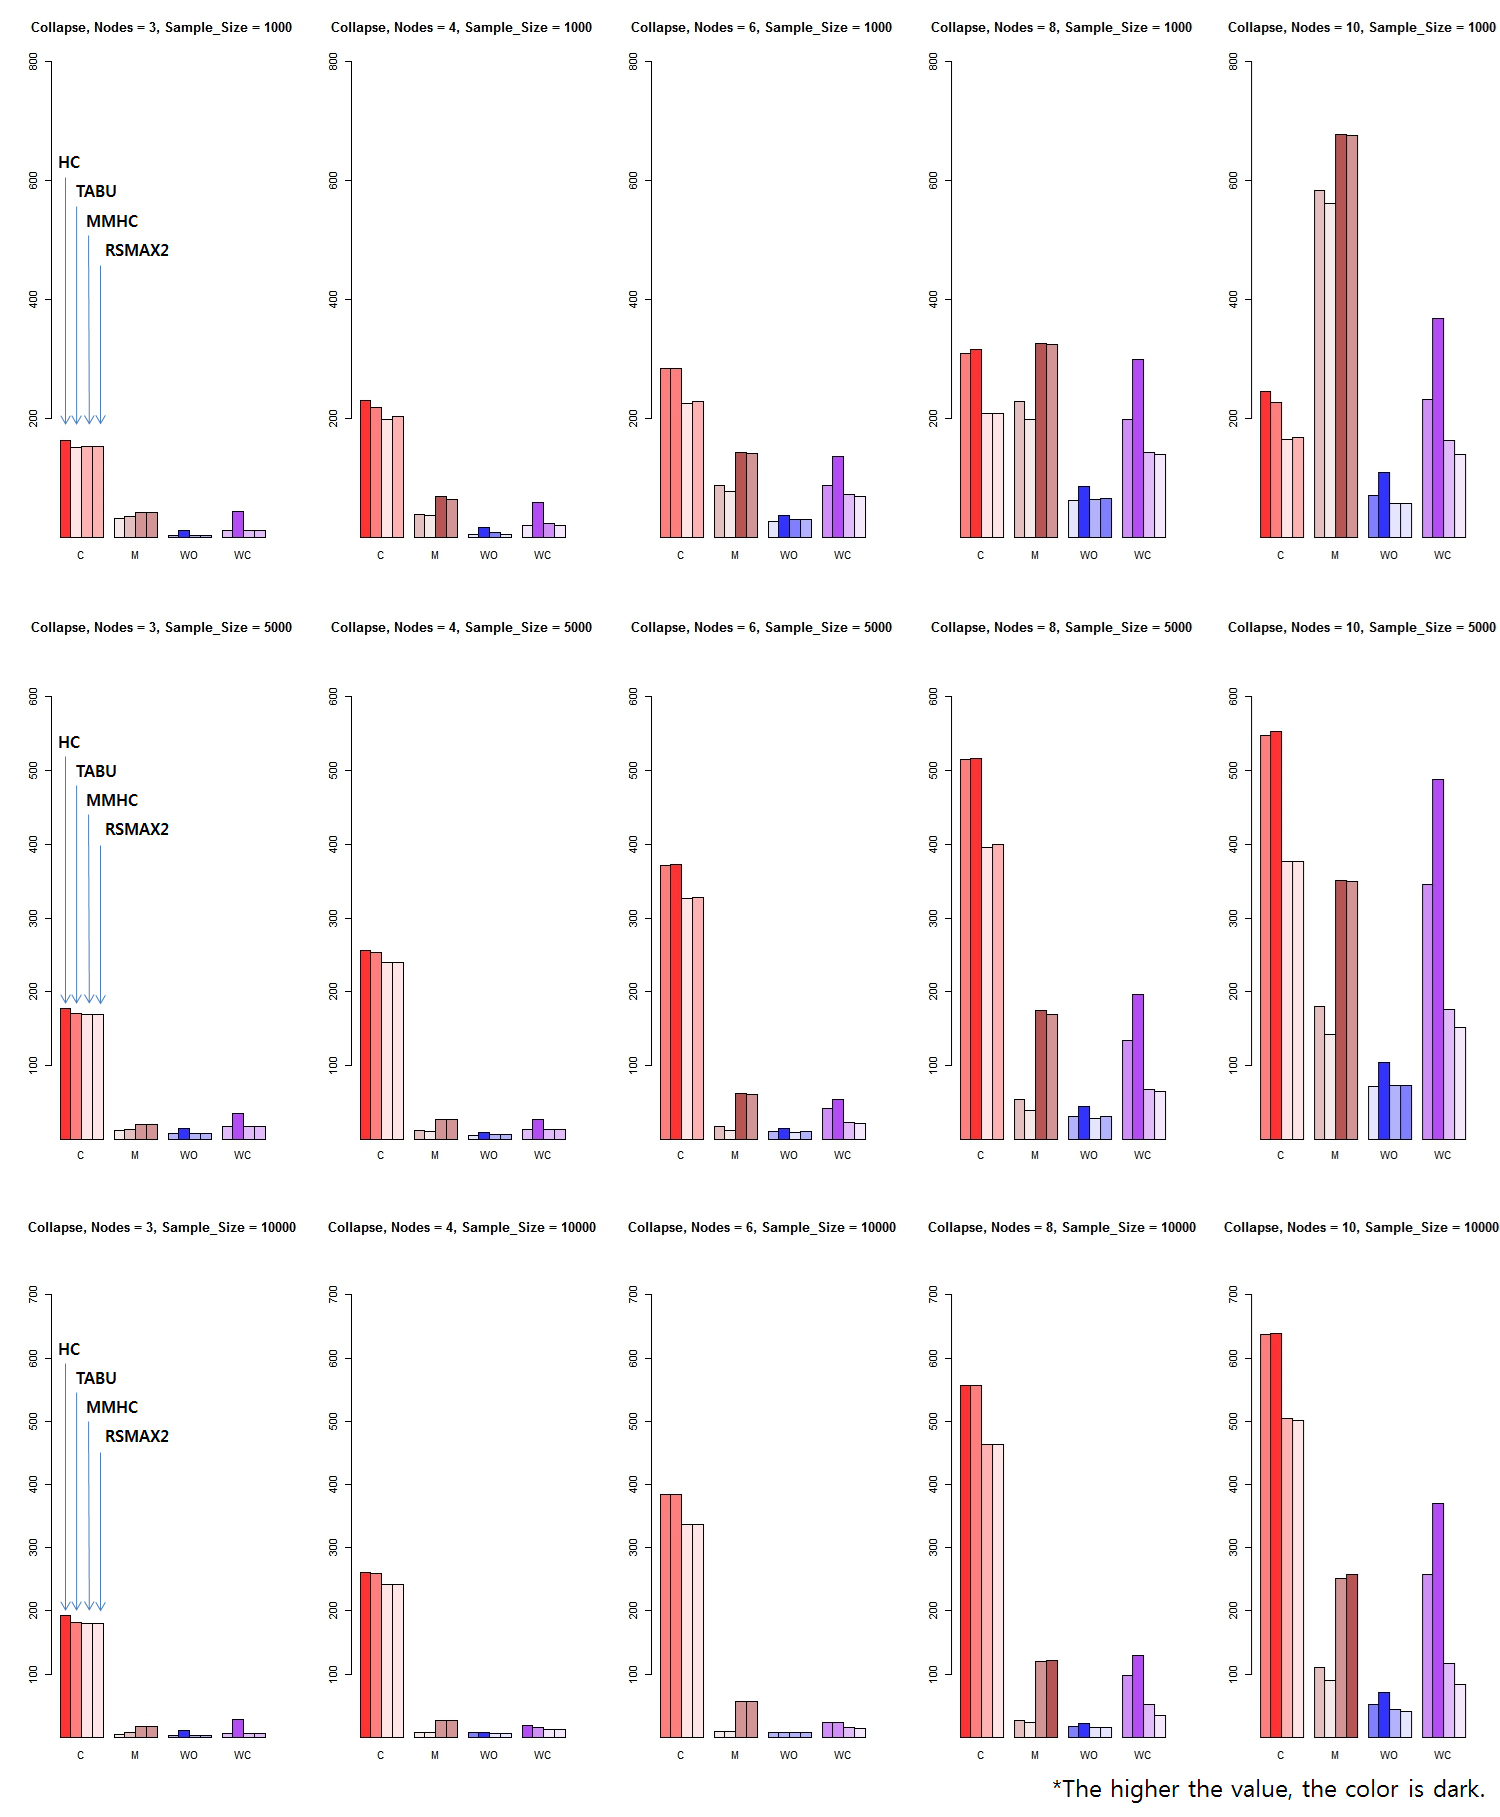
\includegraphics[height=500pt]{01_Collapse_Arcs}
		\caption{Comparison of correct arcs via Collapse}
	\end{figure}	

\newpage{}



\newpage{}

\subsection{Line}
	\begin{figure}[!bhp]
	\centering
		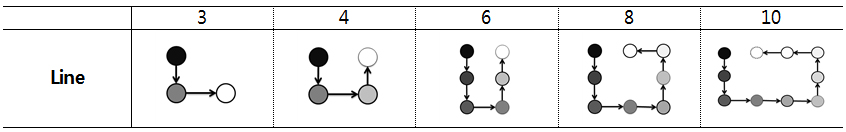
\includegraphics[height=50pt]{images/Topologies_Line}
		\caption{Bayesian Network Topology : Line}
	\end{figure}	

	% Line 형태는 자식 node의 자식 node, 또 그 자식 node가 계속 이어지는 형태를 말한다. 마치 그 모습이 line과 같다.
	Multiple node bite the tail of the tail, then this form called Line. Though the figure is as of line.

	\begin{figure}[!bhp]
	\centering
		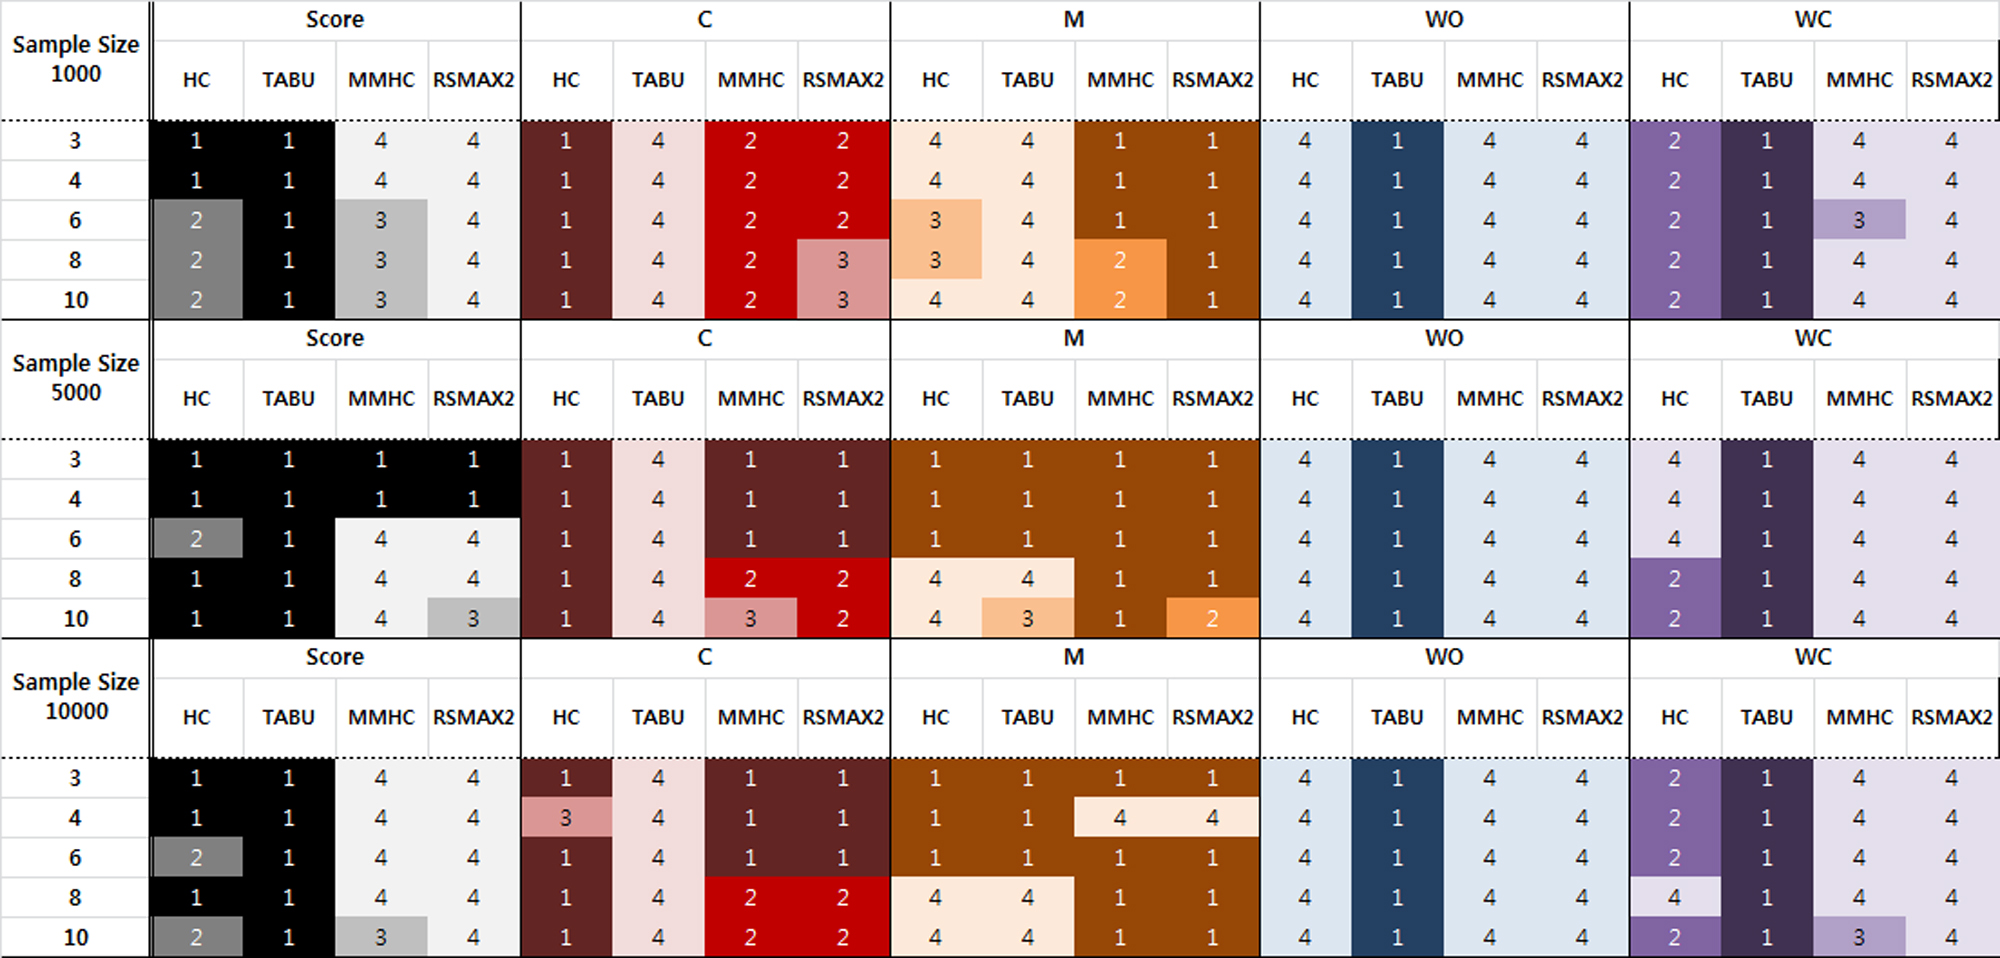
\includegraphics[height=155pt]{images/Result_Line}
		\caption{Summary for Comparison via Line}
	\end{figure}	
	
% 다른 topology에 비해 알고리즘별 성능이 크게 차이가 발생하지 않았다.
Performance of each algorithm is compared to other topology were not different significantly occurs.

% 그러나 TABU search는 score에 따른 성능이 좋음에도 불구, 다른 알고리즘에 비해 C의 개수가 압도적으로 적고, M, WO, WC의 개수가 무척 높은 모습이 나타났다.
However, TABU search, despite good performance by score, the number of C is overwhelmingly smaller than the other algorithms, and M, WO, and WC is larger than the other algorithms.

% 상대적으로 Hill-climbing이 line 형태에 대해 좋은 성능을 보여주었다.
Relatively, Hill-climbing has showed good performance for line form.

	\begin{figure}[p]
	\centering
		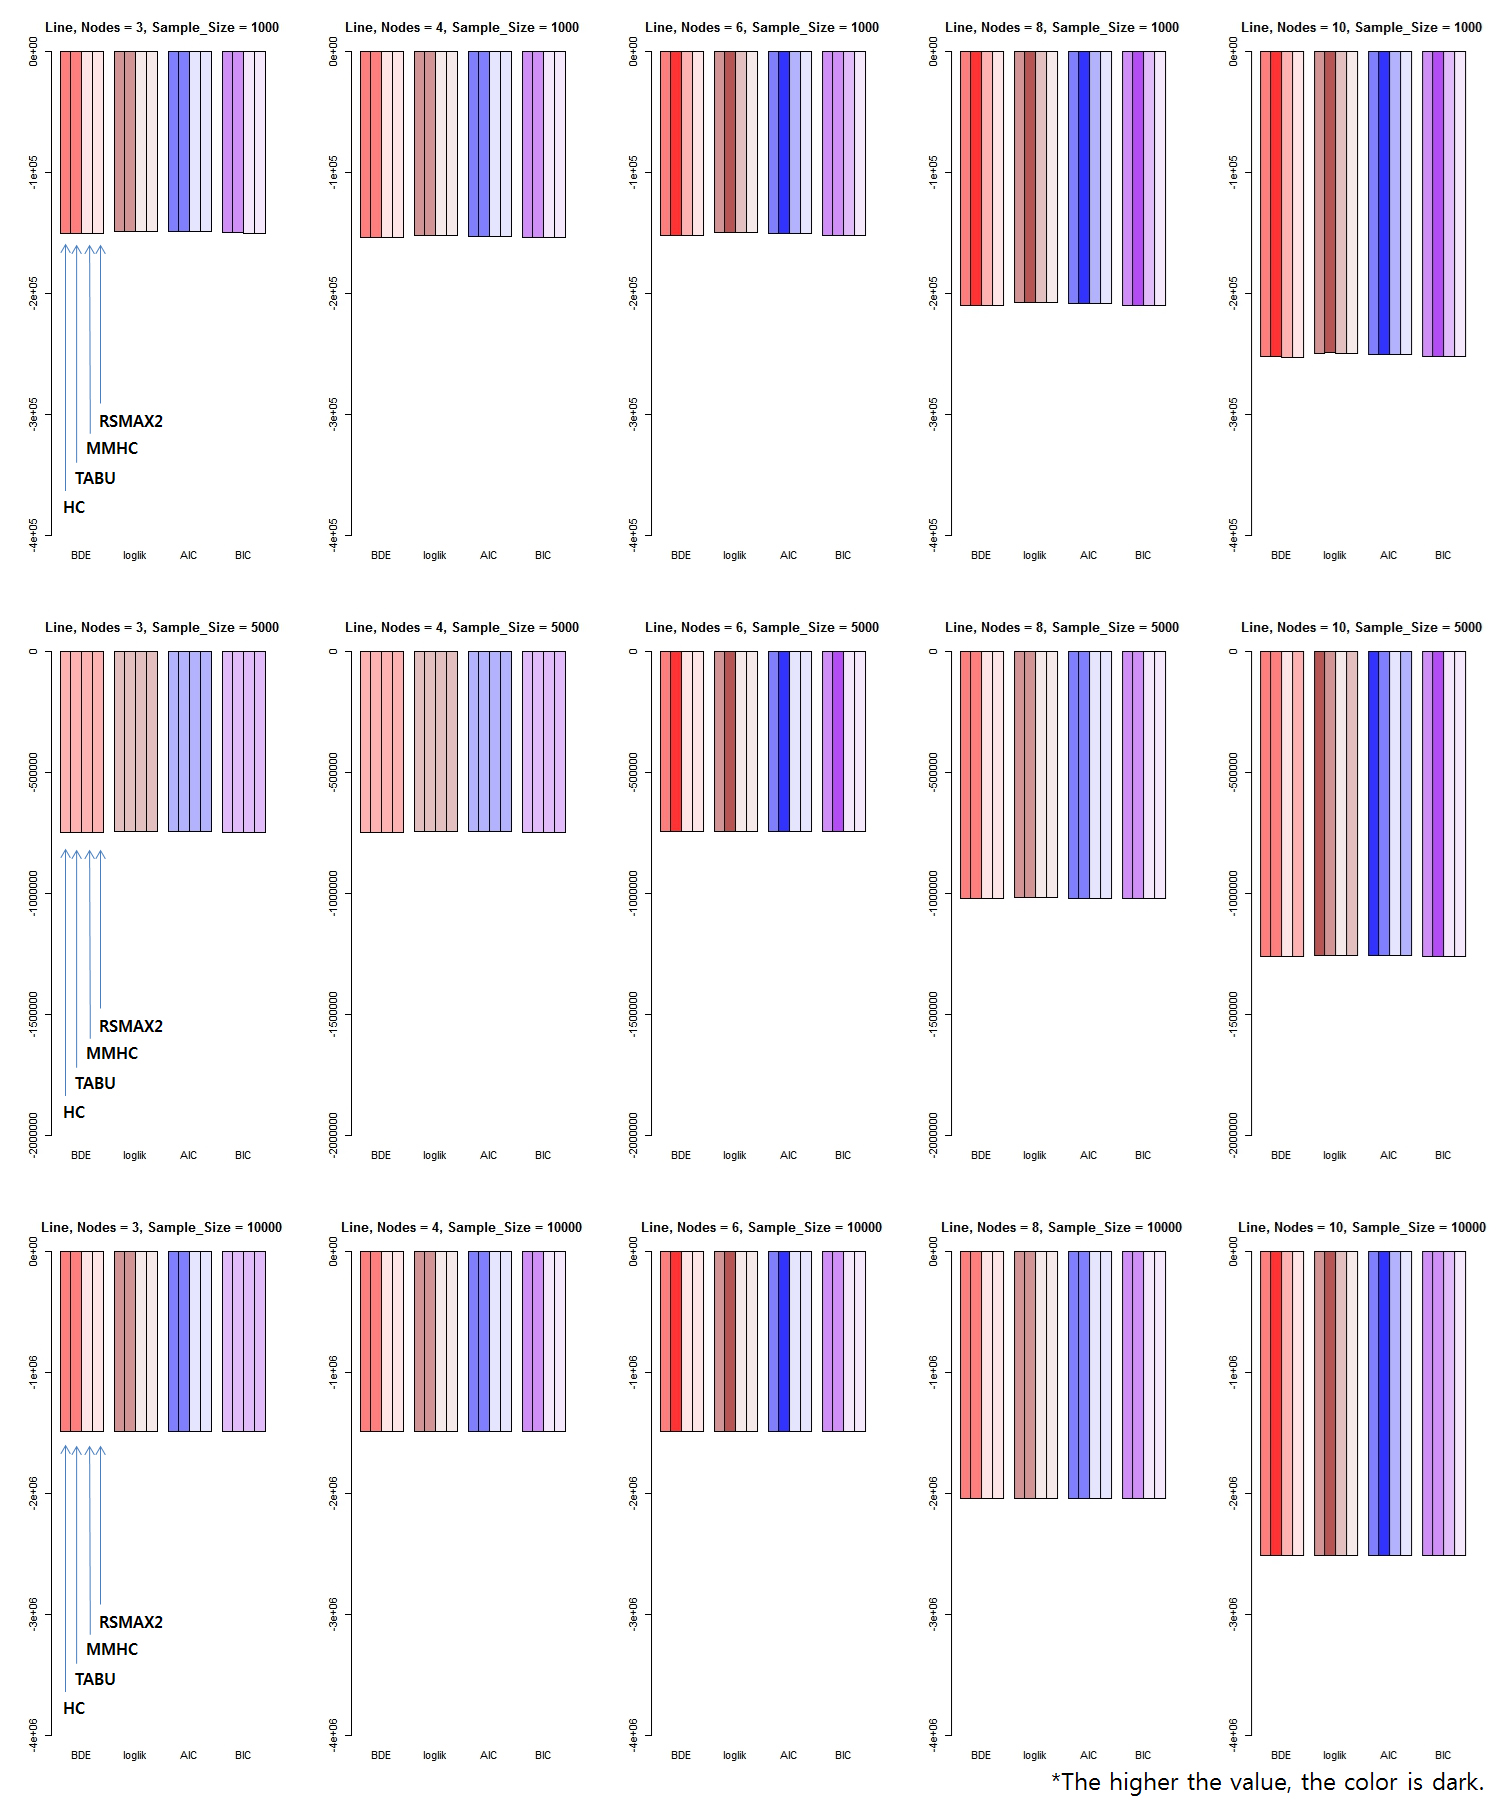
\includegraphics[height=500pt]{images/02_Line_Score}
		\caption{Comparison of scores via Line}
	\end{figure}	

	\begin{figure}[p]
	\centering
		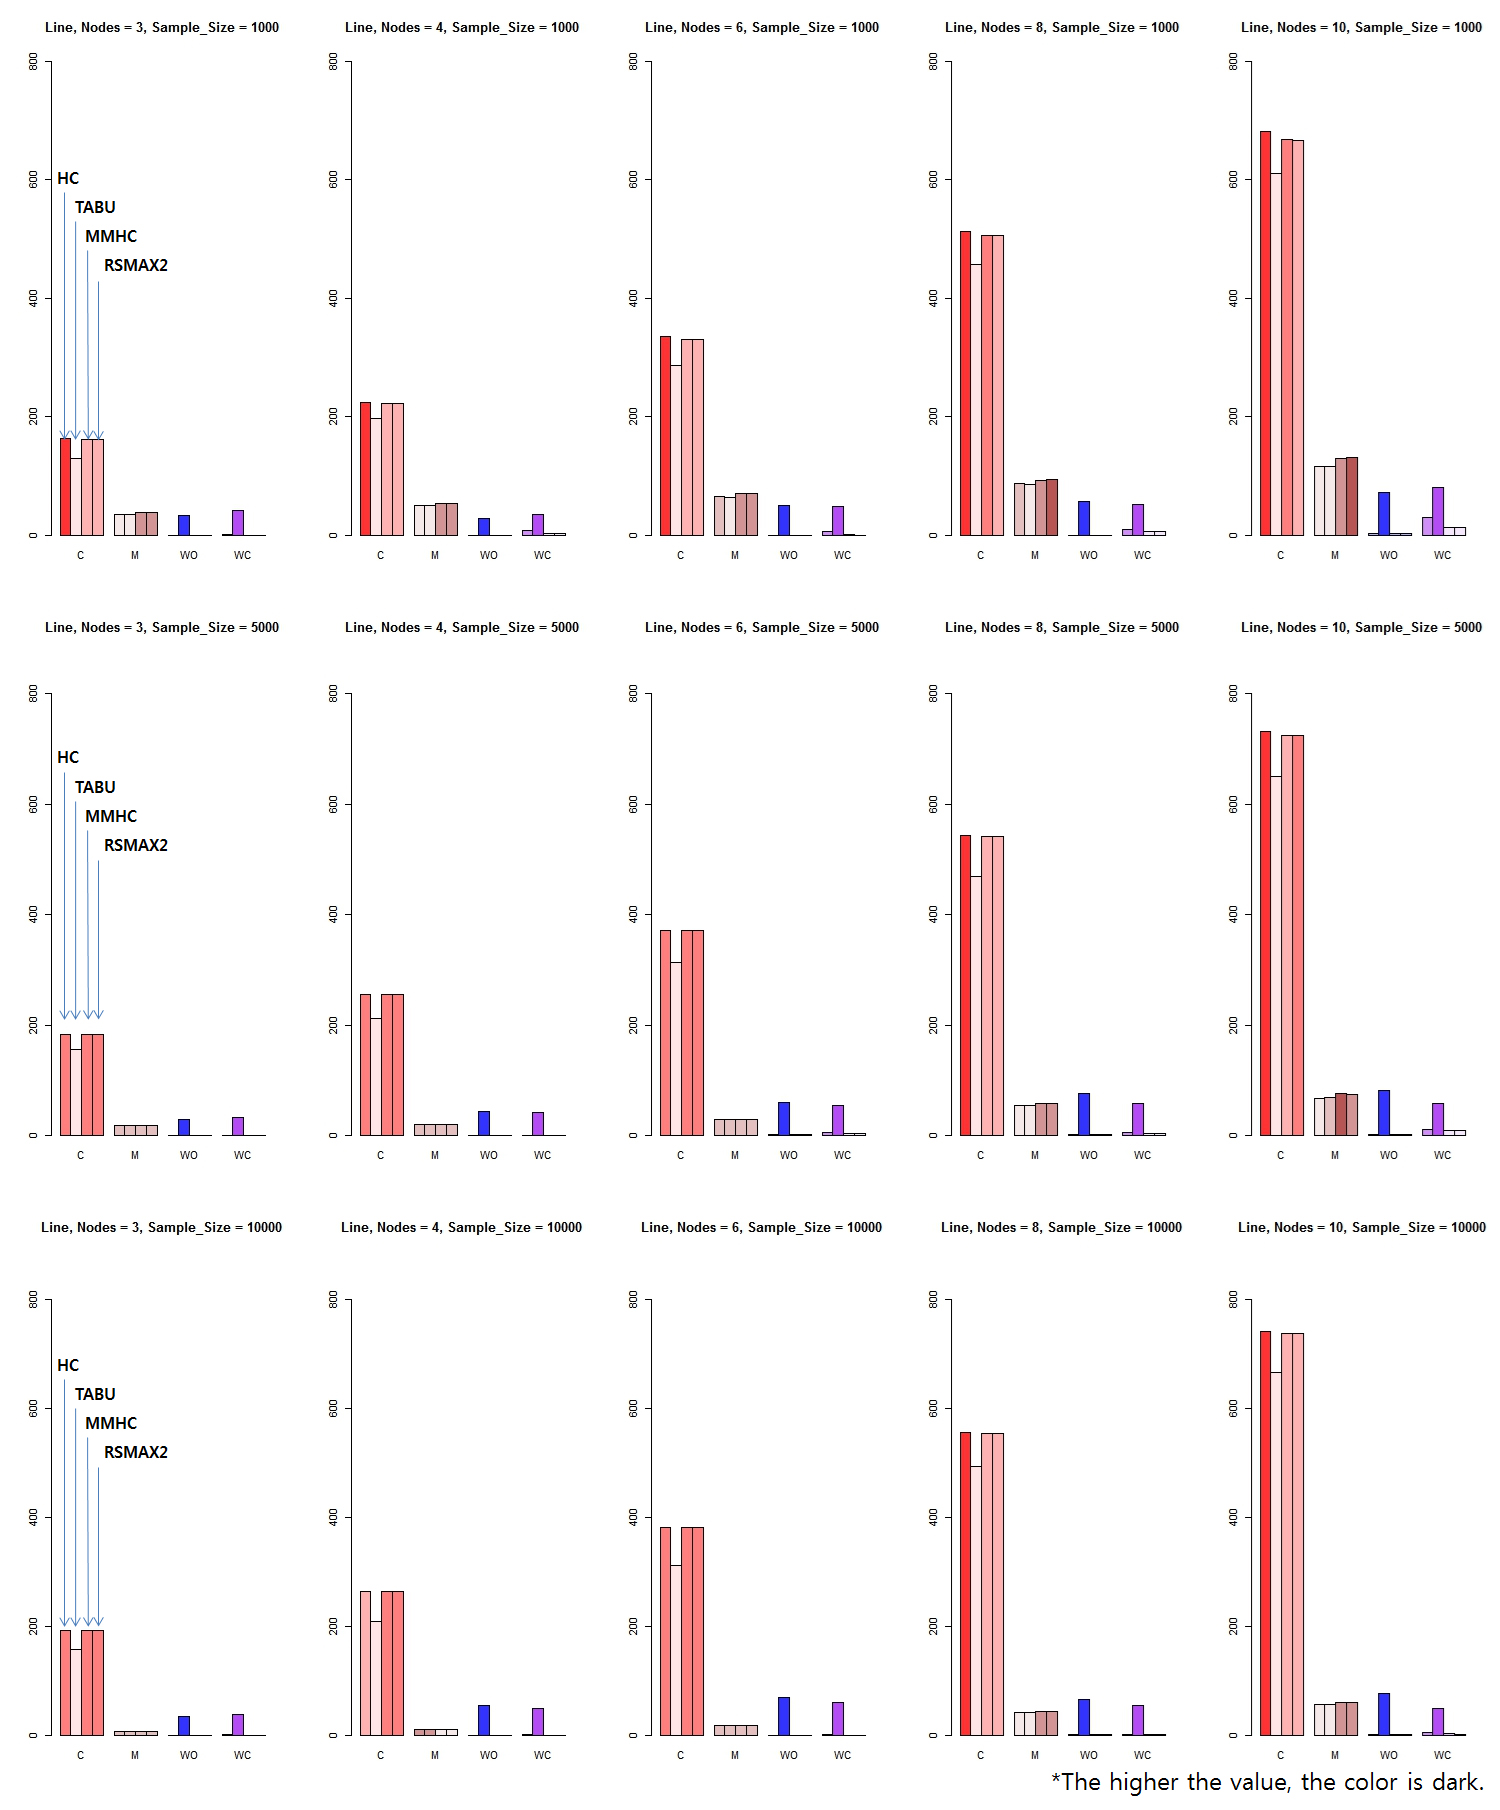
\includegraphics[height=500pt]{images/02_Line_Arcs}
		\caption{Comparison of correct arcs via Line}
	\end{figure}	


\newpage{}
	
\subsection{Star}
	\begin{figure}[h]
	\centering
		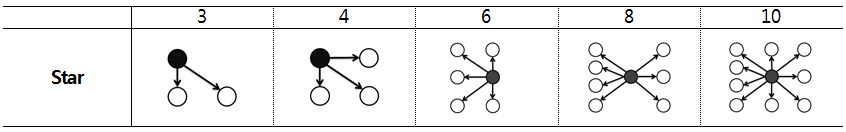
\includegraphics[height=50pt]{Topologies_Star}
		\caption{Bayesian Network Topologies : Star}
	\end{figure}	
	
	% Star 형태는 한 개의 node가 여러 개의 자식 node를 가진 형태를 말한다.
	Star forms, one node refers to a plurality of child node forms.

\begin{figure}[!bhp]
	\centering
		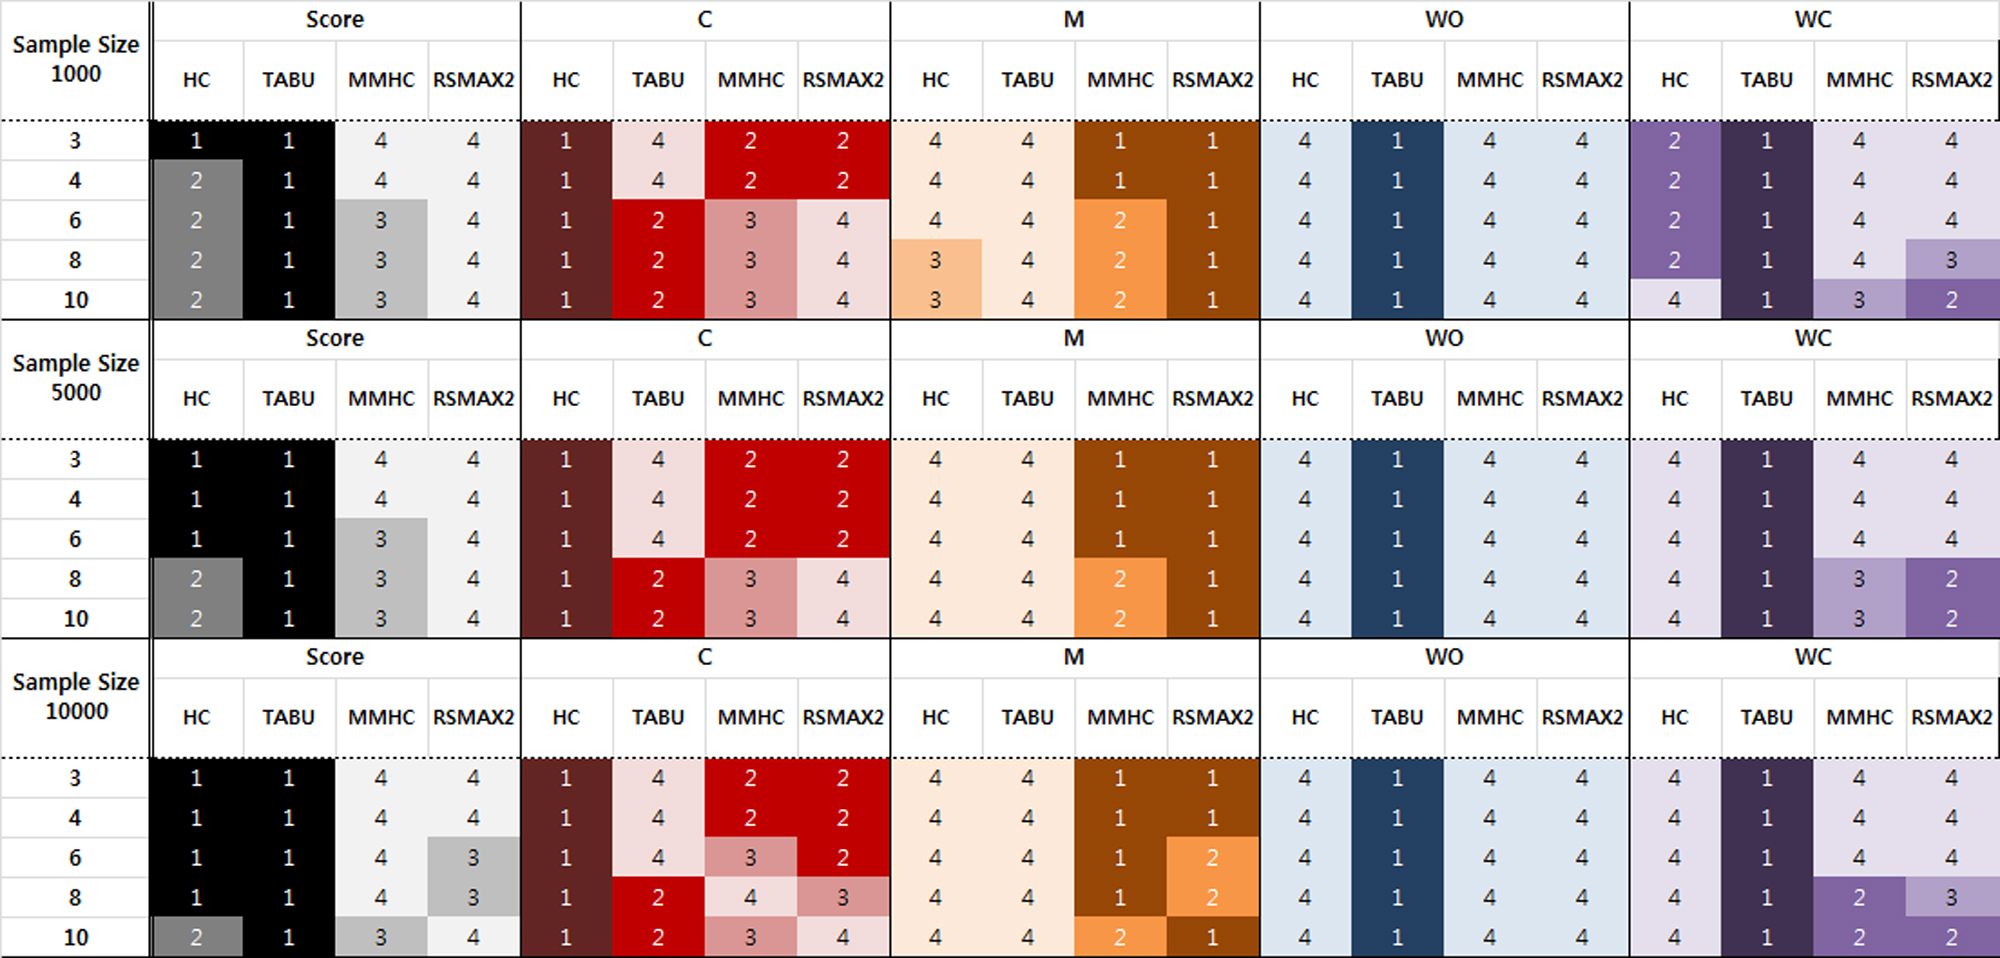
\includegraphics[height=170pt]{Result_Star}
		\caption{Summary for Comparison via Star}
	\end{figure}	

% Star 역시, 알고리즘별 성능이 크게 차이가 발생하지 않았다.
Star also, the performance of each algorithm was not different significantly occurs.

% Score 기준으로 비교했을 때는 TABU search가 좋은 성능을 보여주었지만, 목표 네트워크와 학습 네트워크를 비교했을 경우, 상대적으로 Hill-climbing이 line 형태에서 좋은 성능을 보여주었다.
Although TABU search when compared on the basis of exhibited good performance Score, when compared to the network and learning network objectives, relatively Hill-climbing showed good performance in the line form.

% 특이한 점은, node 개수가 작을 때, TABU search는 score에 따른 성능이 좋음에도 불구, 다른 알고리즘에 비해 C의 개수가 압도적으로 적고, M, WO, WC의 개수가 무척 높은 모습이 나타났다. 그러나 node 개수가 많아질수록, sample size가 커질수록 다른 알고리즘에 비해 C의 개수가 많아지고, M, WO, WC의 개수가 줄어드는 현상이 나타났다.
Specific point, when the node number is small, TABU search despite the good performance by score, the number of C is overwhelmingly smaller than the other algorithms, M, WO, very few of the WC high figure was revealed. However, as the number of node increases, becoming the number of C is increased as compared with the sample size becomes large as the other algorithms, M, WO, a phenomenon that the number decreases of WC appeared.

% 그럼에도 불구하고 Hill-climbing의 성능에 미치지는 못하였다.
And yet, did not give the performance of Hill-climbing.

% 모든 알고리즘이,Sample size가 커짐에 따라 WO, WC 개수가 크게 줄어드는 모습이 나타났다.
All algorithms, WO as Sample size increases, how the number of WC is greatly reduced revealed.
	
	\begin{figure}[p]
	\centering
		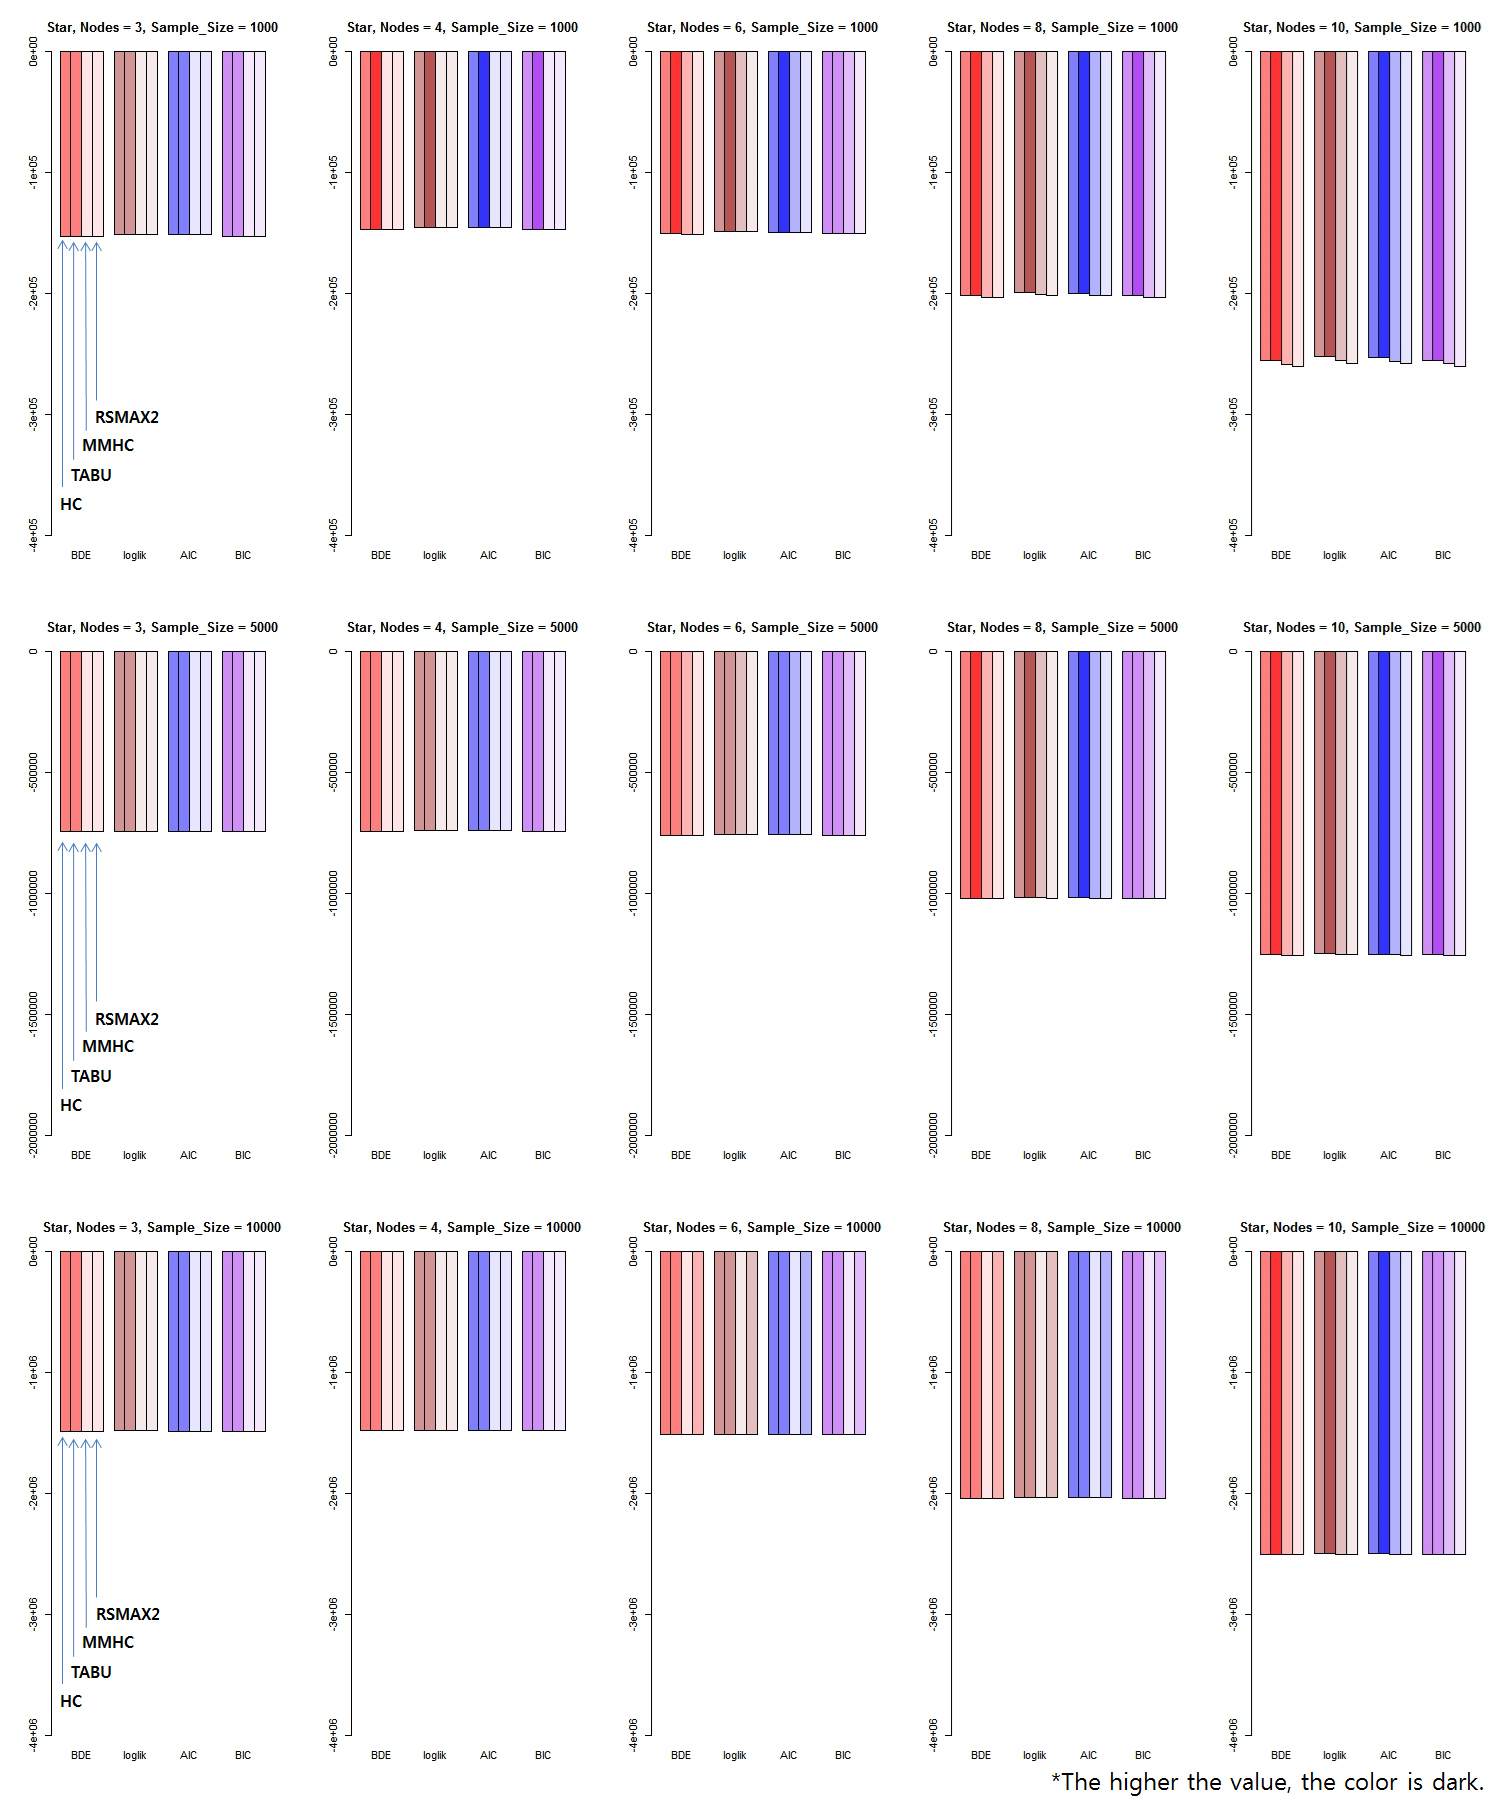
\includegraphics[height=500pt]{03_Star_Score}
		\caption{Comparison of scores via Star}
	\end{figure}	

	\begin{figure}[p]
	\centering
		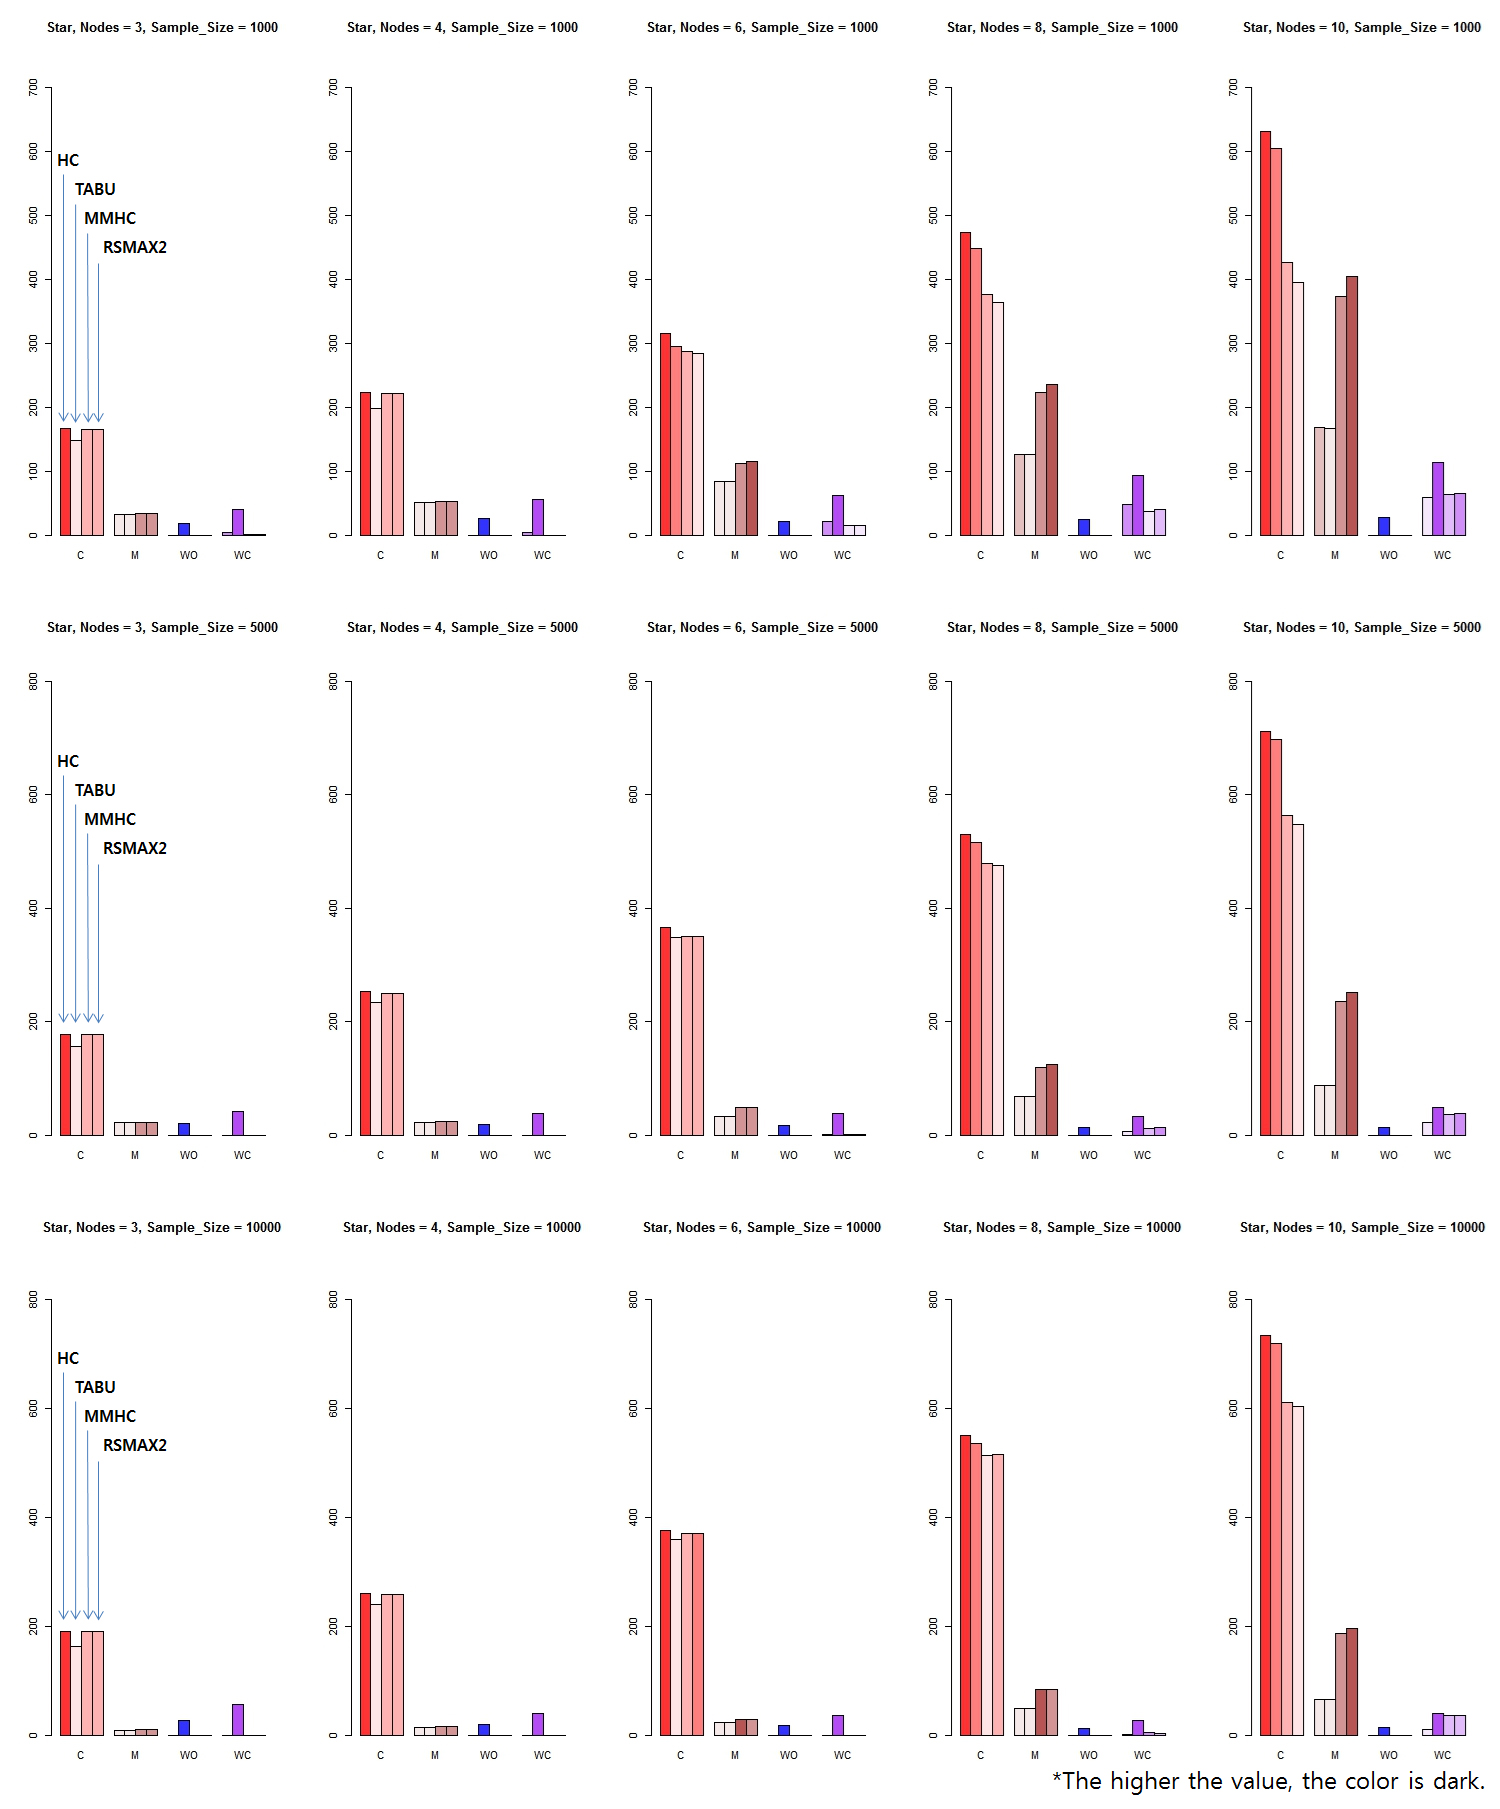
\includegraphics[height=500pt]{03_Star_Arcs}
		\caption{Comparison of correct arcs via Star}
	\end{figure}	


\newpage{}

\subsection{Pseudo Loop}
	\begin{figure}[h]
	\centering
		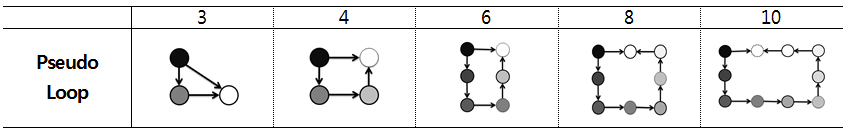
\includegraphics[height=50pt]{Topologies_PseudoLoop}
		\caption{Bayesian Network Topologies : Pseudo Loop}
	\end{figure}	

	% Pseudo Loop은, 우선 line 형태를 그린 뒤, 최상의 부모 node가 맨 마지막 자식 node에 종속되는 arc가 추가된 형태이다. 사실 loop는 아니지만, 얼핏 보면 loop처럼 보인다. (사실, 정말 loop가 만들어지면 더 이상 Bayesian Network가 아니다.)
	Pseudo Loop, after first drew a line form, is the best form of arc has been added to the parent node is dependent on the very last child node. Actually loop does not have, it looks like a loop at first glance. (In fact, actually when loop is created, no longer Bayesian Network is not it.)

\begin{figure}[!bhp]
	\centering
		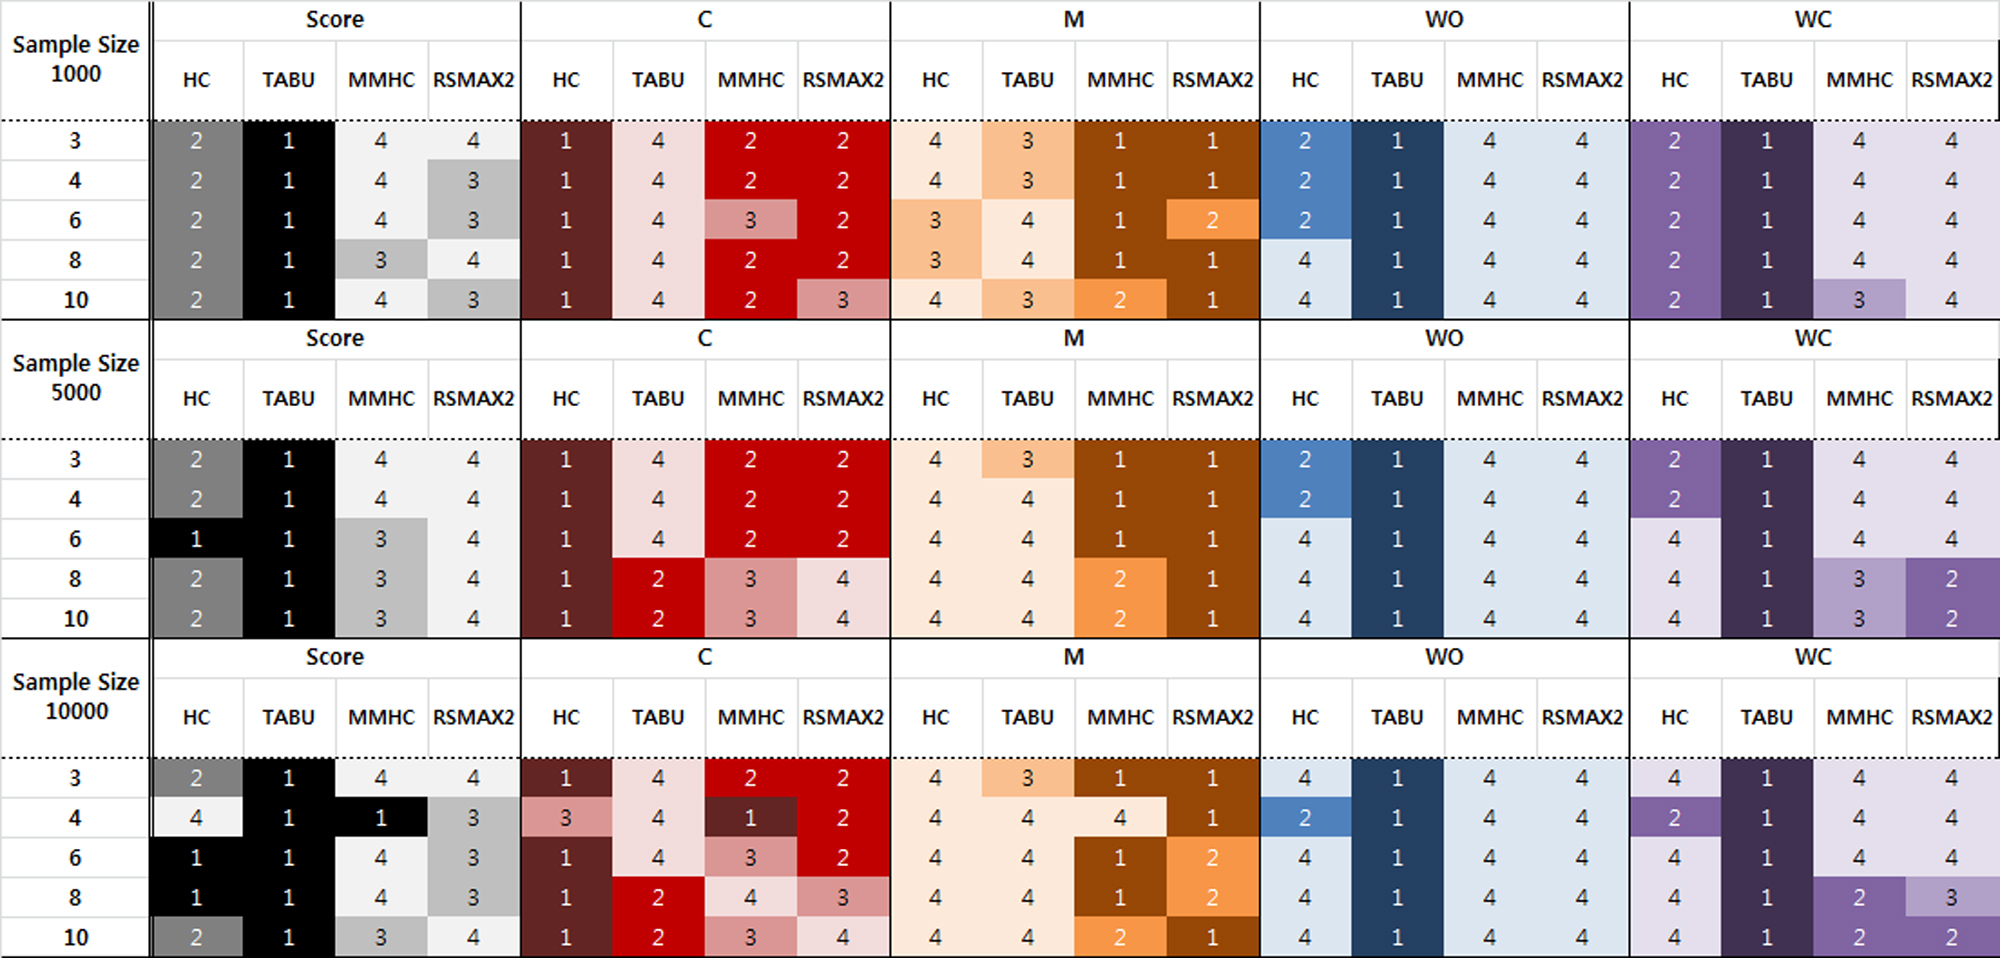
\includegraphics[height=170pt]{Result_PseudoLoop}
		\caption{Summary for Comparison via Pseudo Loop}
	\end{figure}	

% Score 기준으로 비교했을 때는 TABU search가 좋은 성능을 보여주었지만, 목표 네트워크와 학습 네트워크를 비교했을 경우, 상대적으로 Hill-climbing이 line 형태에서 좋은 성능을 보여주었다.
Although TABU search when compared on the basis of exhibited good performance Score, when compared to the network and learning network objectives, relatively Hill-climbing showed good performance in the line form.

% sample size가 1000개일 때는 TABU search의 C의 개수가 개선되지 못했지만, sample size가 커지면 node 개수가 많을 때 C의 개수가 크게 향상되는 모습을 보여주었다. 특히 sample size 증가에 따른 M, WO, WC의 개수 감소가 두드러졌다. 그럼에도 불구하고 Hill-climbing의 성능에 미치지는 못하였다.
If the sample size is 1000 exists, the number of C of TABU search has not been improved, I shows how the number of C when sample size is often node number becomes larger is greatly improved. In particular M with increasing sample size, WO, the reduction in the number of WC was noticeable. And yet, did not give the performance of Hill-climbing.

% 모든 알고리즘이,Sample size가 커짐에 따라 WO, WC 개수가 크게 줄어드는 모습이 나타났다.
All algorithms, WO as Sample size increases, how the number of WC is greatly reduced revealed.
	
	\begin{figure}[p]
	\centering
		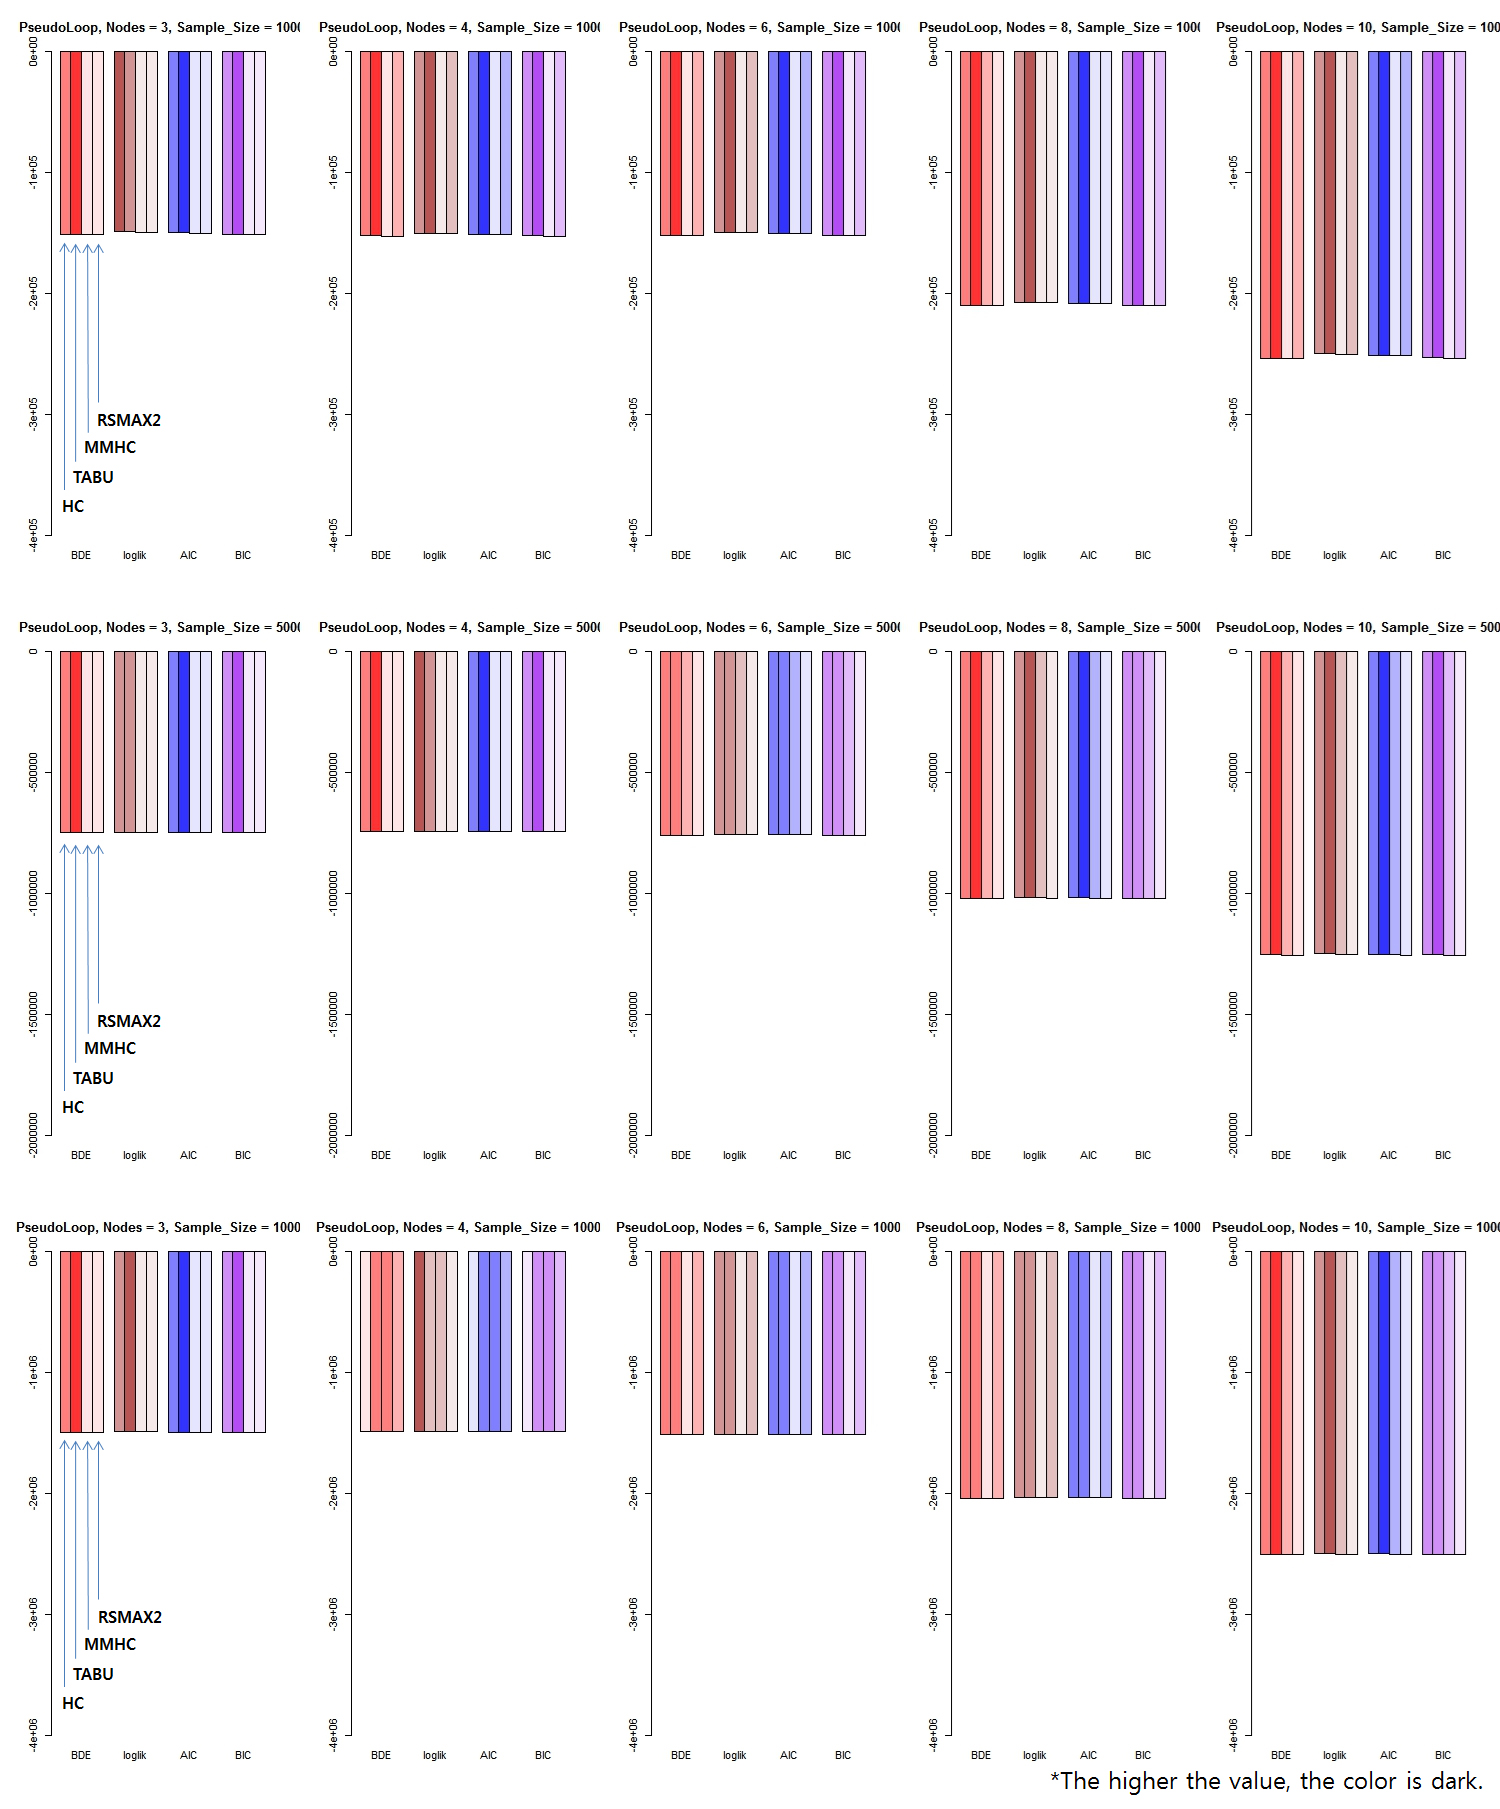
\includegraphics[height=500pt]{04_PseudoLoop_Score}
		\caption{Comparison of scores via Pseudo Loop}
	\end{figure}	

	\begin{figure}[p]
	\centering
		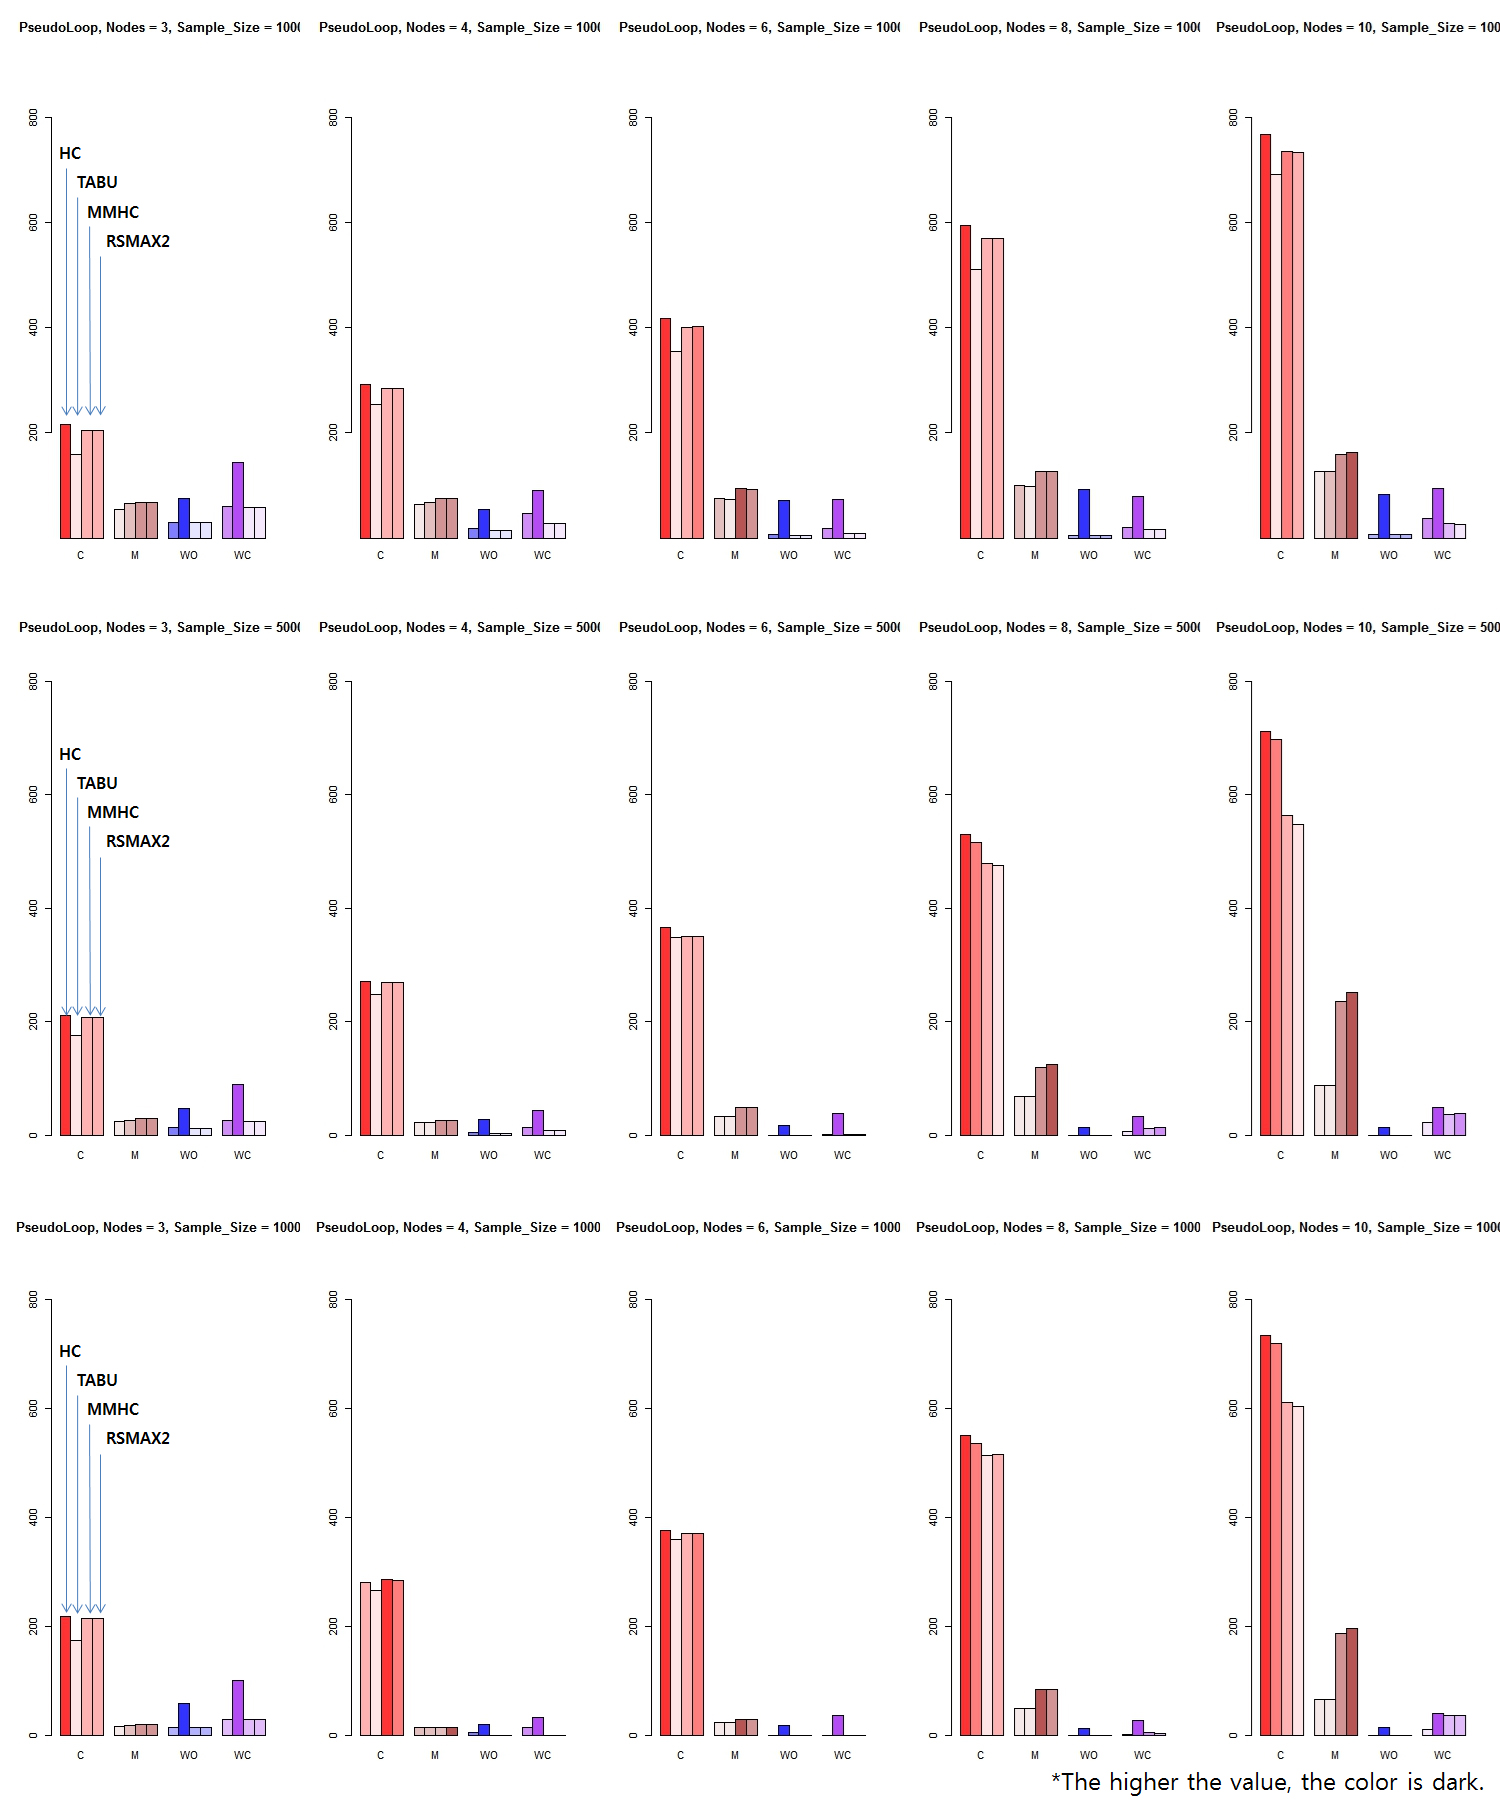
\includegraphics[height=500pt]{04_PseudoLoop_Arcs}
		\caption{Comparison of correct arcs via Pseudo Loop}
	\end{figure}	


\newpage{}

\subsection{Diamond}
	\begin{figure}[h]
	\centering
		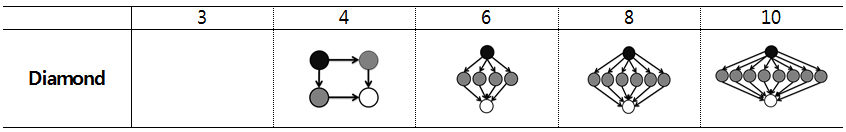
\includegraphics[height=50pt]{images/Topologies_Diamond}
		\caption{Bayesian Network Topologies : Diamond}
	\end{figure}	

	% Diamond는 윗 부분은 한 개의 node가 여러 개의 자식 node를 가진 Star 형태이고, 아래 부분은 한 개의 자식 node가 여러 개의 부모 node를 가진 Collapse 형태이다.
	A part of the top, one node has plurality of child node like Star form. And the bottom part, one node has plurality of parent node like Collapse form. If it connected, then it called Diamond.
	
\begin{figure}[!bhp]
	\centering
		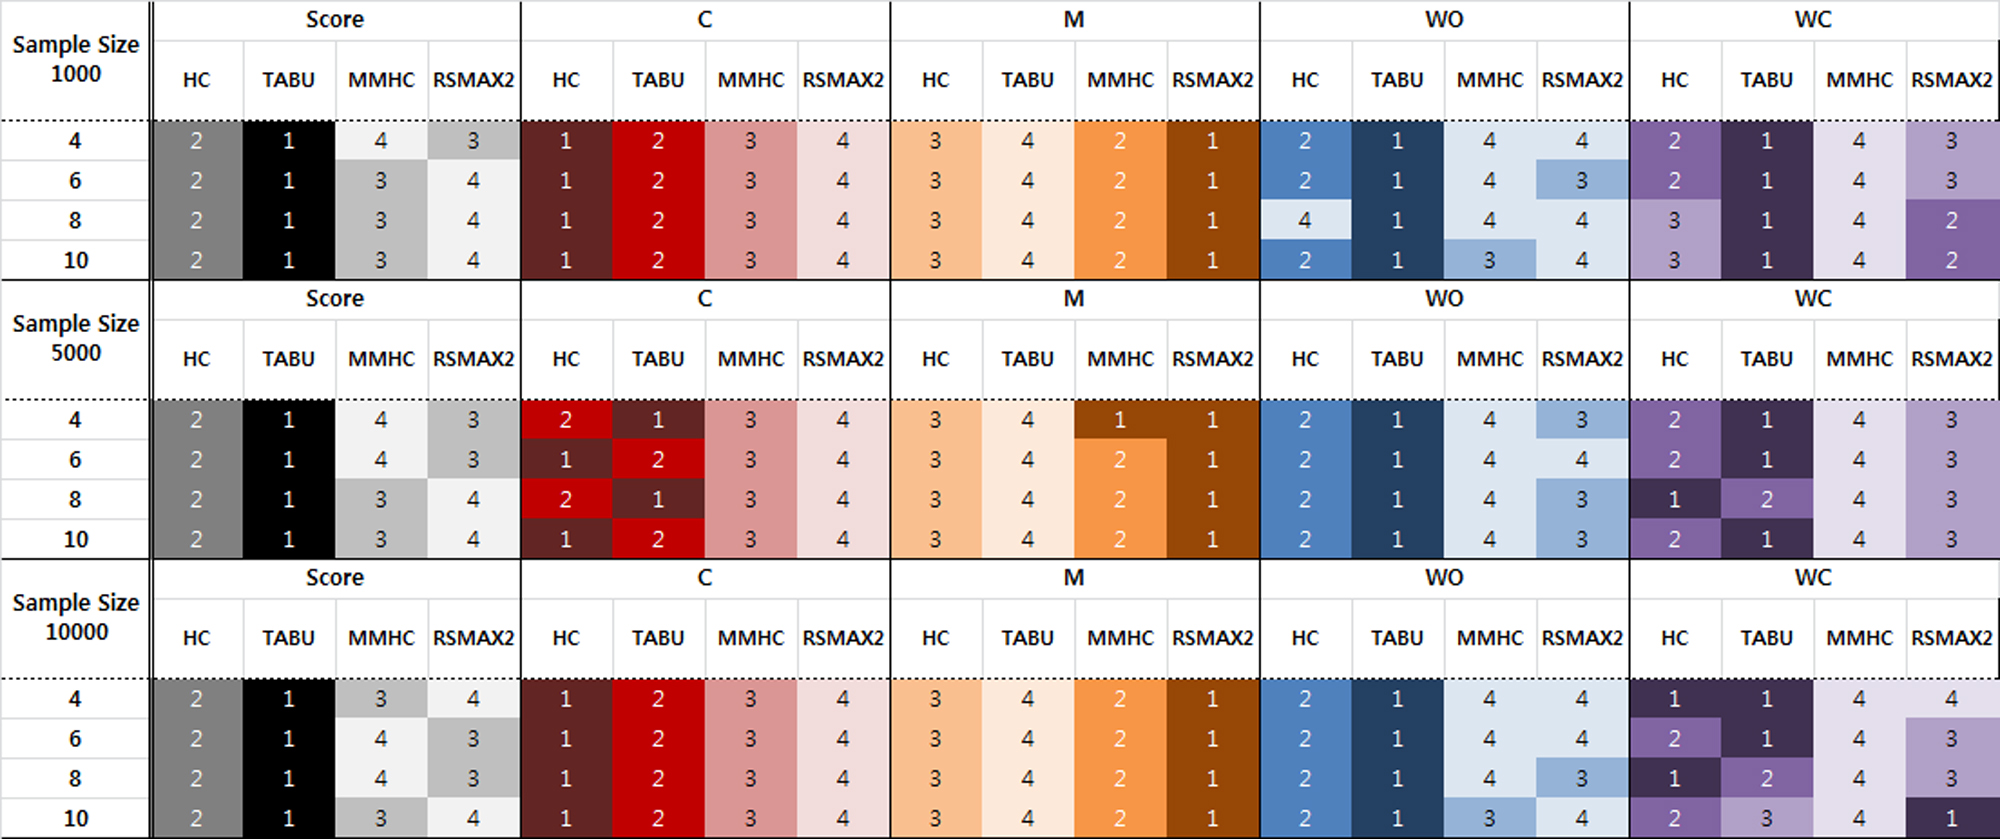
\includegraphics[height=155pt]{images/Result_Diamond}
		\caption{Summary for Comparison via Diamond}
	\end{figure}	

% Score, C 기준으로 비교했을 때 각각 TABU search, Hill-climbing이 좋은 성능을 나타냈다. 하지만 WO, WC도 많은 것으로 나타났다
Respectively, when compared to the score and C,  TABU search and Hill-climbing showed a good performance. However, WO, WC also showed that many.

% WO, WC가 적은 것을 기준으로 보았을 때 MMHC가 유리한 것으로 나타났다. RSMAX2는 WC가 많이 나타났다.
when compared to the WO and WC, MMHC showed that advantageous. RSMAX2 showed a lot of WC.

% 이러한 현상은 sample size가 커질수록, node 개수가 많아질수록 두드러졌다.
This phenomenon was stood out when the larger the sample size or the node.
	
	\begin{figure}[p]
	\centering
		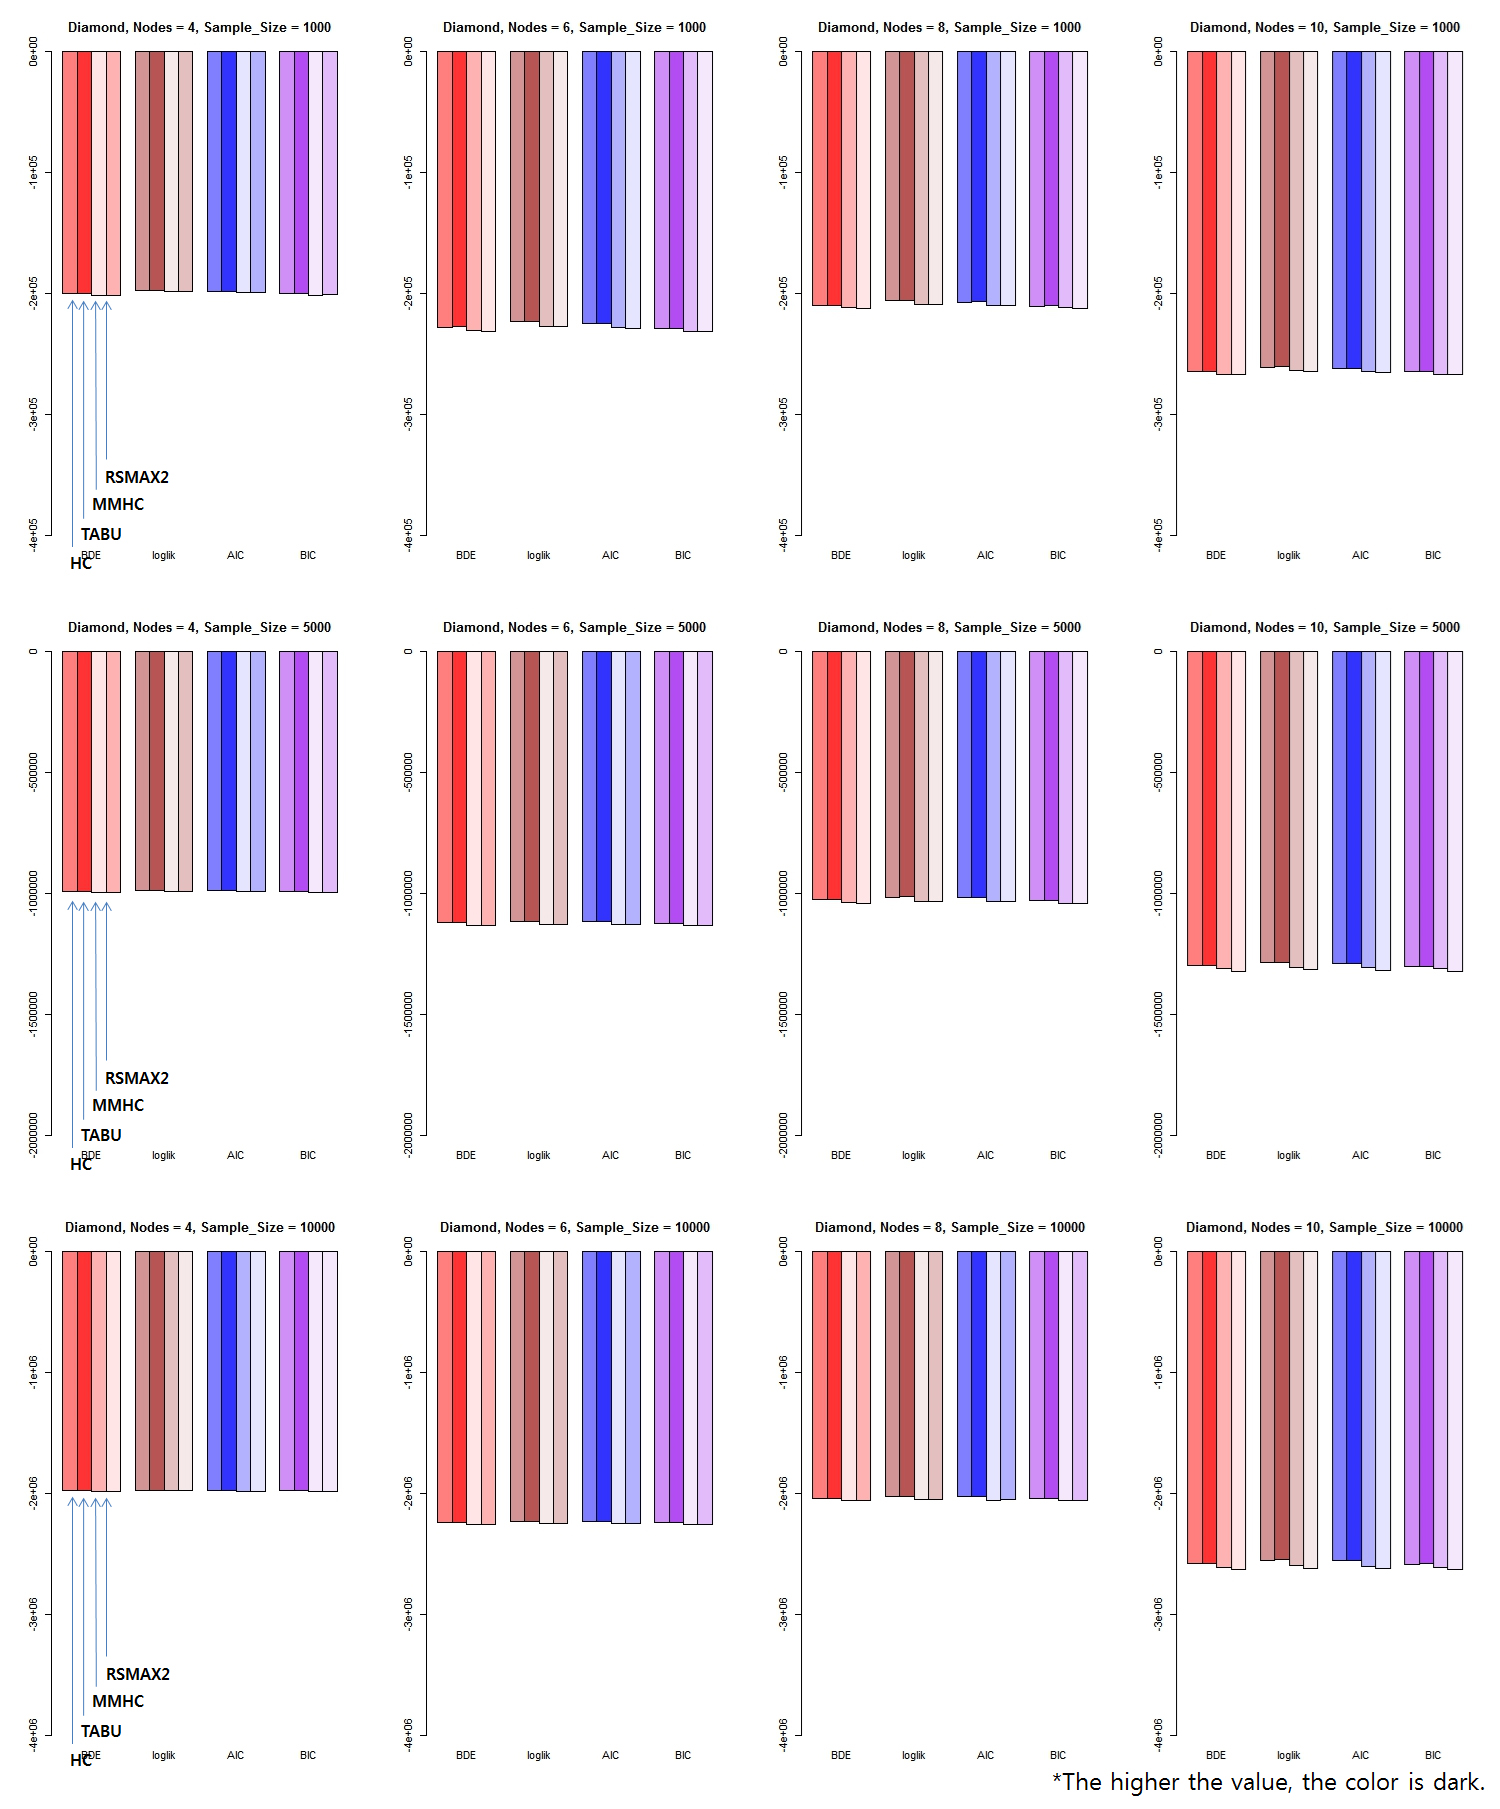
\includegraphics[height=500pt]{images/05_Diamond_Score}
		\caption{Comparison of scores via Diamond}
	\end{figure}	

	\begin{figure}[p]
	\centering
		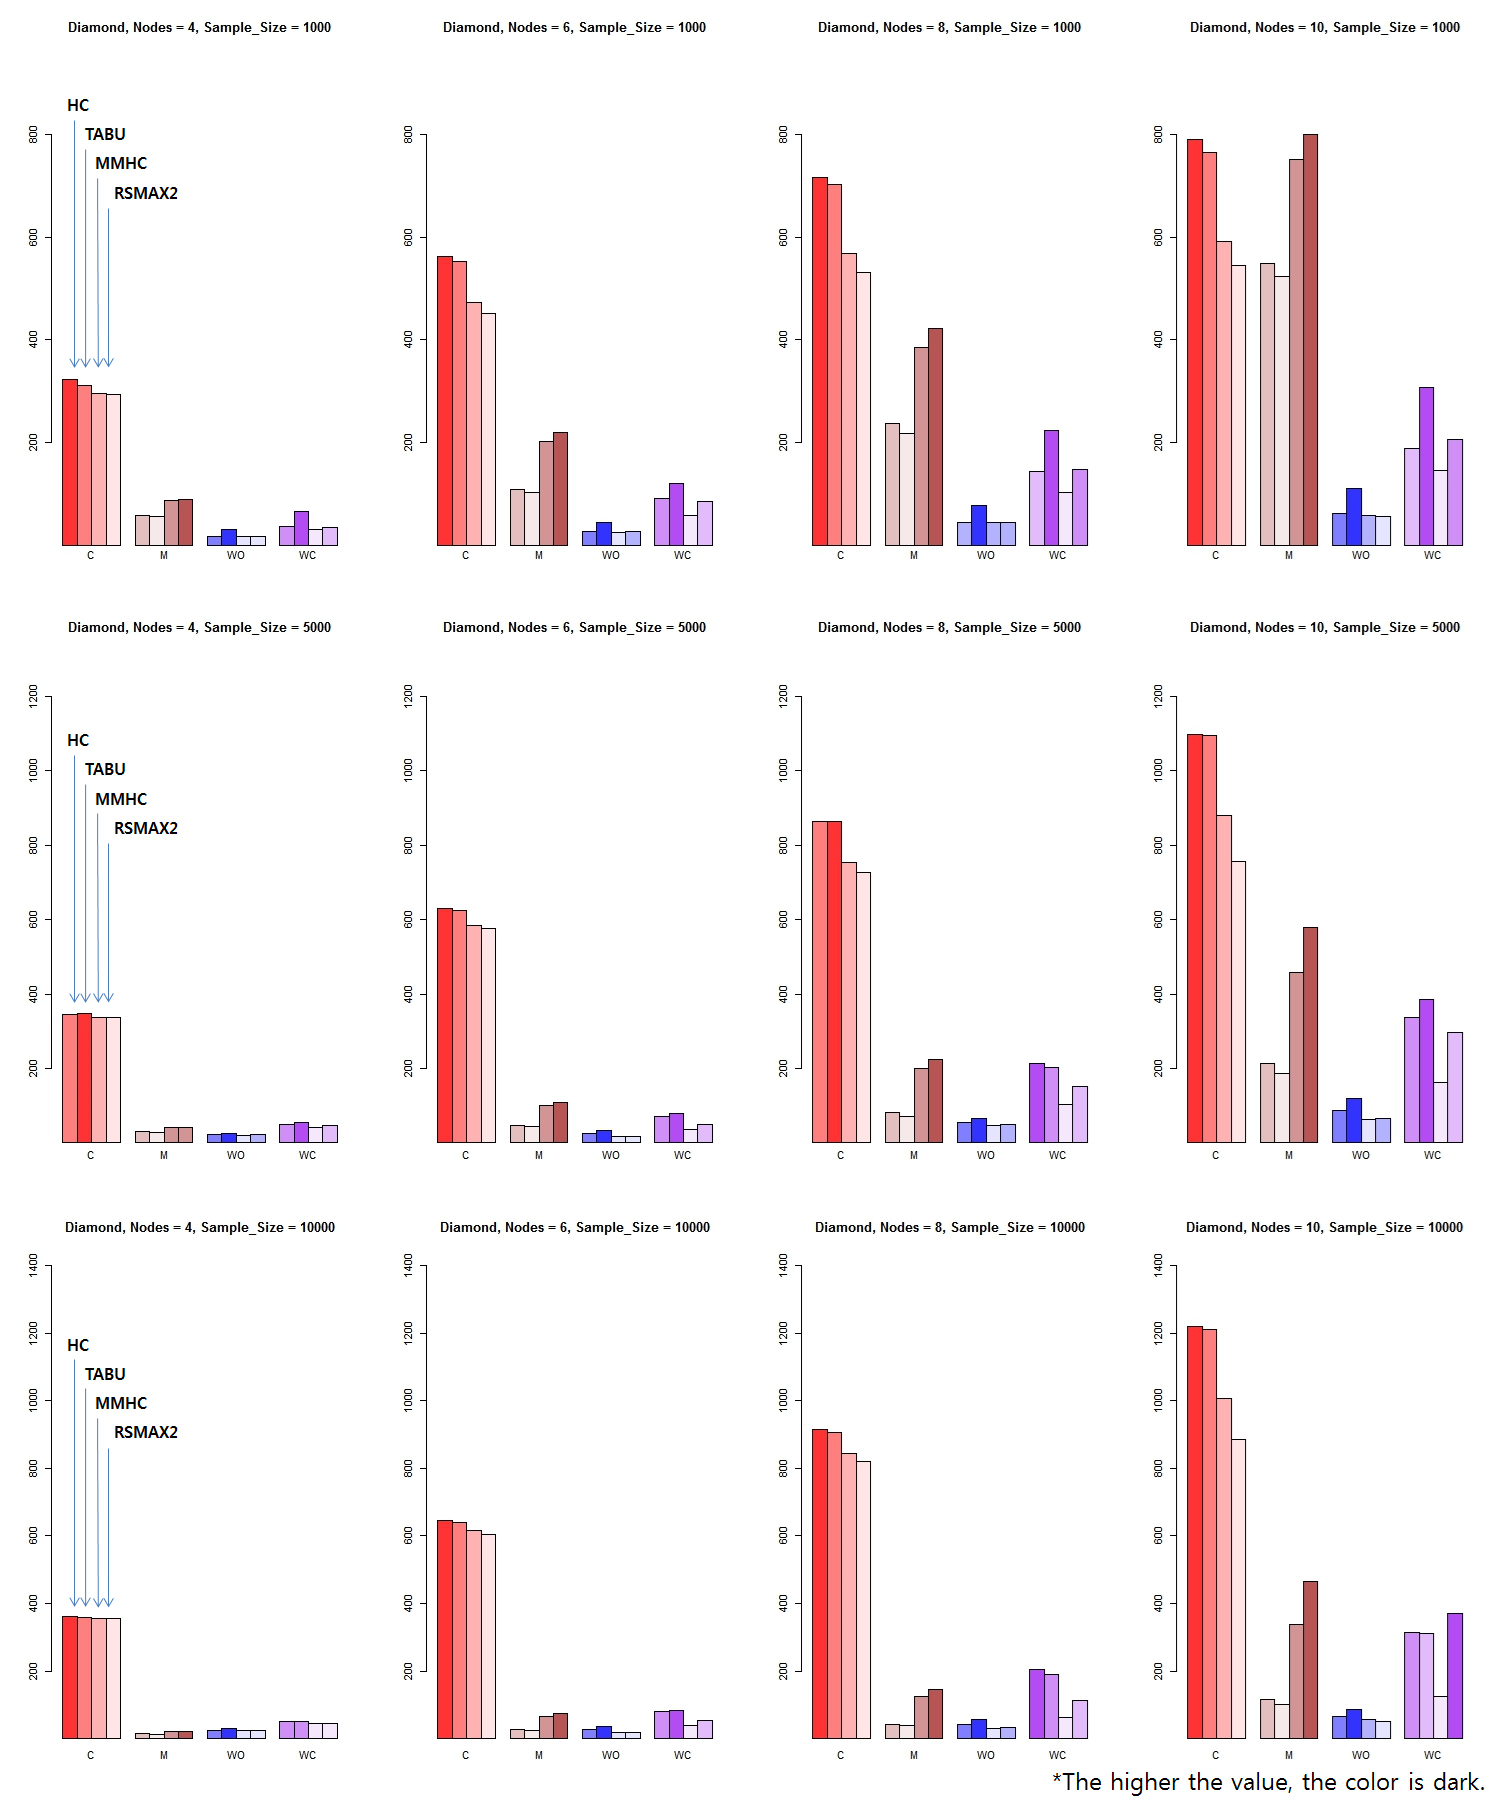
\includegraphics[height=500pt]{images/05_Diamond_Arcs}
		\caption{Comparison of correct arcs via Diamond}
	\end{figure}	
	

\newpage{}

\subsection{Rhombus}
	\begin{figure}[h]
	\centering
		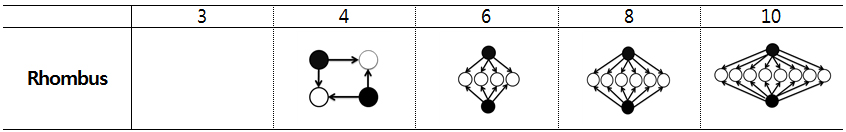
\includegraphics[height=50pt]{Topologies_Rhombus}
		\caption{Bayesian Network Topologies : Rhombus}
	\end{figure}	

	% Rhombus는 두 개의 node가 여러 개의 자식 node를 함께 가진 형태이다.
	Rhombus is in the form of two of the node is attached multiple of the child node together.

\begin{figure}[!bhp]
	\centering
		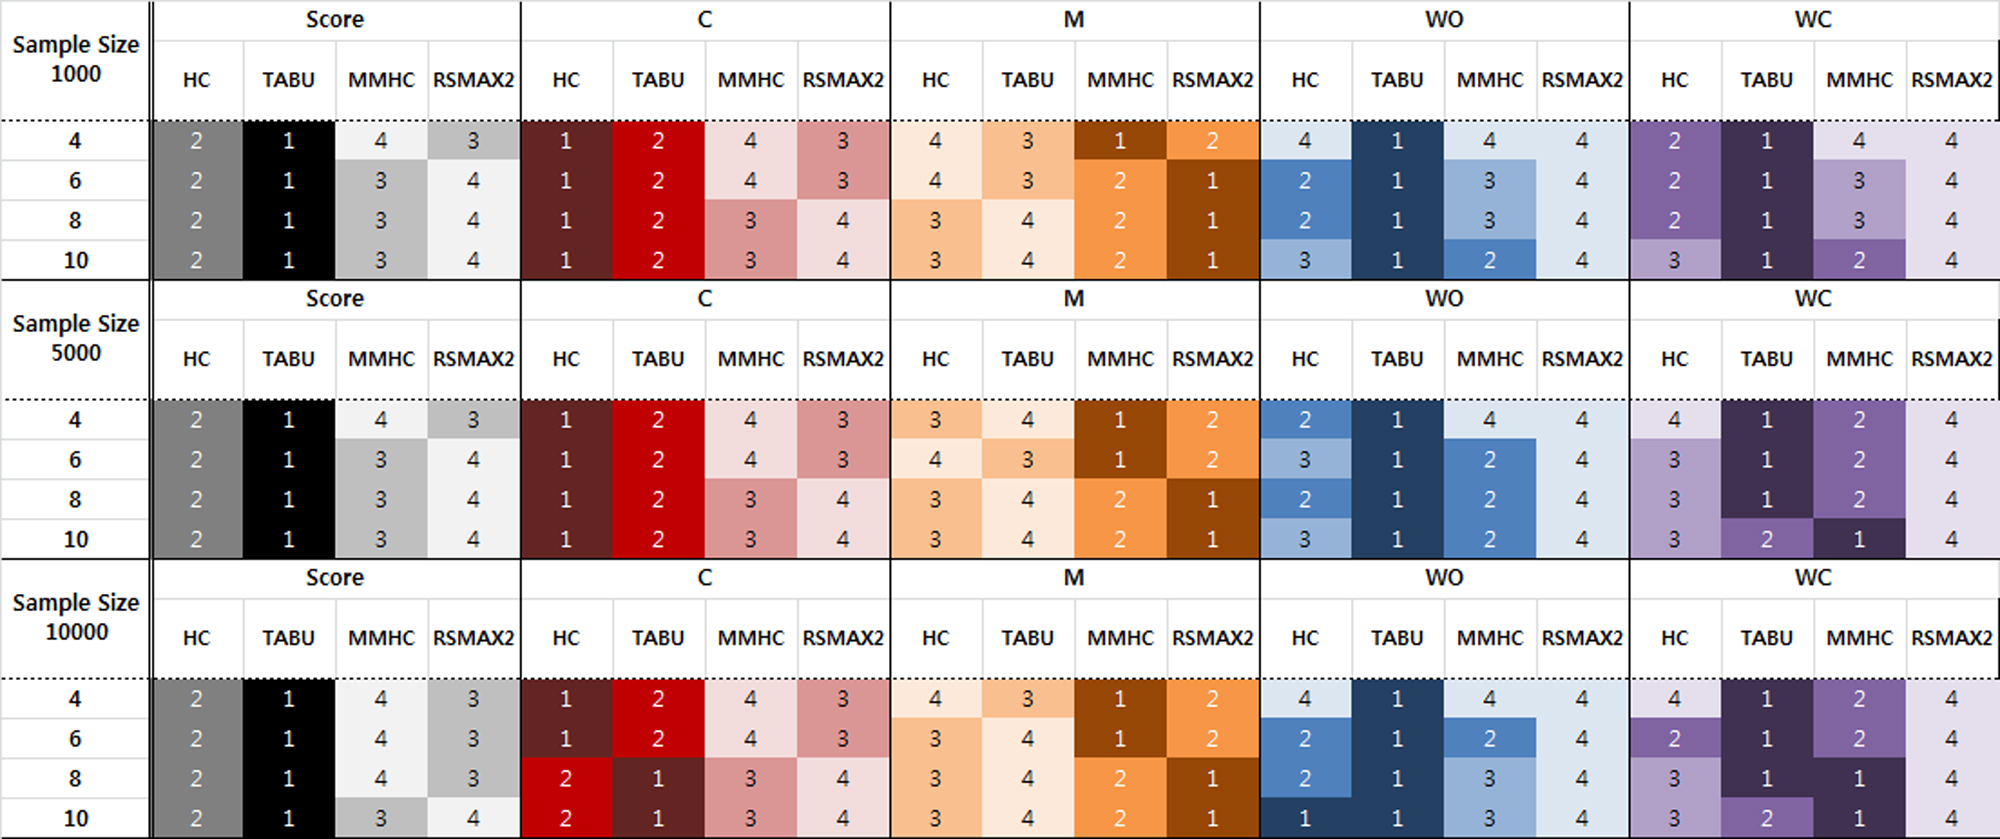
\includegraphics[height=170pt]{Result_Rhombus}
		\caption{Summary for Comparison via Rhombus}
	\end{figure}	

% Score, C 기준으로 비교했을 때 각각 TABU search, Hill-climbing이 좋은 성능을 나타냈다.
Score, when compared on the basis of the C, TABU search, the Hill-climbing showed good performance, respectively.

% 하지만 WO, WC도 많은 것으로 나타났다.
However, WO, WC was also found many things.

% WO, WC가 적은 것을 기준으로 보았을 때 RSMAX2가 유리한 것으로 나타났다. 오히려 MMHC는 WC가 많이 나타났다.
WO, RSMAX2 when viewed relative to that WC is small it was found to be advantageous. Rather MMHC became many WC.

% 다만 sample size가 커짐에 따라 모든 알고리즘의 성능이 전반적으로 개선되는 모습이 나타났다.
However as the sample size increases, how the performance of all algorithms is overall improvement was revealed.
	
	\begin{figure}[p]
	\centering
		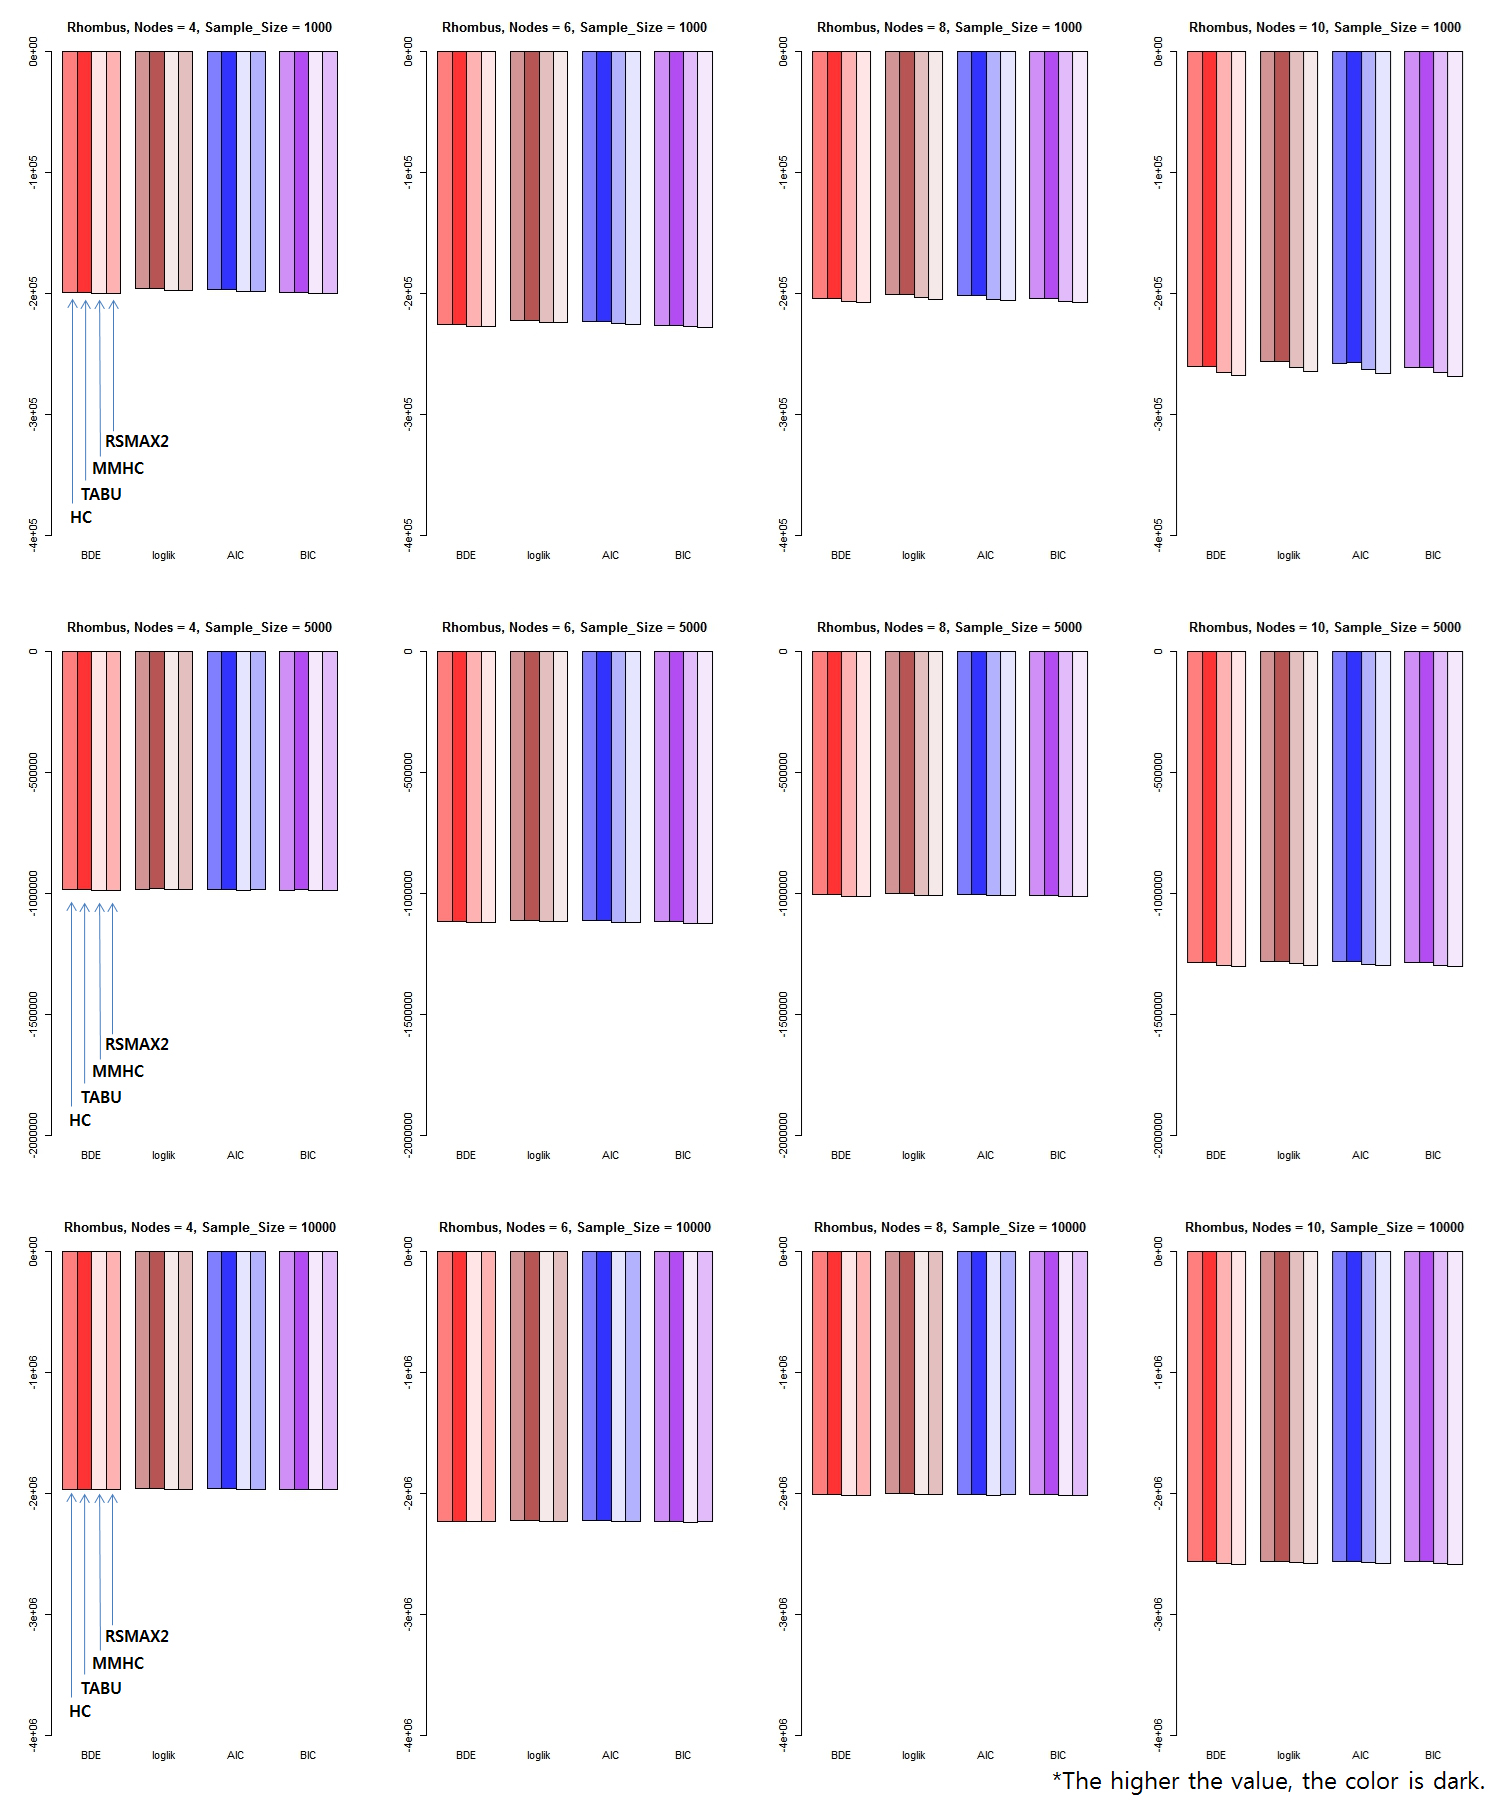
\includegraphics[height=500pt]{06_Rhombus_Score}
		\caption{Comparison of scores via Rhombus}
	\end{figure}	

	\begin{figure}[p]
	\centering
		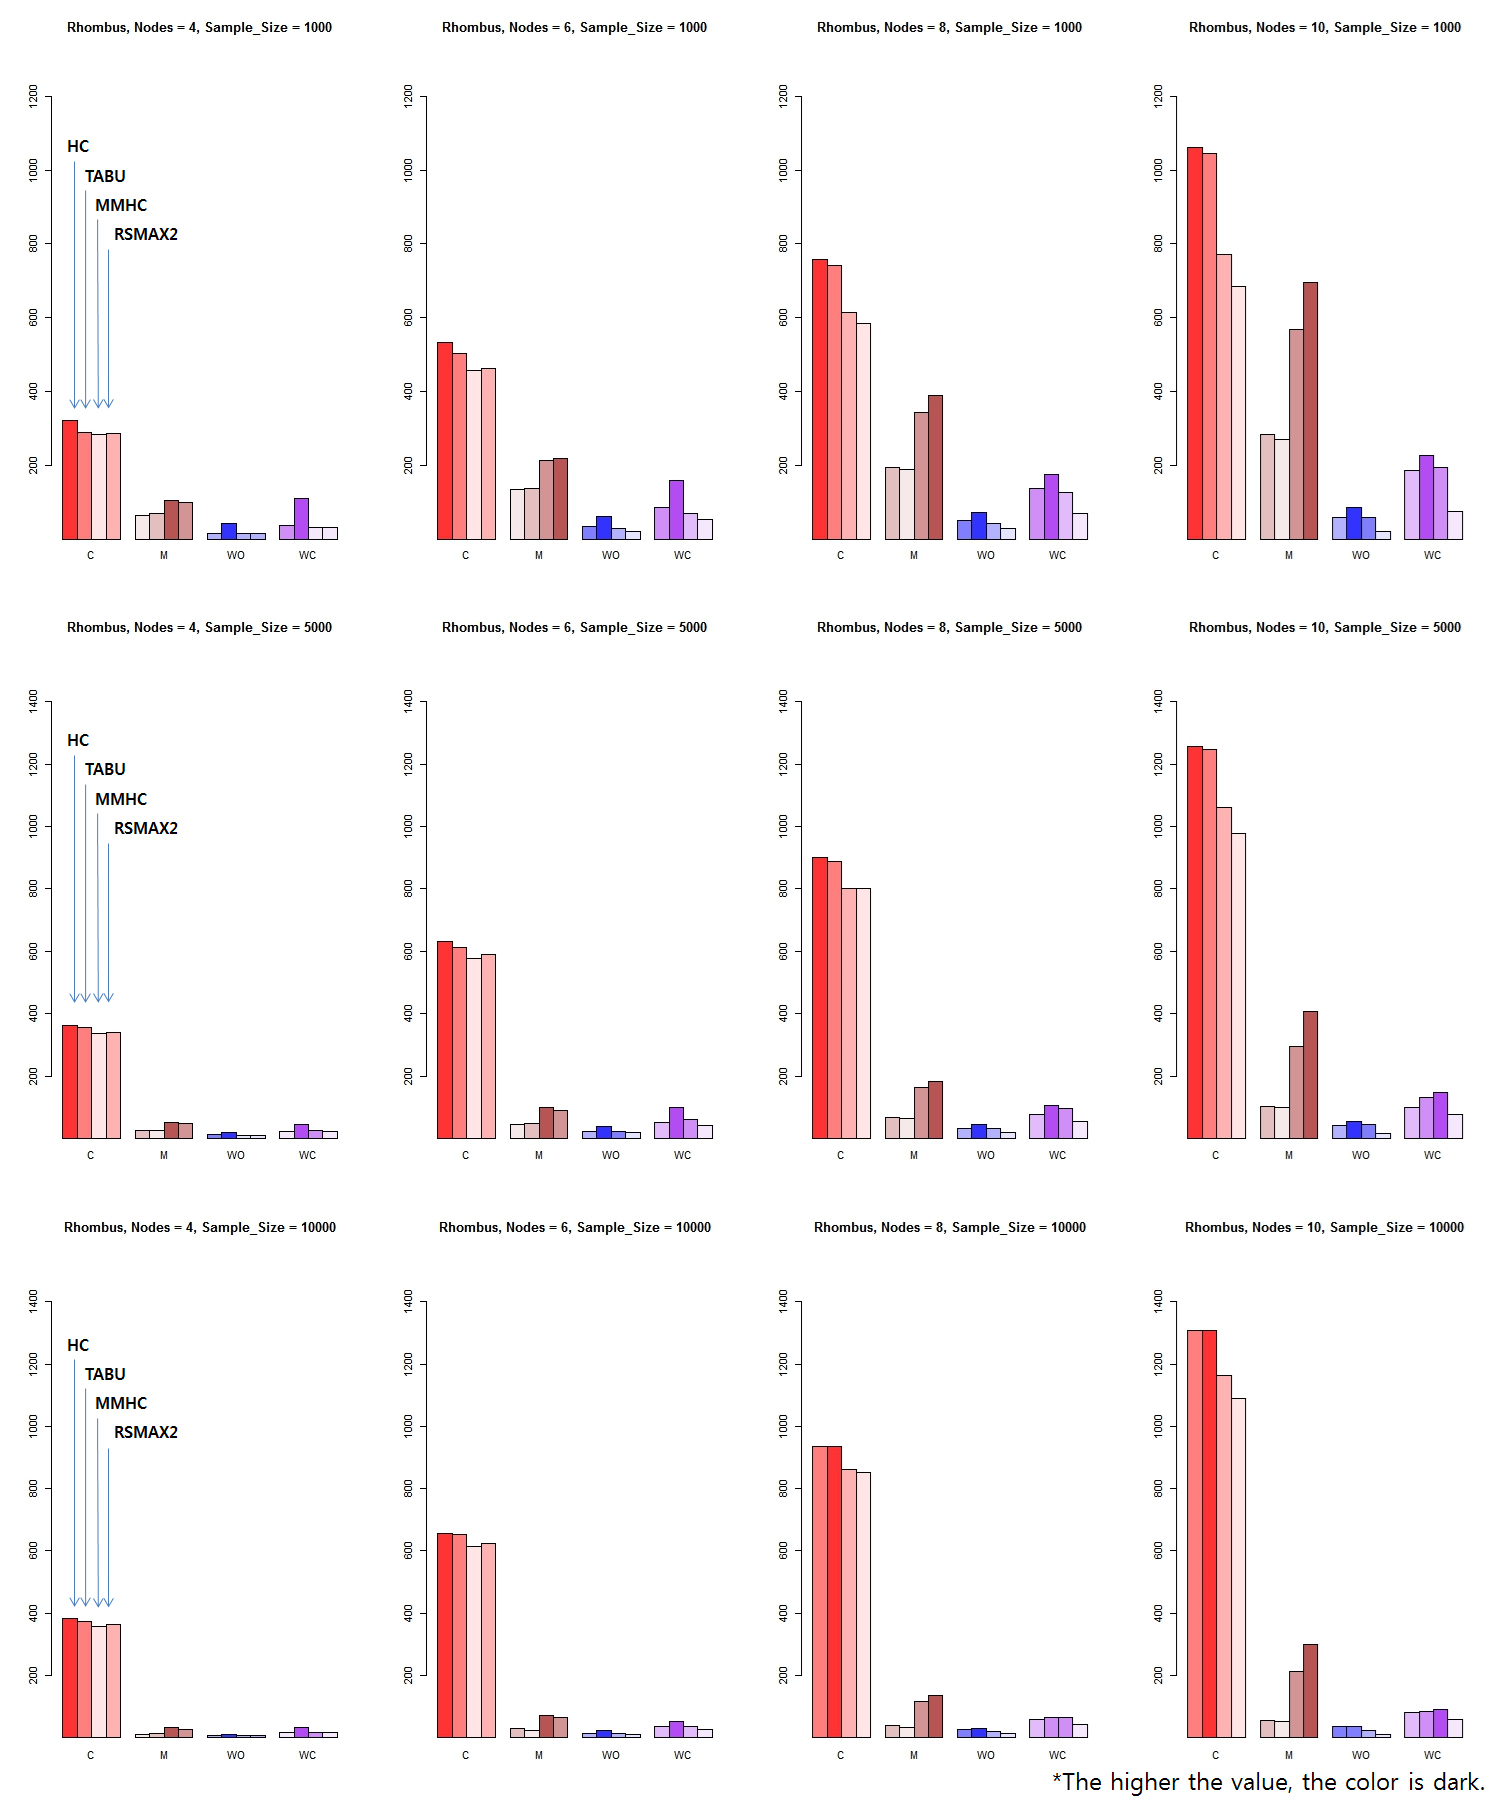
\includegraphics[height=500pt]{06_Rhombus_Arcs}
		\caption{Comparison of correct arcs via Rhombus}
	\end{figure}	






\chapter{Discussion}
% ~~~~Topology에 따른 알고리즘별 성능을 비교해본 결과, score 기준으로는 TABU search가 대부분 가장 좋은 것으로 나타났다. 하지만 목표 네트워크와 학습 네트워크를 직접 비교해본 결과 "C가 무엇이 가장 많은가"를 기준으로 하였을 때는 Hill-climbing이 성능이 좋은 것으로 나타날 때가 많았다. 오히려 TABU search는 WO와 WC가 많은 것으로 나타났다.
~~~~Result of comparing the performance of each algorithm according to the Topology, TABU search has been found most best thing by score criteria. However, as a result of comparing between the target network and learning network directly, when a reference to "What C is a lot?" is, Hill-climbing was often appears that the performance is good. Rather TABU search has a lot of WO and WC.

% Score-based 알고리즘에 비해 Hybrid 알고리즘이 arc를 더 보수적으로 그려주는 것으로 나타났다. 이에 따라 C가 적고 missing arcs가 많지만, WO, WC가 매우 적게 나타나기 때문에, WO, WC가 그려지는 것이 치명적일 경우 이 알고리즘을 사용할 수 있을 것으로 보인다. 특히 Diamond 형태에 대해서는 MMHC가, Rhombus 형테에 대해서는 RSMAX2가 유리한 것으로 보인다.
Hybrid algorithm compared to Score-based algorithm is found to be that draw the arc more conservative. This makes not only C is often less missing arcs, but also WO and WC is drawn very small. It seems to use when WO and WC are fatal. Especially MMHC for Diamond form, RSMAX2 for Rhombus seems to be advantageous.

% Line과 Star 형태는 다른 topology에 비해 상대적으로 알고리즘에 따른 성능 차이가 나지 않았다.
About Line and Star form, the performance difference due to relatively algorithm was not large compared to other topology.

% 대부분의 topology에서, node의 개수가 작을 때에는 알고리즘별 성능 차이가 나지 않았지만, node의 개수가 많아질수록 알고리즘별 성능 차이가 두드러지는 현상이 나타났다. 또, Sample size가 커질수록 M, WO, WC의 빈도가 작아지는 현상이 나타났다.
In most of the topology, when the sample size is small, the number of C has not been improved. However, sample size is larger, then C was increased. In addition, M, WO and WC was decreased.

% 이들을 바탕으로, 베이지안 네트워크 구조 학습을 진행하는 연구자는, 자신의 목표 네트워크가 어떠한 형태인가에 따라 어떠한 알고리즘을 선택할지 고려해볼 수 있을 것이다. 또한 학습 네트워크에 M, WO, WC가 많으면 치명적일 경우, Hybrid 알고리즘 선택을 고려해볼 수 있을 것이다.
On the basis of these results, algorithm users will be able to try to consider whether to choose what algorithms depending on whether their target network is any way. Especially, when the many M, WO, WC is fatal, it will be able to try to consider the selection of hybrid algorithm.

% 이 연구는 앞으로 topology의 node 개수를 증가시키거나, sample size를 더 적게 하여, 혹은 cardinality를 증가시켜 추가 실험을 할 수 있다. 또 다른 algorithm을 적용해보거나, 두 개 이상의 topology를 서로 결합하여 비교 분석할 수도 있다.
In future study, it can be to increase the number of node topology, to less sample size, or to increase the cardinality. Or by applying another algorithms, in addition it is possible to compare analyzed by combining two or more mutually topology.

% 확률 관계를 정의할 때 확률값을 U(0,1) 사이의 값에서 임의로 주었는데, 이 확률값을 "순차적"으로 준 것과의 관계를 알아볼 수도 있다.
In this paper, the probability when defining the relationship between the probability gave arbitrarily value between $U(0,1)$. But it is possible to confirm the relationship between those given this probability "sequential" in future study.

% 그렇지만 무엇보다도 Bayesian Network Data Generator의 R 패키징을 완성하여야 할 것이다.
It is desirable to complete the R package of Bayesian network data generator more than anything else.

% 이외에도 continuous data를 이용한 분석, BN을 이용한 missing value를 컨트롤할 수 있을 것이다. 이 때 Bayesian Network Data Generator를 적극적으로 활용할 수 있을 것이다.
In addition, analysis using the continuous data. Also we will be able to control the missing value of using BN. In this case it is possible to actively utilize Bayesian network data generator.


%%%%%%%%%%%%%%%%%%%%%%%%%%%%%%%%%%				
\newpage{} % for correct header (if you realy have empty page, delete this one.)

\chapter*{Appendix}
\addcontentsline{toc}{chapter}{Appendix}
\addcontentsline{toc}{section}{A.1 Table for Collapse}
\section*{A.1 Table for Collapse}
\begin{table}[h]																										
\centering	\caption{Comparison via Collapse (Num of Nodes = 3)}	\tiny																						
{\tabcolsep=0.01in																										
\begin{tabular}{cc||cc|cc|cc||cc|cc|cc|cc}																										
\hline																										
&	&	\multicolumn{14}{c}{Collapse	(Num	of	Nodes	=	3)}\tabularnewline																			
\hline																										
\multicolumn{2}{c||}{Sample	Size}	&	\multicolumn{2}{c|}{1000}	&	\multicolumn{2}{c|}{5000}	&	\multicolumn{2}{c||}{10000}	&	&	&	\multicolumn{2}{c|}{1000}	&	\multicolumn{2}{c|}{5000}	&	\multicolumn{2}{c}{10000}\tabularnewline											
\hline																										
&	&	Sum.	&	Std.Dev.	&	Sum.	&	Std.Dev.	&	Sum.	&	Std.Dev.	&	&	&	Sum.	&	Std.Dev.	&	Sum.	&	Std.Dev.	&	Sum.	&	Std.Dev.\tabularnewline
\hline																										
\hline																										
\multirow{4}{*}{BDe} & HC &	-149310 & 	277.03 & 	-739492 & 	1456.67 & 	-1493172 & 	3026.14 & 	\multirow{4}{*}{C} & HC &	164 & 	0.56 & 	178 & 	0.44 & 	193 & 	0.26\tabularnewline													
& TABU &	-149073 & 	273.72 & 	-738889 & 	1448.5 & 	-1493171 & 	3026.14 & 	& TABU &	152 & 	0.67 & 	171 & 	0.57 & 	182 & 	0.54\tabularnewline													
& MMHC &	-149516 & 	279.61 & 	-740618 & 	1469.62 & 	-1494739 & 	3034.04 & 	& MMHC &	154 & 	0.58 & 	170 & 	0.48 & 	180 & 	0.4\tabularnewline													
& RSMAX2 &	-149516 & 	279.61 & 	-740618 & 	1469.62 & 	-1494739 & 	3034.04 & 	& RSMAX2 &	154 & 	0.58 & 	170 & 	0.48 & 	180 & 	0.4\tabularnewline													
\hline																										
\multirow{4}{*}{loglik} & HC &	-147279 & 	281.43 & 	-736966 & 	1461.14 & 	-1490429 & 	3030.09 & 	\multirow{4}{*}{M} & HC &	32 & 	0.55 & 	13 & 	0.37 & 	4 & 	0.2\tabularnewline													
& TABU &	-147026 & 	277.87 & 	-736352 & 	1452.81 & 	-1490428 & 	3030.09 & 	& TABU &	36 & 	0.52 & 	14 & 	0.35 & 	8 & 	0.27\tabularnewline													
& MMHC &	-147531 & 	284.24 & 	-738143 & 	1474.42 & 	-1492072 & 	3038.37 & 	& MMHC &	42 & 	0.57 & 	21 & 	0.43 & 	17 & 	0.38\tabularnewline													
& RSMAX2 &	-147531 & 	284.24 & 	-738143 & 	1474.42 & 	-1492072 & 	3038.37 & 	& RSMAX2 &	42 & 	0.57 & 	21 & 	0.43 & 	17 & 	0.38\tabularnewline													
\hline																										
\multirow{4}{*}{AIC} & HC &	-147817 & 	281.67 & 	-737532 & 	1461.32 & 	-1491018 & 	3030.17 & 	\multirow{4}{*}{WO} & HC &	4 & 	0.2 & 	9 & 	0.29 & 	3 & 	0.17\tabularnewline													
& TABU &	-147570 & 	278.21 & 	-736921 & 	1453.04 & 	-1491017 & 	3030.17 & 	& TABU &	12 & 	0.33 & 	15 & 	0.41 & 	10 & 	0.36\tabularnewline													
& MMHC &	-148049 & 	284.4 & 	-738693 & 	1474.51 & 	-1492635 & 	3038.37 & 	& MMHC &	4 & 	0.2 & 	9 & 	0.29 & 	3 & 	0.17\tabularnewline													
& RSMAX2 &	-148049 & 	284.4 & 	-738693 & 	1474.51 & 	-1492635 & 	3038.37 & 	& RSMAX2 &	4 & 	0.2 & 	9 & 	0.29 & 	3 & 	0.17\tabularnewline													
\hline																										
\multirow{4}{*}{BIC} & HC &	-149137 & 	282.27 & 	-739376 & 	1461.93 & 	-1493141 & 	3030.43 & 	\multirow{4}{*}{WC} & HC &	12 & 	0.48 & 	18 & 	0.58 & 	6 & 	0.34\tabularnewline													
& TABU &	-148904 & 	279.05 & 	-738775 & 	1453.8 & 	-1493140 & 	3030.43 & 	& TABU &	44 & 	1.16 & 	36 & 	1 & 	28 & 	0.99\tabularnewline													
& MMHC &	-149320 & 	284.82 & 	-740485 & 	1474.84 & 	-1494664 & 	3038.36 & 	& MMHC &	12 & 	0.48 & 	18 & 	0.58 & 	6 & 	0.34\tabularnewline													
& RSMAX2 &	-149320 & 	284.82 & 	-740485 & 	1474.84 & 	-1494664 & 	3038.36 & 	& RSMAX2 &	12 & 	0.48 & 	18 & 	0.58 & 	6 & 	0.34\tabularnewline													
\hline																										
\end{tabular}																										
}																										
\end{table}																										


\begin{table}[p]																										
\centering	\caption{Comparison  via Collapse (Num of Nodes = 4)}	\tiny																						
{\tabcolsep=0.01in																										
\begin{tabular}{cc||cc|cc|cc||cc|cc|cc|cc}																										
\hline																										
&	&	\multicolumn{14}{c}{Collapse	(Num	of	Nodes	=	4)}\tabularnewline																			
\hline																										
\multicolumn{2}{c||}{Sample	Size}	&	\multicolumn{2}{c|}{1000}	&	\multicolumn{2}{c|}{5000}	&	\multicolumn{2}{c||}{10000}	&	&	&	\multicolumn{2}{c|}{1000}	&	\multicolumn{2}{c|}{5000}	&	\multicolumn{2}{c}{10000}\tabularnewline											
\hline																										
&	&	Sum.	&	Std.Dev.	&	Sum.	&	Std.Dev.	&	Sum.	&	Std.Dev.	&	&	&	Sum.	&	Std.Dev.	&	Sum.	&	Std.Dev.	&	Sum.	&	Std.Dev.\tabularnewline
\hline																										
\hline																										
\multirow{4}{*}{BDe} & HC &	-149071 & 	917.34 & 	-749900 & 	4601.22 & 	-1577564 & 	9508.45 & 	\multirow{4}{*}{C} & HC &	230 & 	0.78 & 	256 & 	0.66 & 	260 & 	0.62\tabularnewline													
& TABU &	-149032 & 	917.06 & 	-749097 & 	4595.92 & 	-1577556 & 	9508.39 & 	& TABU &	219 & 	0.92 & 	254 & 	0.72 & 	259 & 	0.68\tabularnewline													
& MMHC &	-149952 & 	924.62 & 	-751640 & 	4613.92 & 	-1582394 & 	9544.08 & 	& MMHC &	198 & 	0.84 & 	240 & 	0.74 & 	242 & 	0.7\tabularnewline													
& RSMAX2 &	-149735 & 	923.06 & 	-751640 & 	4613.92 & 	-1582394 & 	9544.08 & 	& RSMAX2 &	204 & 	0.83 & 	240 & 	0.74 & 	242 & 	0.7\tabularnewline													
\hline																										
\multirow{4}{*}{loglik} & HC &	-146796 & 	905.56 & 	-746922 & 	4585.58 & 	-1574342 & 	9490.79 & 	\multirow{4}{*}{M} & HC &	39 & 	0.65 & 	13 & 	0.39 & 	8 & 	0.34\tabularnewline													
& TABU &	-146749 & 	905.21 & 	-746106 & 	4580.17 & 	-1574344 & 	9490.81 & 	& TABU &	38 & 	0.58 & 	11 & 	0.31 & 	8 & 	0.34\tabularnewline													
& MMHC &	-147865 & 	914.28 & 	-748779 & 	4599.09 & 	-1579382 & 	9527.98 & 	& MMHC &	69 & 	0.73 & 	28 & 	0.51 & 	27 & 	0.55\tabularnewline													
& RSMAX2 &	-147612 & 	912.5 & 	-748779 & 	4599.09 & 	-1579382 & 	9527.98 & 	& RSMAX2 &	65 & 	0.72 & 	28 & 	0.51 & 	27 & 	0.55\tabularnewline													
\hline																										
\multirow{4}{*}{AIC} & HC &	-147508 & 	909.68 & 	-747706 & 	4589.96 & 	-1575139 & 	9495.35 & 	\multirow{4}{*}{WO} & HC &	6 & 	0.24 & 	6 & 	0.24 & 	7 & 	0.29\tabularnewline													
& TABU &	-147464 & 	909.37 & 	-746895 & 	4584.59 & 	-1575138 & 	9495.35 & 	& TABU &	18 & 	0.39 & 	10 & 	0.3 & 	8 & 	0.37\tabularnewline													
& MMHC &	-148493 & 	917.79 & 	-749518 & 	4603.18 & 	-1580114 & 	9532.07 & 	& MMHC &	8 & 	0.27 & 	7 & 	0.26 & 	6 & 	0.28\tabularnewline													
& RSMAX2 &	-148254 & 	916.09 & 	-749518 & 	4603.18 & 	-1580114 & 	9532.07 & 	& RSMAX2 &	6 & 	0.24 & 	7 & 	0.26 & 	6 & 	0.28\tabularnewline													
\hline																										
\multirow{4}{*}{BIC} & HC &	-149255 & 	919.82 & 	-750261 & 	4604.23 & 	-1578012 & 	9511.79 & 	\multirow{4}{*}{WC} & HC &	20 & 	0.67 & 	14 & 	0.59 & 	18 & 	0.81\tabularnewline													
& TABU &	-149218 & 	919.58 & 	-749466 & 	4599 & 	-1578001 & 	9511.7 & 	& TABU &	60 & 	1.26 & 	28 & 	0.9 & 	16 & 	0.73\tabularnewline													
& MMHC &	-150034 & 	926.42 & 	-751926 & 	4616.5 & 	-1582753 & 	9546.82 & 	& MMHC &	24 & 	0.71 & 	14 & 	0.51 & 	12 & 	0.56\tabularnewline													
& RSMAX2 &	-149830 & 	924.93 & 	-751926 & 	4616.5 & 	-1582753 & 	9546.82 & 	& RSMAX2 &	20 & 	0.67 & 	14 & 	0.51 & 	12 & 	0.56\tabularnewline													
\hline																										
\end{tabular}																										
}																										
\end{table}																										


\begin{table}[p]																										
\centering	\caption{Comparison  via Collapse (Num of Nodes = 6)}	\tiny																						
{\tabcolsep=0.01in																										
\begin{tabular}{cc||cc|cc|cc||cc|cc|cc|cc}																										
\hline																										
&	&	\multicolumn{14}{c}{Collapse	(Num	of	Nodes	=	6)}\tabularnewline																			
\hline																										
\multicolumn{2}{c||}{Sample	Size}	&	\multicolumn{2}{c|}{1000}	&	\multicolumn{2}{c|}{5000}	&	\multicolumn{2}{c||}{10000}	&	&	&	\multicolumn{2}{c|}{1000}	&	\multicolumn{2}{c|}{5000}	&	\multicolumn{2}{c}{10000}\tabularnewline											
\hline																										
&	&	Sum.	&	Std.Dev.	&	Sum.	&	Std.Dev.	&	Sum.	&	Std.Dev.	&	&	&	Sum.	&	Std.Dev.	&	Sum.	&	Std.Dev.	&	Sum.	&	Std.Dev.\tabularnewline
\hline																										
\hline																										
\multirow{4}{*}{BDe} & HC &	-155997 & 	1596.19 & 	-764954 & 	7828.59 & 	-1544669 & 	15723.4 & 	\multirow{4}{*}{C} & HC &	284 & 	0.97 & 	371 & 	1.04 & 	384 & 	1.1\tabularnewline													
& TABU &	-155793 & 	1593.85 & 	-764558 & 	7823 & 	-1544669 & 	15723.4 & 	& TABU &	284 & 	0.99 & 	372 & 	1.01 & 	384 & 	1.1\tabularnewline													
& MMHC &	-157648 & 	1613.35 & 	-772886 & 	7916.61 & 	-1555104 & 	15832.76 & 	& MMHC &	225 & 	0.88 & 	327 & 	0.98 & 	337 & 	1.08\tabularnewline													
& RSMAX2 &	-157613 & 	1612.99 & 	-772786 & 	7916.76 & 	-1555105 & 	15832.78 & 	& RSMAX2 &	229 & 	0.88 & 	328 & 	0.99 & 	337 & 	1.08\tabularnewline													
\hline																										
\multirow{4}{*}{loglik} & HC &	-153357 & 	1570.64 & 	-759643 & 	7774.48 & 	-1538497 & 	15660.96 & 	\multirow{4}{*}{M} & HC &	88 & 	1 & 	18 & 	0.5 & 	9 & 	0.35\tabularnewline													
& TABU &	-153059 & 	1567.21 & 	-759326 & 	7769.87 & 	-1538497 & 	15660.96 & 	& TABU &	78 & 	0.92 & 	13 & 	0.37 & 	9 & 	0.35\tabularnewline													
& MMHC &	-155647 & 	1594.77 & 	-768924 & 	7878.02 & 	-1550300 & 	15784.66 & 	& MMHC &	144 & 	1.2 & 	63 & 	0.85 & 	56 & 	0.7\tabularnewline													
& RSMAX2 &	-155594 & 	1594.24 & 	-768820 & 	7878.3 & 	-1550304 & 	15784.72 & 	& RSMAX2 &	141 & 	1.21 & 	61 & 	0.84 & 	56 & 	0.7\tabularnewline													
\hline																										
\multirow{4}{*}{AIC} & HC &	-154234 & 	1579.42 & 	-761260 & 	7791.09 & 	-1540234 & 	15678.54 & 	\multirow{4}{*}{WO} & HC &	28 & 	0.55 & 	11 & 	0.31 & 	7 & 	0.29\tabularnewline													
& TABU &	-153974 & 	1576.44 & 	-760910 & 	7786.08 & 	-1540234 & 	15678.54 & 	& TABU &	38 & 	0.56 & 	15 & 	0.39 & 	7 & 	0.29\tabularnewline													
& MMHC &	-156234 & 	1600.46 & 	-770049 & 	7889.11 & 	-1551579 & 	15797.54 & 	& MMHC &	31 & 	0.56 & 	10 & 	0.3 & 	7 & 	0.33\tabularnewline													
& RSMAX2 &	-156189 & 	1600.01 & 	-769950 & 	7889.37 & 	-1551582 & 	15797.59 & 	& RSMAX2 &	30 & 	0.56 & 	11 & 	0.31 & 	7 & 	0.33\tabularnewline													
\hline																										
\multirow{4}{*}{BIC} & HC &	-156386 & 	1601.03 & 	-766529 & 	7845.25 & 	-1546496 & 	15741.92 & 	\multirow{4}{*}{WC} & HC &	88 & 	1.74 & 	42 & 	1.56 & 	24 & 	0.95\tabularnewline													
& TABU &	-156219 & 	1599.16 & 	-766072 & 	7838.94 & 	-1546496 & 	15741.92 & 	& TABU &	136 & 	2.16 & 	54 & 	1.53 & 	24 & 	0.95\tabularnewline													
& MMHC &	-157675 & 	1614.46 & 	-773714 & 	7925.28 & 	-1556190 & 	15843.99 & 	& MMHC &	72 & 	1.19 & 	24 & 	0.77 & 	16 & 	0.68\tabularnewline													
& RSMAX2 &	-157649 & 	1614.2 & 	-773632 & 	7925.46 & 	-1556190 & 	15844 & 	& RSMAX2 &	70 & 	1.18 & 	22 & 	0.63 & 	14 & 	0.65\tabularnewline													
\hline																										
\end{tabular}																										
}																										
\end{table}																										


\begin{table}[p]																										
\centering	\caption{Comparison  via Collapse (Num of Nodes = 8)}	\tiny																						
{\tabcolsep=0.01in																										
\begin{tabular}{cc||cc|cc|cc||cc|cc|cc|cc}																										
\hline																										
&	&	\multicolumn{14}{c}{Collapse	(Num	of	Nodes	=	8)}\tabularnewline																			
\hline																										
\multicolumn{2}{c||}{Sample	Size}	&	\multicolumn{2}{c|}{1000}	&	\multicolumn{2}{c|}{5000}	&	\multicolumn{2}{c||}{10000}	&	&	&	\multicolumn{2}{c|}{1000}	&	\multicolumn{2}{c|}{5000}	&	\multicolumn{2}{c}{10000}\tabularnewline											
\hline																										
&	&	Sum.	&	Std.Dev.	&	Sum.	&	Std.Dev.	&	Sum.	&	Std.Dev.	&	&	&	Sum.	&	Std.Dev.	&	Sum.	&	Std.Dev.	&	Sum.	&	Std.Dev.\tabularnewline
\hline																										
\hline																										
\multirow{4}{*}{BDe} & HC &	-207806 & 	2118.77 & 	-1014209 & 	10346.61 & 	-2008048 & 	20599.86 & 	\multirow{4}{*}{C} & HC &	309 & 	1.2 & 	514 & 	1.05 & 	557 & 	0.92\tabularnewline													
& TABU &	-207509 & 	2115.9 & 	-1014025 & 	10345.07 & 	-2007946 & 	20598.88 & 	& TABU &	316 & 	1.15 & 	516 & 	0.98 & 	556 & 	0.92\tabularnewline													
& MMHC &	-209178 & 	2132.1 & 	-1029358 & 	10508.2 & 	-2032117 & 	20868.83 & 	& MMHC &	209 & 	1.02 & 	396 & 	1.15 & 	464 & 	1.03\tabularnewline													
& RSMAX2 &	-209194 & 	2132.26 & 	-1029043 & 	10506.55 & 	-2032628 & 	20875.32 & 	& RSMAX2 &	209 & 	1.03 & 	399 & 	1.18 & 	463 & 	1.04\tabularnewline													
\hline																										
\multirow{4}{*}{loglik} & HC &	-204583 & 	2088.08 & 	-1002152 & 	10217.44 & 	-1991302 & 	20420.06 & 	\multirow{4}{*}{M} & HC &	229 & 	1.49 & 	55 & 	0.73 & 	26 & 	0.48\tabularnewline													
& TABU &	-204078 & 	2083.15 & 	-1001816 & 	10214.49 & 	-1991074 & 	20417.87 & 	& TABU &	198 & 	1.36 & 	39 & 	0.58 & 	23 & 	0.47\tabularnewline													
& MMHC &	-206772 & 	2109.57 & 	-1023648 & 	10452.84 & 	-2022890 & 	20778.21 & 	& MMHC &	326 & 	1.54 & 	175 & 	1.32 & 	120 & 	0.97\tabularnewline													
& RSMAX2 &	-206802 & 	2109.89 & 	-1023214 & 	10450.49 & 	-2023458 & 	20785.37 & 	& RSMAX2 &	325 & 	1.59 & 	170 & 	1.33 & 	121 & 	1\tabularnewline													
\hline																										
\multirow{4}{*}{AIC} & HC &	-205579 & 	2097.77 & 	-1005799 & 	10256.47 & 	-1996126 & 	20471.38 & 	\multirow{4}{*}{WO} & HC &	62 & 	0.75 & 	31 & 	0.6 & 	17 & 	0.4\tabularnewline													
& TABU &	-205163 & 	2093.71 & 	-1005524 & 	10254.08 & 	-1995938 & 	20469.59 & 	& TABU &	86 & 	0.89 & 	45 & 	0.7 & 	21 & 	0.46\tabularnewline													
& MMHC &	-207409 & 	2115.72 & 	-1025215 & 	10468.1 & 	-2025414 & 	20803.07 & 	& MMHC &	65 & 	0.73 & 	29 & 	0.59 & 	16 & 	0.44\tabularnewline													
& RSMAX2 &	-207432 & 	2115.97 & 	-1024831 & 	10466.06 & 	-2025965 & 	20810.03 & 	& RSMAX2 &	66 & 	0.78 & 	31 & 	0.63 & 	16 & 	0.44\tabularnewline													
\hline																										
\multirow{4}{*}{BIC} & HC &	-208023 & 	2121.59 & 	-1017684 & 	10383.91 & 	-2013517 & 	20656.54 & 	\multirow{4}{*}{WC} & HC &	198 & 	2.34 & 	134 & 	2.94 & 	98 & 	2.17\tabularnewline													
& TABU &	-207826 & 	2119.67 & 	-1017607 & 	10383.29 & 	-2013474 & 	20656.17 & 	& TABU &	300 & 	3.11 & 	196 & 	3.41 & 	130 & 	2.66\tabularnewline													
& MMHC &	-208972 & 	2130.83 & 	-1030321 & 	10517.99 & 	-2034514 & 	20892.87 & 	& MMHC &	144 & 	1.48 & 	68 & 	1.28 & 	52 & 	1.16\tabularnewline													
& RSMAX2 &	-208978 & 	2130.9 & 	-1030100 & 	10516.95 & 	-2035003 & 	20899.12 & 	& RSMAX2 &	140 & 	1.54 & 	66 & 	1.27 & 	34 & 	0.9\tabularnewline													
\hline																										
\end{tabular}																										
}																										
\end{table}																										


\begin{table}[p]																										
\centering	\caption{Comparison  via Collapse (Num of Nodes = 10)}	\tiny																						
{\tabcolsep=0.01in																										
\begin{tabular}{cc||cc|cc|cc||cc|cc|cc|cc}																										
\hline																										
&	&	\multicolumn{14}{c}{Collapse	(Num	of	Nodes	=	10)}\tabularnewline																			
\hline																										
\multicolumn{2}{c||}{Sample	Size}	&	\multicolumn{2}{c|}{1000}	&	\multicolumn{2}{c|}{5000}	&	\multicolumn{2}{c||}{10000}	&	&	&	\multicolumn{2}{c|}{1000}	&	\multicolumn{2}{c|}{5000}	&	\multicolumn{2}{c}{10000}\tabularnewline											
\hline																										
&	&	Sum.	&	Std.Dev.	&	Sum.	&	Std.Dev.	&	Sum.	&	Std.Dev.	&	&	&	Sum.	&	Std.Dev.	&	Sum.	&	Std.Dev.	&	Sum.	&	Std.Dev.\tabularnewline
\hline																										
\hline																										
\multirow{4}{*}{BDe} & HC &	-515936 & 	615.03 & 	-1287094 & 	13077.37 & 	-2497620 & 	25373.92 & 	\multirow{4}{*}{C} & HC &	246 & 	1.26 & 	547 & 	1.23 & 	638 & 	0.81\tabularnewline													
& TABU &	-515720 & 	615.33 & 	-1286580 & 	13072.14 & 	-2497070 & 	25368.38 & 	& TABU &	228 & 	1.42 & 	553 & 	1.09 & 	639 & 	0.78\tabularnewline													
& MMHC &	-517253 & 	607.4 & 	-1295331 & 	13155.05 & 	-2516578 & 	25568.05 & 	& MMHC &	165 & 	0.98 & 	376 & 	1.36 & 	504 & 	1.33\tabularnewline													
& RSMAX2 &	-517319 & 	607.92 & 	-1295470 & 	13156.68 & 	-2517682 & 	25579.82 & 	& RSMAX2 &	168 & 	0.97 & 	376 & 	1.42 & 	501 & 	1.31\tabularnewline													
\hline																										
\multirow{4}{*}{loglik} & HC &	-509066 & 	635.43 & 	-1274640 & 	12955.38 & 	-2475008 & 	25137.78 & 	\multirow{4}{*}{M} & HC &	583 & 	1.52 & 	181 & 	1.35 & 	110 & 	1.02\tabularnewline													
& TABU &	-508662 & 	635.37 & 	-1273760 & 	12946.24 & 	-2473823 & 	25125.45 & 	& TABU &	562 & 	1.6 & 	142 & 	1.16 & 	90 & 	0.86\tabularnewline													
& MMHC &	-511438 & 	622.4 & 	-1289913 & 	13103.45 & 	-2505030 & 	25455.77 & 	& MMHC &	678 & 	1.19 & 	351 & 	1.61 & 	252 & 	1.59\tabularnewline													
& RSMAX2 &	-511528 & 	623.55 & 	-1290159 & 	13106.27 & 	-2506562 & 	25472.12 & 	& RSMAX2 &	675 & 	1.23 & 	350 & 	1.66 & 	258 & 	1.62\tabularnewline													
\hline																										
\multirow{4}{*}{AIC} & HC &	-510914 & 	631.01 & 	-1278070 & 	12988.78 & 	-2480768 & 	25197.31 & 	\multirow{4}{*}{WO} & HC &	71 & 	0.9 & 	72 & 	0.89 & 	52 & 	0.72\tabularnewline													
& TABU &	-510592 & 	631.08 & 	-1277310 & 	12980.91 & 	-2479777 & 	25187.03 & 	& TABU &	110 & 	1.05 & 	105 & 	1.09 & 	71 & 	0.89\tabularnewline													
& MMHC &	-512845 & 	620.3 & 	-1291245 & 	13116.22 & 	-2507905 & 	25483.56 & 	& MMHC &	57 & 	0.78 & 	73 & 	0.85 & 	44 & 	0.66\tabularnewline													
& RSMAX2 &	-512923 & 	621.19 & 	-1291461 & 	13118.7 & 	-2509323 & 	25498.71 & 	& RSMAX2 &	57 & 	0.73 & 	74 & 	0.85 & 	41 & 	0.64\tabularnewline													
\hline																										
\multirow{4}{*}{BIC} & HC &	-515449 & 	620.36 & 	-1289247 & 	13097.94 & 	-2501533 & 	25412.08 & 	\multirow{4}{*}{WC} & HC &	232 & 	2.74 & 	346 & 	4.52 & 	258 & 	3.79\tabularnewline													
& TABU &	-515328 & 	620.74 & 	-1288878 & 	13094.17 & 	-2501242 & 	25409.18 & 	& TABU &	368 & 	3.11 & 	488 & 	5.27 & 	370 & 	4.55\tabularnewline													
& MMHC &	-516297 & 	615.28 & 	-1295586 & 	13157.91 & 	-2518270 & 	25584.02 & 	& MMHC &	164 & 	1.83 & 	176 & 	2.02 & 	116 & 	1.59\tabularnewline													
& RSMAX2 &	-516346 & 	615.51 & 	-1295704 & 	13159.26 & 	-2519277 & 	25594.78 & 	& RSMAX2 &	140 & 	1.52 & 	152 & 	1.68 & 	84 & 	1.28\tabularnewline													
\hline																										
\end{tabular}																										
}																										
\end{table}																										


\newpage{}

\section*{A.2 Table for Line}
\addcontentsline{toc}{section}{A.2 Table for Line}
\begin{table}[h]																									
\centering	\caption{Comparison via Line (Num of Nodes = 3)}	\tiny																						
{\tabcolsep=0.01in																										
\begin{tabular}{cc||cc|cc|cc||cc|cc|cc|cc}																										
\hline																										
&	&	\multicolumn{14}{c}{Line	(Num	of	Nodes	=	3)}\tabularnewline																			
\hline																										
\multicolumn{2}{c||}{Sample	Size}	&	\multicolumn{2}{c|}{1000}	&	\multicolumn{2}{c|}{5000}	&	\multicolumn{2}{c||}{10000}	&	&	&	\multicolumn{2}{c|}{1000}	&	\multicolumn{2}{c|}{5000}	&	\multicolumn{2}{c}{10000}\tabularnewline											
\hline																										
&	&	Sum.	&	Std.Dev.	&	Sum.	&	Std.Dev.	&	Sum.	&	Std.Dev.	&	&	&	Sum.	&	Std.Dev.	&	Sum.	&	Std.Dev.	&	Sum.	&	Std.Dev.\tabularnewline
\hline																										
\hline																										
\multirow{4}{*}{BDe} & HC &	-150015 & 	305.62 & 	-745538 & 	1338.43 & 	-1487782 & 	2685.73 & 	\multirow{4}{*}{C} & HC &	164 & 	0.5 & 	183 & 	0.38 & 	192 & 	0.27\tabularnewline													
& TABU &	-150015 & 	305.62 & 	-745538 & 	1338.43 & 	-1487782 & 	2685.73 & 	& TABU &	130 & 	0.77 & 	155 & 	0.76 & 	157 & 	0.78\tabularnewline													
& MMHC &	-150030 & 	305.5 & 	-745538 & 	1338.43 & 	-1487783 & 	2685.72 & 	& MMHC &	162 & 	0.51 & 	183 & 	0.38 & 	192 & 	0.27\tabularnewline													
& RSMAX2 &	-150030 & 	305.5 & 	-745538 & 	1338.43 & 	-1487783 & 	2685.72 & 	& RSMAX2 &	162 & 	0.51 & 	183 & 	0.38 & 	192 & 	0.27\tabularnewline													
\hline																										
\multirow{4}{*}{loglik} & HC &	-148189 & 	309.68 & 	-743251 & 	1342.56 & 	-1485301 & 	2689.93 & 	\multirow{4}{*}{M} & HC &	36 & 	0.5 & 	17 & 	0.38 & 	8 & 	0.27\tabularnewline													
& TABU &	-148189 & 	309.68 & 	-743251 & 	1342.56 & 	-1485301 & 	2689.93 & 	& TABU &	36 & 	0.5 & 	17 & 	0.38 & 	8 & 	0.27\tabularnewline													
& MMHC &	-148209 & 	309.51 & 	-743251 & 	1342.56 & 	-1485306 & 	2689.9 & 	& MMHC &	38 & 	0.51 & 	17 & 	0.38 & 	8 & 	0.27\tabularnewline													
& RSMAX2 &	-148209 & 	309.51 & 	-743251 & 	1342.56 & 	-1485306 & 	2689.9 & 	& RSMAX2 &	38 & 	0.51 & 	17 & 	0.38 & 	8 & 	0.27\tabularnewline													
\hline																										
\multirow{4}{*}{AIC} & HC &	-148654 & 	309.67 & 	-743734 & 	1342.56 & 	-1485794 & 	2689.88 & 	\multirow{4}{*}{WO} & HC &	0 & 	0 & 	0 & 	0 & 	0 & 	0\tabularnewline													
& TABU &	-148654 & 	309.67 & 	-743734 & 	1342.56 & 	-1485794 & 	2689.88 & 	& TABU &	34 & 	0.71 & 	28 & 	0.67 & 	35 & 	0.76\tabularnewline													
& MMHC &	-148671 & 	309.52 & 	-743734 & 	1342.56 & 	-1485798 & 	2689.86 & 	& MMHC &	0 & 	0 & 	0 & 	0 & 	0 & 	0\tabularnewline													
& RSMAX2 &	-148671 & 	309.52 & 	-743734 & 	1342.56 & 	-1485798 & 	2689.86 & 	& RSMAX2 &	0 & 	0 & 	0 & 	0 & 	0 & 	0\tabularnewline													
\hline																										
\multirow{4}{*}{BIC} & HC &	-149795 & 	309.64 & 	-745308 & 	1342.57 & 	-1487571 & 	2689.71 & 	\multirow{4}{*}{WC} & HC &	2 & 	0.2 & 	0 & 	0 & 	2 & 	0.2\tabularnewline													
& TABU &	-149795 & 	309.64 & 	-745308 & 	1342.57 & 	-1487571 & 	2689.71 & 	& TABU &	42 & 	0.82 & 	32 & 	0.74 & 	38 & 	0.79\tabularnewline													
& MMHC &	-149805 & 	309.56 & 	-745308 & 	1342.57 & 	-1487571 & 	2689.71 & 	& MMHC &	0 & 	0 & 	0 & 	0 & 	0 & 	0\tabularnewline													
& RSMAX2 &	-149805 & 	309.56 & 	-745308 & 	1342.57 & 	-1487571 & 	2689.71 & 	& RSMAX2 &	0 & 	0 & 	0 & 	0 & 	0 & 	0\tabularnewline													
\hline																										
\end{tabular}																										
}																										
\end{table}																										


\begin{table}[p]																										
\centering	\caption{Comparison via Line (Num of Nodes = 4)}	\tiny																						
{\tabcolsep=0.01in																										
\begin{tabular}{cc||cc|cc|cc||cc|cc|cc|cc}																										
\hline																										
&	&	\multicolumn{14}{c}{Line	(Num	of	Nodes	=	4)}\tabularnewline																			
\hline																										
\multicolumn{2}{c||}{Sample	Size}	&	\multicolumn{2}{c|}{1000}	&	\multicolumn{2}{c|}{5000}	&	\multicolumn{2}{c||}{10000}	&	&	&	\multicolumn{2}{c|}{1000}	&	\multicolumn{2}{c|}{5000}	&	\multicolumn{2}{c}{10000}\tabularnewline											
\hline																										
&	&	Sum.	&	Std.Dev.	&	Sum.	&	Std.Dev.	&	Sum.	&	Std.Dev.	&	&	&	Sum.	&	Std.Dev.	&	Sum.	&	Std.Dev.	&	Sum.	&	Std.Dev.\tabularnewline
\hline																										
\hline																										
\multirow{4}{*}{BDe} & HC &	-153818 & 	927.25 & 	-746004 & 	4568.49 & 	-1488727 & 	9127.48 & 	\multirow{4}{*}{C} & HC &	225 & 	0.72 & 	256 & 	0.57 & 	264 & 	0.52\tabularnewline													
& TABU &	-153818 & 	927.25 & 	-746004 & 	4568.49 & 	-1488727 & 	9127.48 & 	& TABU &	197 & 	0.88 & 	212 & 	0.95 & 	210 & 	1.03\tabularnewline													
& MMHC &	-153837 & 	927.32 & 	-746004 & 	4568.49 & 	-1488728 & 	9127.5 & 	& MMHC &	222 & 	0.72 & 	256 & 	0.57 & 	265 & 	0.52\tabularnewline													
& RSMAX2 &	-153837 & 	927.32 & 	-746004 & 	4568.49 & 	-1488728 & 	9127.5 & 	& RSMAX2 &	222 & 	0.72 & 	256 & 	0.57 & 	265 & 	0.52\tabularnewline													
\hline																										
\multirow{4}{*}{loglik} & HC &	-151947 & 	918.03 & 	-743641 & 	4556.87 & 	-1486155 & 	9114.79 & 	\multirow{4}{*}{M} & HC &	50 & 	0.61 & 	19 & 	0.42 & 	11 & 	0.31\tabularnewline													
& TABU &	-151947 & 	918.03 & 	-743641 & 	4556.87 & 	-1486155 & 	9114.79 & 	& TABU &	50 & 	0.61 & 	19 & 	0.42 & 	11 & 	0.31\tabularnewline													
& MMHC &	-151977 & 	918.17 & 	-743641 & 	4556.87 & 	-1486157 & 	9114.8 & 	& MMHC &	53 & 	0.63 & 	19 & 	0.42 & 	10 & 	0.3\tabularnewline													
& RSMAX2 &	-151977 & 	918.17 & 	-743641 & 	4556.87 & 	-1486157 & 	9114.8 & 	& RSMAX2 &	53 & 	0.63 & 	19 & 	0.42 & 	10 & 	0.3\tabularnewline													
\hline																										
\multirow{4}{*}{AIC} & HC &	-152436 & 	920.74 & 	-744150 & 	4559.65 & 	-1486672 & 	9117.62 & 	\multirow{4}{*}{WO} & HC &	0 & 	0 & 	0 & 	0 & 	0 & 	0\tabularnewline													
& TABU &	-152436 & 	920.74 & 	-744150 & 	4559.65 & 	-1486672 & 	9117.62 & 	& TABU &	28 & 	0.73 & 	44 & 	0.89 & 	54 & 	1.01\tabularnewline													
& MMHC &	-152461 & 	920.85 & 	-744150 & 	4559.65 & 	-1486674 & 	9117.63 & 	& MMHC &	0 & 	0 & 	0 & 	0 & 	0 & 	0\tabularnewline													
& RSMAX2 &	-152461 & 	920.85 & 	-744150 & 	4559.65 & 	-1486674 & 	9117.63 & 	& RSMAX2 &	0 & 	0 & 	0 & 	0 & 	0 & 	0\tabularnewline													
\hline																										
\multirow{4}{*}{BIC} & HC &	-153636 & 	927.38 & 	-745808 & 	4568.73 & 	-1488536 & 	9127.83 & 	\multirow{4}{*}{WC} & HC &	8 & 	0.39 & 	0 & 	0 & 	2 & 	0.2\tabularnewline													
& TABU &	-153636 & 	927.38 & 	-745808 & 	4568.73 & 	-1488536 & 	9127.83 & 	& TABU &	36 & 	0.77 & 	42 & 	0.82 & 	50 & 	0.87\tabularnewline													
& MMHC &	-153649 & 	927.43 & 	-745808 & 	4568.73 & 	-1488538 & 	9127.84 & 	& MMHC &	4 & 	0.28 & 	0 & 	0 & 	0 & 	0\tabularnewline													
& RSMAX2 &	-153649 & 	927.43 & 	-745808 & 	4568.73 & 	-1488538 & 	9127.84 & 	& RSMAX2 &	4 & 	0.28 & 	0 & 	0 & 	0 & 	0\tabularnewline													
\hline																										
\end{tabular}																										
}																										
\end{table}																										


\begin{table}[p]																										
\centering	\caption{Comparison via Line (Num of Nodes = 6)}	\tiny																						
{\tabcolsep=0.01in																										
\begin{tabular}{cc||cc|cc|cc||cc|cc|cc|cc}																										
\hline																										
&	&	\multicolumn{14}{c}{Line	(Num	of	Nodes	=	6)}\tabularnewline																			
\hline																										
\multicolumn{2}{c||}{Sample	Size}	&	\multicolumn{2}{c|}{1000}	&	\multicolumn{2}{c|}{5000}	&	\multicolumn{2}{c||}{10000}	&	&	&	\multicolumn{2}{c|}{1000}	&	\multicolumn{2}{c|}{5000}	&	\multicolumn{2}{c}{10000}\tabularnewline											
\hline																										
&	&	Sum.	&	Std.Dev.	&	Sum.	&	Std.Dev.	&	Sum.	&	Std.Dev.	&	&	&	Sum.	&	Std.Dev.	&	Sum.	&	Std.Dev.	&	Sum.	&	Std.Dev.\tabularnewline
\hline																										
\hline																										
\multirow{4}{*}{BDe} & HC &	-151628 & 	1546.55 & 	-743984 & 	7648.25 & 	-1486614 & 	15279.84 & 	\multirow{4}{*}{C} & HC &	335 & 	1.13 & 	371 & 	1 & 	381 & 	0.98\tabularnewline													
& TABU &	-151627 & 	1546.54 & 	-743980 & 	7648.24 & 	-1486613 & 	15279.82 & 	& TABU &	286 & 	1.41 & 	313 & 	1.43 & 	312 & 	1.55\tabularnewline													
& MMHC &	-151632 & 	1546.59 & 	-743988 & 	7648.28 & 	-1486619 & 	15279.86 & 	& MMHC &	330 & 	1.17 & 	371 & 	1 & 	381 & 	0.96\tabularnewline													
& RSMAX2 &	-151635 & 	1546.62 & 	-743988 & 	7648.28 & 	-1486619 & 	15279.86 & 	& RSMAX2 &	330 & 	1.17 & 	371 & 	1 & 	381 & 	0.96\tabularnewline													
\hline																										
\multirow{4}{*}{loglik} & HC &	-149731 & 	1528.3 & 	-741596 & 	7625.59 & 	-1484031 & 	15255.22 & 	\multirow{4}{*}{M} & HC &	65 & 	0.73 & 	28 & 	0.53 & 	19 & 	0.42\tabularnewline													
& TABU &	-149727 & 	1528.27 & 	-741591 & 	7625.58 & 	-1484026 & 	15255.16 & 	& TABU &	64 & 	0.72 & 	28 & 	0.53 & 	19 & 	0.42\tabularnewline													
& MMHC &	-149739 & 	1528.39 & 	-741603 & 	7625.64 & 	-1484039 & 	15255.26 & 	& MMHC &	70 & 	0.77 & 	28 & 	0.53 & 	19 & 	0.42\tabularnewline													
& RSMAX2 &	-149744 & 	1528.43 & 	-741603 & 	7625.64 & 	-1484039 & 	15255.26 & 	& RSMAX2 &	70 & 	0.77 & 	28 & 	0.53 & 	19 & 	0.42\tabularnewline													
\hline																										
\multirow{4}{*}{AIC} & HC &	-150243 & 	1533.39 & 	-742128 & 	7630.8 & 	-1484566 & 	15260.47 & 	\multirow{4}{*}{WO} & HC &	0 & 	0 & 	1 & 	0.1 & 	0 & 	0\tabularnewline													
& TABU &	-150240 & 	1533.36 & 	-742124 & 	7630.79 & 	-1484562 & 	15260.42 & 	& TABU &	50 & 	1.04 & 	59 & 	1.12 & 	69 & 	1.24\tabularnewline													
& MMHC &	-150249 & 	1533.46 & 	-742134 & 	7630.84 & 	-1484573 & 	15260.51 & 	& MMHC &	0 & 	0 & 	1 & 	0.1 & 	0 & 	0\tabularnewline													
& RSMAX2 &	-150253 & 	1533.49 & 	-742134 & 	7630.84 & 	-1484573 & 	15260.51 & 	& RSMAX2 &	0 & 	0 & 	1 & 	0.1 & 	0 & 	0\tabularnewline													
\hline																										
\multirow{4}{*}{BIC} & HC &	-151499 & 	1545.88 & 	-743862 & 	7647.79 & 	-1486495 & 	15279.39 & 	\multirow{4}{*}{WC} & HC &	6 & 	0.34 & 	6 & 	0.34 & 	2 & 	0.2\tabularnewline													
& TABU &	-151499 & 	1545.88 & 	-743860 & 	7647.79 & 	-1486495 & 	15279.39 & 	& TABU &	48 & 	0.86 & 	54 & 	0.94 & 	60 & 	1.01\tabularnewline													
& MMHC &	-151501 & 	1545.9 & 	-743864 & 	7647.81 & 	-1486498 & 	15279.41 & 	& MMHC &	2 & 	0.2 & 	4 & 	0.28 & 	0 & 	0\tabularnewline													
& RSMAX2 &	-151502 & 	1545.91 & 	-743864 & 	7647.81 & 	-1486498 & 	15279.41 & 	& RSMAX2 &	0 & 	0 & 	4 & 	0.28 & 	0 & 	0\tabularnewline													
\hline																										
\end{tabular}																										
}																										
\end{table}																										



\begin{table}[p]																										
\centering	\caption{Comparison via Line (Num of Nodes = 8)}	\tiny																						
{\tabcolsep=0.01in																										
\begin{tabular}{cc||cc|cc|cc||cc|cc|cc|cc}																										
\hline																										
&	&	\multicolumn{14}{c}{Line	(Num	of	Nodes	=	8)}\tabularnewline																			
\hline																										
\multicolumn{2}{c||}{Sample	Size}	&	\multicolumn{2}{c|}{1000}	&	\multicolumn{2}{c|}{5000}	&	\multicolumn{2}{c||}{10000}	&	&	&	\multicolumn{2}{c|}{1000}	&	\multicolumn{2}{c|}{5000}	&	\multicolumn{2}{c}{10000}\tabularnewline											
\hline																										
&	&	Sum.	&	Std.Dev.	&	Sum.	&	Std.Dev.	&	Sum.	&	Std.Dev.	&	&	&	Sum.	&	Std.Dev.	&	Sum.	&	Std.Dev.	&	Sum.	&	Std.Dev.\tabularnewline
\hline																										
\hline																										
\multirow{4}{*}{BDe} & HC &	-209953 & 	2122.64 & 	-1020788 & 	10373.59 & 	-2039890 & 	20730.72 & 	\multirow{4}{*}{C} & HC &	513 & 	1.25 & 	544 & 	1.13 & 	557 & 	1.04\tabularnewline													
& TABU &	-209950 & 	2122.62 & 	-1020788 & 	10373.59 & 	-2039890 & 	20730.72 & 	& TABU &	457 & 	1.8 & 	469 & 	1.77 & 	493 & 	1.62\tabularnewline													
& MMHC &	-209969 & 	2122.8 & 	-1020795 & 	10373.66 & 	-2039895 & 	20730.77 & 	& MMHC &	507 & 	1.28 & 	541 & 	1.11 & 	555 & 	1.04\tabularnewline													
& RSMAX2 &	-209975 & 	2122.86 & 	-1020795 & 	10373.66 & 	-2039895 & 	20730.77 & 	& RSMAX2 &	506 & 	1.28 & 	541 & 	1.11 & 	555 & 	1.04\tabularnewline													
\hline																										
\multirow{4}{*}{loglik} & HC &	-207466 & 	2098.2 & 	-1017613 & 	10342.8 & 	-2036443 & 	20697.21 & 	\multirow{4}{*}{M} & HC &	87 & 	0.86 & 	55 & 	0.72 & 	42 & 	0.57\tabularnewline													
& TABU &	-207461 & 	2098.16 & 	-1017613 & 	10342.8 & 	-2036443 & 	20697.21 & 	& TABU &	86 & 	0.85 & 	55 & 	0.72 & 	42 & 	0.57\tabularnewline													
& MMHC &	-207497 & 	2098.5 & 	-1017628 & 	10342.94 & 	-2036451 & 	20697.29 & 	& MMHC &	93 & 	0.92 & 	58 & 	0.73 & 	44 & 	0.57\tabularnewline													
& RSMAX2 &	-207502 & 	2098.56 & 	-1017628 & 	10342.94 & 	-2036451 & 	20697.29 & 	& RSMAX2 &	94 & 	0.93 & 	58 & 	0.73 & 	44 & 	0.57\tabularnewline													
\hline																										
\multirow{4}{*}{AIC} & HC &	-208173 & 	2105.26 & 	-1018329 & 	10349.9 & 	-2037167 & 	20704.39 & 	\multirow{4}{*}{WO} & HC &	0 & 	0 & 	1 & 	0.1 & 	1 & 	0.1\tabularnewline													
& TABU &	-208169 & 	2105.23 & 	-1018329 & 	10349.9 & 	-2037167 & 	20704.39 & 	& TABU &	57 & 	1.27 & 	76 & 	1.52 & 	65 & 	1.23\tabularnewline													
& MMHC &	-208198 & 	2105.5 & 	-1018341 & 	10350.02 & 	-2037174 & 	20704.47 & 	& MMHC &	0 & 	0 & 	1 & 	0.1 & 	1 & 	0.1\tabularnewline													
& RSMAX2 &	-208203 & 	2105.56 & 	-1018341 & 	10350.02 & 	-2037174 & 	20704.47 & 	& RSMAX2 &	0 & 	0 & 	1 & 	0.1 & 	1 & 	0.1\tabularnewline													
\hline																										
\multirow{4}{*}{BIC} & HC &	-209908 & 	2122.58 & 	-1020663 & 	10373.07 & 	-2039777 & 	20730.29 & 	\multirow{4}{*}{WC} & HC &	10 & 	0.44 & 	6 & 	0.34 & 	2 & 	0.2\tabularnewline													
& TABU &	-209907 & 	2122.57 & 	-1020663 & 	10373.07 & 	-2039777 & 	20730.29 & 	& TABU &	52 & 	0.97 & 	58 & 	1.04 & 	54 & 	0.98\tabularnewline													
& MMHC &	-209918 & 	2122.68 & 	-1020665 & 	10373.09 & 	-2039781 & 	20730.33 & 	& MMHC &	6 & 	0.34 & 	4 & 	0.28 & 	2 & 	0.2\tabularnewline													
& RSMAX2 &	-209924 & 	2122.74 & 	-1020665 & 	10373.09 & 	-2039781 & 	20730.33 & 	& RSMAX2 &	6 & 	0.34 & 	4 & 	0.28 & 	2 & 	0.2\tabularnewline													
\hline																										
\end{tabular}																										
}																										
\end{table}																										


\begin{table}[p]																										
\centering	\caption{Comparison via Line (Num of Nodes = 10)}	\tiny																						
{\tabcolsep=0.01in																										
\begin{tabular}{cc||cc|cc|cc||cc|cc|cc|cc}																										
\hline																										
&	&	\multicolumn{14}{c}{Line	(Num	of	Nodes	=	10)}\tabularnewline																			
\hline																										
\multicolumn{2}{c||}{Sample	Size}	&	\multicolumn{2}{c|}{1000}	&	\multicolumn{2}{c|}{5000}	&	\multicolumn{2}{c||}{10000}	&	&	&	\multicolumn{2}{c|}{1000}	&	\multicolumn{2}{c|}{5000}	&	\multicolumn{2}{c}{10000}\tabularnewline											
\hline																										
&	&	Sum.	&	Std.Dev.	&	Sum.	&	Std.Dev.	&	Sum.	&	Std.Dev.	&	&	&	Sum.	&	Std.Dev.	&	Sum.	&	Std.Dev.	&	Sum.	&	Std.Dev.\tabularnewline
\hline																										
\hline																										
\multirow{4}{*}{BDe} & HC &	-252395 & 	2557.7 & 	-1259678 & 	12795.95 & 	-2515016 & 	25551.17 & 	\multirow{4}{*}{C} & HC &	681 & 	1.22 & 	732 & 	1.25 & 	742 & 	1.21\tabularnewline													
& TABU &	-252382 & 	2557.58 & 	-1259678 & 	12795.95 & 	-2515011 & 	25551.11 & 	& TABU &	611 & 	1.92 & 	650 & 	2.08 & 	667 & 	2.04\tabularnewline													
& MMHC &	-252487 & 	2558.57 & 	-1259700 & 	12796.2 & 	-2515043 & 	25551.46 & 	& MMHC &	668 & 	1.21 & 	724 & 	1.25 & 	738 & 	1.19\tabularnewline													
& RSMAX2 &	-252499 & 	2558.67 & 	-1259698 & 	12796.18 & 	-2515048 & 	25551.52 & 	& RSMAX2 &	666 & 	1.22 & 	725 & 	1.26 & 	738 & 	1.19\tabularnewline													
\hline																										
\multirow{4}{*}{loglik} & HC &	-249115 & 	2525.52 & 	-1255615 & 	12756.22 & 	-2510623 & 	25508.18 & 	\multirow{4}{*}{M} & HC &	116 & 	0.97 & 	67 & 	0.73 & 	57 & 	0.7\tabularnewline													
& TABU &	-249089 & 	2525.28 & 	-1255617 & 	12756.24 & 	-2510609 & 	25508.03 & 	& TABU &	116 & 	0.97 & 	68 & 	0.72 & 	57 & 	0.7\tabularnewline													
& MMHC &	-249242 & 	2526.74 & 	-1255655 & 	12756.66 & 	-2510664 & 	25508.63 & 	& MMHC &	129 & 	1.02 & 	75 & 	0.76 & 	61 & 	0.69\tabularnewline													
& RSMAX2 &	-249259 & 	2526.89 & 	-1255651 & 	12756.62 & 	-2510672 & 	25508.73 & 	& RSMAX2 &	131 & 	1.02 & 	74 & 	0.76 & 	61 & 	0.69\tabularnewline													
\hline																										
\multirow{4}{*}{AIC} & HC &	-250010 & 	2534.45 & 	-1256538 & 	12765.4 & 	-2511545 & 	25517.35 & 	\multirow{4}{*}{WO} & HC &	3 & 	0.17 & 	1 & 	0.1 & 	1 & 	0.1\tabularnewline													
& TABU &	-249990 & 	2534.26 & 	-1256539 & 	12765.41 & 	-2511534 & 	25517.23 & 	& TABU &	73 & 	1.67 & 	82 & 	1.79 & 	76 & 	1.86\tabularnewline													
& MMHC &	-250120 & 	2535.5 & 	-1256572 & 	12765.78 & 	-2511582 & 	25517.75 & 	& MMHC &	3 & 	0.17 & 	1 & 	0.1 & 	1 & 	0.1\tabularnewline													
& RSMAX2 &	-250135 & 	2535.63 & 	-1256569 & 	12765.75 & 	-2511589 & 	25517.84 & 	& RSMAX2 &	3 & 	0.17 & 	1 & 	0.1 & 	1 & 	0.1\tabularnewline													
\hline																										
\multirow{4}{*}{BIC} & HC &	-252206 & 	2556.35 & 	-1259546 & 	12795.32 & 	-2514869 & 	25550.4 & 	\multirow{4}{*}{WC} & HC &	30 & 	0.77 & 	10 & 	0.44 & 	6 & 	0.34\tabularnewline													
& TABU &	-252200 & 	2556.3 & 	-1259543 & 	12795.3 & 	-2514869 & 	25550.4 & 	& TABU &	80 & 	1.45 & 	58 & 	1.07 & 	50 & 	0.92\tabularnewline													
& MMHC &	-252274 & 	2556.99 & 	-1259560 & 	12795.49 & 	-2514891 & 	25550.64 & 	& MMHC &	14 & 	0.59 & 	8 & 	0.39 & 	4 & 	0.28\tabularnewline													
& RSMAX2 &	-252285 & 	2557.09 & 	-1259560 & 	12795.49 & 	-2514895 & 	25550.69 & 	& RSMAX2 &	14 & 	0.51 & 	8 & 	0.39 & 	2 & 	0.2\tabularnewline													
\hline																										
\end{tabular}																										
}																										
\end{table}																										


\newpage{}

\section*{A.3 Table for Star}
\addcontentsline{toc}{section}{A.3 Table for Star}
\begin{table}[h]																										
\centering	\caption{Comparison via Star (Num of Nodes = 3)}	\tiny																						
{\tabcolsep=0.01in																										
\begin{tabular}{cc||cc|cc|cc||cc|cc|cc|cc}																										
\hline																										
&	&	\multicolumn{14}{c}{Star	(Num	of	Nodes	=	3)}\tabularnewline																			
\hline																										
\multicolumn{2}{c||}{Sample	Size}	&	\multicolumn{2}{c|}{1000}	&	\multicolumn{2}{c|}{5000}	&	\multicolumn{2}{c||}{10000}	&	&	&	\multicolumn{2}{c|}{1000}	&	\multicolumn{2}{c|}{5000}	&	\multicolumn{2}{c}{10000}\tabularnewline											
\hline																										
&	&	Sum.	&	Std.Dev.	&	Sum.	&	Std.Dev.	&	Sum.	&	Std.Dev.	&	&	&	Sum.	&	Std.Dev.	&	Sum.	&	Std.Dev.	&	Sum.	&	Std.Dev.\tabularnewline
\hline																										
\hline																										
\multirow{4}{*}{BDe} & HC &	-152540 & 	292.09 & 	-743506 & 	1366.63 & 	-1483710 & 	2748.14 & 	\multirow{4}{*}{C} & HC &	167 & 	0.49 & 	178 & 	0.44 & 	191 & 	0.29\tabularnewline													
& TABU &	-152540 & 	292.09 & 	-743506 & 	1366.63 & 	-1483710 & 	2748.14 & 	& TABU &	149 & 	0.58 & 	157 & 	0.56 & 	163 & 	0.49\tabularnewline													
& MMHC &	-152544 & 	292.08 & 	-743522 & 	1366.47 & 	-1483713 & 	2748.1 & 	& MMHC &	166 & 	0.5 & 	177 & 	0.45 & 	190 & 	0.3\tabularnewline													
& RSMAX2 &	-152544 & 	292.08 & 	-743522 & 	1366.47 & 	-1483713 & 	2748.1 & 	& RSMAX2 &	166 & 	0.5 & 	177 & 	0.45 & 	190 & 	0.3\tabularnewline													
\hline																										
\multirow{4}{*}{loglik} & HC &	-150745 & 	295.8 & 	-741242 & 	1370.3 & 	-1481255 & 	2751.93 & 	\multirow{4}{*}{M} & HC &	33 & 	0.49 & 	22 & 	0.44 & 	9 & 	0.29\tabularnewline													
& TABU &	-150745 & 	295.8 & 	-741242 & 	1370.3 & 	-1481255 & 	2751.93 & 	& TABU &	33 & 	0.49 & 	22 & 	0.44 & 	9 & 	0.29\tabularnewline													
& MMHC &	-150754 & 	295.8 & 	-741262 & 	1370.13 & 	-1481261 & 	2751.85 & 	& MMHC &	34 & 	0.5 & 	23 & 	0.45 & 	10 & 	0.3\tabularnewline													
& RSMAX2 &	-150754 & 	295.8 & 	-741262 & 	1370.13 & 	-1481261 & 	2751.85 & 	& RSMAX2 &	34 & 	0.5 & 	23 & 	0.45 & 	10 & 	0.3\tabularnewline													
\hline																										
\multirow{4}{*}{AIC} & HC &	-151214 & 	295.89 & 	-741720 & 	1370.41 & 	-1481746 & 	2751.92 & 	\multirow{4}{*}{WO} & HC &	0 & 	0 & 	0 & 	0 & 	0 & 	0\tabularnewline													
& TABU &	-151214 & 	295.89 & 	-741720 & 	1370.41 & 	-1481746 & 	2751.92 & 	& TABU &	18 & 	0.39 & 	21 & 	0.41 & 	28 & 	0.45\tabularnewline													
& MMHC &	-151221 & 	295.89 & 	-741739 & 	1370.24 & 	-1481751 & 	2751.85 & 	& MMHC &	0 & 	0 & 	0 & 	0 & 	0 & 	0\tabularnewline													
& RSMAX2 &	-151221 & 	295.89 & 	-741739 & 	1370.24 & 	-1481751 & 	2751.85 & 	& RSMAX2 &	0 & 	0 & 	0 & 	0 & 	0 & 	0\tabularnewline													
\hline																										
\multirow{4}{*}{BIC} & HC &	-152365 & 	296.12 & 	-743278 & 	1370.76 & 	-1483516 & 	2751.89 & 	\multirow{4}{*}{WC} & HC &	4 & 	0.28 & 	0 & 	0 & 	0 & 	0\tabularnewline													
& TABU &	-152365 & 	296.12 & 	-743278 & 	1370.76 & 	-1483516 & 	2751.89 & 	& TABU &	40 & 	0.8 & 	42 & 	0.82 & 	56 & 	0.9\tabularnewline													
& MMHC &	-152367 & 	296.13 & 	-743293 & 	1370.62 & 	-1483517 & 	2751.88 & 	& MMHC &	2 & 	0.2 & 	0 & 	0 & 	0 & 	0\tabularnewline													
& RSMAX2 &	-152367 & 	296.13 & 	-743293 & 	1370.62 & 	-1483517 & 	2751.88 & 	& RSMAX2 &	2 & 	0.2 & 	0 & 	0 & 	0 & 	0\tabularnewline													
\hline																										
\end{tabular}																										
}																										
\end{table}																										


\begin{table}[p]																										
\centering	\caption{Comparison via Star (Num of Nodes = 4)}	\tiny																						
{\tabcolsep=0.01in																										
\begin{tabular}{cc||cc|cc|cc||cc|cc|cc|cc}																										
\hline																										
&	&	\multicolumn{14}{c}{Star	(Num	of	Nodes	=	4)}\tabularnewline																			
\hline																										
\multicolumn{2}{c||}{Sample	Size}	&	\multicolumn{2}{c|}{1000}	&	\multicolumn{2}{c|}{5000}	&	\multicolumn{2}{c||}{10000}	&	&	&	\multicolumn{2}{c|}{1000}	&	\multicolumn{2}{c|}{5000}	&	\multicolumn{2}{c}{10000}\tabularnewline											
\hline																										
&	&	Sum.	&	Std.Dev.	&	Sum.	&	Std.Dev.	&	Sum.	&	Std.Dev.	&	&	&	Sum.	&	Std.Dev.	&	Sum.	&	Std.Dev.	&	Sum.	&	Std.Dev.\tabularnewline
\hline																										
\hline																										
\multirow{4}{*}{BDe} & HC &	-146919 & 	893.21 & 	-741016 & 	4566.75 & 	-1478923 & 	9126.62 & 	\multirow{4}{*}{C} & HC &	224 & 	0.77 & 	253 & 	0.59 & 	260 & 	0.57\tabularnewline													
& TABU &	-146911 & 	893.18 & 	-741016 & 	4566.75 & 	-1478923 & 	9126.62 & 	& TABU &	198 & 	0.77 & 	234 & 	0.7 & 	240 & 	0.67\tabularnewline													
& MMHC &	-146934 & 	893.3 & 	-741028 & 	4566.78 & 	-1478925 & 	9126.65 & 	& MMHC &	222 & 	0.76 & 	250 & 	0.61 & 	259 & 	0.57\tabularnewline													
& RSMAX2 &	-146934 & 	893.3 & 	-741028 & 	4566.78 & 	-1478925 & 	9126.65 & 	& RSMAX2 &	222 & 	0.76 & 	250 & 	0.61 & 	259 & 	0.57\tabularnewline													
\hline																										
\multirow{4}{*}{loglik} & HC &	-145054 & 	883.82 & 	-738685 & 	4555.34 & 	-1476383 & 	9114.18 & 	\multirow{4}{*}{M} & HC &	51 & 	0.69 & 	22 & 	0.46 & 	15 & 	0.39\tabularnewline													
& TABU &	-145043 & 	883.79 & 	-738685 & 	4555.34 & 	-1476383 & 	9114.18 & 	& TABU &	51 & 	0.69 & 	22 & 	0.46 & 	15 & 	0.39\tabularnewline													
& MMHC &	-145074 & 	883.96 & 	-738703 & 	4555.37 & 	-1476389 & 	9114.23 & 	& MMHC &	53 & 	0.69 & 	25 & 	0.48 & 	16 & 	0.39\tabularnewline													
& RSMAX2 &	-145074 & 	883.96 & 	-738703 & 	4555.37 & 	-1476389 & 	9114.23 & 	& RSMAX2 &	53 & 	0.69 & 	25 & 	0.48 & 	16 & 	0.39\tabularnewline													
\hline																										
\multirow{4}{*}{AIC} & HC &	-145538 & 	886.51 & 	-739191 & 	4558.08 & 	-1476896 & 	9116.96 & 	\multirow{4}{*}{WO} & HC &	0 & 	0 & 	0 & 	0 & 	0 & 	0\tabularnewline													
& TABU &	-145529 & 	886.48 & 	-739191 & 	4558.08 & 	-1476896 & 	9116.96 & 	& TABU &	26 & 	0.48 & 	19 & 	0.39 & 	20 & 	0.4\tabularnewline													
& MMHC &	-145555 & 	886.63 & 	-739207 & 	4558.11 & 	-1476901 & 	9117 & 	& MMHC &	0 & 	0 & 	0 & 	0 & 	0 & 	0\tabularnewline													
& RSMAX2 &	-145555 & 	886.63 & 	-739207 & 	4558.11 & 	-1476901 & 	9117 & 	& RSMAX2 &	0 & 	0 & 	0 & 	0 & 	0 & 	0\tabularnewline													
\hline																										
\multirow{4}{*}{BIC} & HC &	-146725 & 	893.12 & 	-740840 & 	4567.01 & 	-1478745 & 	9126.99 & 	\multirow{4}{*}{WC} & HC &	4 & 	0.28 & 	0 & 	0 & 	0 & 	0\tabularnewline													
& TABU &	-146722 & 	893.11 & 	-740840 & 	4567.01 & 	-1478745 & 	9126.99 & 	& TABU &	56 & 	1.03 & 	38 & 	0.79 & 	40 & 	0.8\tabularnewline													
& MMHC &	-146736 & 	893.18 & 	-740849 & 	4567.04 & 	-1478746 & 	9127 & 	& MMHC &	0 & 	0 & 	0 & 	0 & 	0 & 	0\tabularnewline													
& RSMAX2 &	-146736 & 	893.18 & 	-740849 & 	4567.04 & 	-1478746 & 	9127 & 	& RSMAX2 &	0 & 	0 & 	0 & 	0 & 	0 & 	0\tabularnewline													
\hline																										
\end{tabular}																										
}																										
\end{table}																										


\begin{table}[p]																										
\centering	\caption{Comparison via Star (Num of Nodes = 6)}	\tiny																						
{\tabcolsep=0.01in																										
\begin{tabular}{cc||cc|cc|cc||cc|cc|cc|cc}																										
\hline																										
&	&	\multicolumn{14}{c}{Star	(Num	of	Nodes	=	6)}\tabularnewline																			
\hline																										
\multicolumn{2}{c||}{Sample	Size}	&	\multicolumn{2}{c|}{1000}	&	\multicolumn{2}{c|}{5000}	&	\multicolumn{2}{c||}{10000}	&	&	&	\multicolumn{2}{c|}{1000}	&	\multicolumn{2}{c|}{5000}	&	\multicolumn{2}{c}{10000}\tabularnewline											
\hline																										
&	&	Sum.	&	Std.Dev.	&	Sum.	&	Std.Dev.	&	Sum.	&	Std.Dev.	&	&	&	Sum.	&	Std.Dev.	&	Sum.	&	Std.Dev.	&	Sum.	&	Std.Dev.\tabularnewline
\hline																										
\hline																										
\multirow{4}{*}{BDe} & HC &	-150411 & 	1531.16 & 	-757733 & 	7732.81 & 	-1513789 & 	15448.13 & 	\multirow{4}{*}{C} & HC &	316 & 	1.09 & 	367 & 	1.05 & 	377 & 	1\tabularnewline													
& TABU &	-150410 & 	1531.16 & 	-757733 & 	7732.81 & 	-1513789 & 	15448.13 & 	& TABU &	295 & 	1.13 & 	349 & 	1.11 & 	359 & 	1.13\tabularnewline													
& MMHC &	-150735 & 	1534.21 & 	-757847 & 	7733.72 & 	-1513842 & 	15448.62 & 	& MMHC &	287 & 	0.93 & 	351 & 	0.97 & 	370 & 	0.96\tabularnewline													
& RSMAX2 &	-150780 & 	1534.64 & 	-757849 & 	7733.73 & 	-1513831 & 	15448.51 & 	& RSMAX2 &	285 & 	0.94 & 	351 & 	0.98 & 	371 & 	0.96\tabularnewline													
\hline																										
\multirow{4}{*}{loglik} & HC &	-148517 & 	1512.88 & 	-755376 & 	7710.07 & 	-1511230 & 	15423.37 & 	\multirow{4}{*}{M} & HC &	84 & 	0.91 & 	33 & 	0.6 & 	23 & 	0.47\tabularnewline													
& TABU &	-148514 & 	1512.85 & 	-755376 & 	7710.07 & 	-1511230 & 	15423.37 & 	& TABU &	84 & 	0.91 & 	33 & 	0.6 & 	23 & 	0.47\tabularnewline													
& MMHC &	-148908 & 	1516.55 & 	-755527 & 	7711.32 & 	-1511302 & 	15424.05 & 	& MMHC &	113 & 	1.02 & 	49 & 	0.66 & 	30 & 	0.52\tabularnewline													
& RSMAX2 &	-148958 & 	1517.02 & 	-755529 & 	7711.32 & 	-1511288 & 	15423.91 & 	& RSMAX2 &	115 & 	1.05 & 	49 & 	0.67 & 	29 & 	0.5\tabularnewline													
\hline																										
\multirow{4}{*}{AIC} & HC &	-149020 & 	1517.88 & 	-755904 & 	7715.29 & 	-1511763 & 	15428.65 & 	\multirow{4}{*}{WO} & HC &	0 & 	0 & 	0 & 	0 & 	0 & 	0\tabularnewline													
& TABU &	-149018 & 	1517.86 & 	-755904 & 	7715.29 & 	-1511763 & 	15428.65 & 	& TABU &	21 & 	0.46 & 	18 & 	0.39 & 	18 & 	0.39\tabularnewline													
& MMHC &	-149381 & 	1521.28 & 	-756041 & 	7716.42 & 	-1511828 & 	15429.26 & 	& MMHC &	0 & 	0 & 	0 & 	0 & 	0 & 	0\tabularnewline													
& RSMAX2 &	-149429 & 	1521.73 & 	-756043 & 	7716.42 & 	-1511815 & 	15429.13 & 	& RSMAX2 &	0 & 	0 & 	0 & 	0 & 	0 & 	0\tabularnewline													
\hline																										
\multirow{4}{*}{BIC} & HC &	-150255 & 	1530.15 & 	-757624 & 	7732.31 & 	-1513684 & 	15447.68 & 	\multirow{4}{*}{WC} & HC &	22 & 	0.63 & 	2 & 	0.2 & 	0 & 	0\tabularnewline													
& TABU &	-150255 & 	1530.15 & 	-757624 & 	7732.31 & 	-1513684 & 	15447.68 & 	& TABU &	62 & 	1.05 & 	38 & 	0.84 & 	36 & 	0.77\tabularnewline													
& MMHC &	-150542 & 	1532.88 & 	-757716 & 	7733.04 & 	-1513724 & 	15448.05 & 	& MMHC &	16 & 	0.55 & 	2 & 	0.2 & 	0 & 	0\tabularnewline													
& RSMAX2 &	-150585 & 	1533.29 & 	-757718 & 	7733.05 & 	-1513715 & 	15447.95 & 	& RSMAX2 &	16 & 	0.61 & 	2 & 	0.2 & 	0 & 	0\tabularnewline													
\hline																										
\end{tabular}																										
}																										
\end{table}																										


\begin{table}[p]																										
\centering	\caption{Comparison via Star (Num of Nodes = 8)}	\tiny																						
{\tabcolsep=0.01in																										
\begin{tabular}{cc||cc|cc|cc||cc|cc|cc|cc}																										
\hline																										
&	&	\multicolumn{14}{c}{Star	(Num	of	Nodes	=	8)}\tabularnewline																			
\hline																										
\multicolumn{2}{c||}{Sample	Size}	&	\multicolumn{2}{c|}{1000}	&	\multicolumn{2}{c|}{5000}	&	\multicolumn{2}{c||}{10000}	&	&	&	\multicolumn{2}{c|}{1000}	&	\multicolumn{2}{c|}{5000}	&	\multicolumn{2}{c}{10000}\tabularnewline											
\hline																										
&	&	Sum.	&	Std.Dev.	&	Sum.	&	Std.Dev.	&	Sum.	&	Std.Dev.	&	&	&	Sum.	&	Std.Dev.	&	Sum.	&	Std.Dev.	&	Sum.	&	Std.Dev.\tabularnewline
\hline																										
\hline																										
\multirow{4}{*}{BDe} & HC &	-201803 & 	2040.6 & 	-1019596 & 	10374.74 & 	-2036502 & 	20724.35 & 	\multirow{4}{*}{C} & HC &	473 & 	1.43 & 	531 & 	1.16 & 	550 & 	1.08\tabularnewline													
& TABU &	-201791 & 	2040.48 & 	-1019592 & 	10374.7 & 	-2036502 & 	20724.35 & 	& TABU &	449 & 	1.45 & 	517 & 	1.22 & 	537 & 	1.19\tabularnewline													
& MMHC &	-203068 & 	2052.25 & 	-1020595 & 	10383.47 & 	-2037573 & 	20733.29 & 	& MMHC &	376 & 	1.06 & 	480 & 	0.94 & 	515 & 	0.97\tabularnewline													
& RSMAX2 &	-203559 & 	2056.74 & 	-1020999 & 	10387.34 & 	-2037277 & 	20730.78 & 	& RSMAX2 &	364 & 	1.07 & 	475 & 	0.96 & 	516 & 	0.95\tabularnewline													
\hline																										
\multirow{4}{*}{loglik} & HC &	-199240 & 	2015.34 & 	-1016514 & 	10344.81 & 	-2033143 & 	20691.63 & 	\multirow{4}{*}{M} & HC &	127 & 	1.12 & 	69 & 	0.9 & 	50 & 	0.69\tabularnewline													
& TABU &	-199212 & 	2015.06 & 	-1016505 & 	10344.72 & 	-2033143 & 	20691.63 & 	& TABU &	126 & 	1.11 & 	69 & 	0.9 & 	50 & 	0.69\tabularnewline													
& MMHC &	-200686 & 	2028.73 & 	-1017613 & 	10354.51 & 	-2034291 & 	20701.33 & 	& MMHC &	224 & 	1.07 & 	120 & 	0.9 & 	85 & 	0.82\tabularnewline													
& RSMAX2 &	-201207 & 	2033.49 & 	-1018029 & 	10358.48 & 	-2034000 & 	20698.85 & 	& RSMAX2 &	236 & 	1.16 & 	125 & 	0.97 & 	84 & 	0.81\tabularnewline													
\hline																										
\multirow{4}{*}{AIC} & HC &	-199938 & 	2022.32 & 	-1017220 & 	10351.82 & 	-2033861 & 	20698.77 & 	\multirow{4}{*}{WO} & HC &	0 & 	0 & 	0 & 	0 & 	0 & 	0\tabularnewline													
& TABU &	-199917 & 	2022.11 & 	-1017213 & 	10351.75 & 	-2033861 & 	20698.77 & 	& TABU &	25 & 	0.58 & 	14 & 	0.4 & 	13 & 	0.34\tabularnewline													
& MMHC &	-201311 & 	2034.99 & 	-1018285 & 	10361.2 & 	-2034983 & 	20708.21 & 	& MMHC &	0 & 	0 & 	0 & 	0 & 	0 & 	0\tabularnewline													
& RSMAX2 &	-201822 & 	2039.66 & 	-1018697 & 	10365.13 & 	-2034691 & 	20705.73 & 	& RSMAX2 &	0 & 	0 & 	0 & 	0 & 	0 & 	0\tabularnewline													
\hline																										
\multirow{4}{*}{BIC} & HC &	-201651 & 	2039.45 & 	-1019520 & 	10374.66 & 	-2036450 & 	20724.5 & 	\multirow{4}{*}{WC} & HC &	48 & 	0.86 & 	6 & 	0.34 & 	2 & 	0.2\tabularnewline													
& TABU &	-201647 & 	2039.42 & 	-1019520 & 	10374.66 & 	-2036450 & 	20724.5 & 	& TABU &	94 & 	1.35 & 	34 & 	0.9 & 	28 & 	0.7\tabularnewline													
& MMHC &	-202845 & 	2050.36 & 	-1020474 & 	10382.97 & 	-2037477 & 	20733.04 & 	& MMHC &	38 & 	0.79 & 	12 & 	0.48 & 	6 & 	0.34\tabularnewline													
& RSMAX2 &	-203331 & 	2054.8 & 	-1020874 & 	10386.81 & 	-2037182 & 	20730.53 & 	& RSMAX2 &	40 & 	0.85 & 	14 & 	0.51 & 	4 & 	0.28\tabularnewline													
\hline																										
\end{tabular}																										
}																										
\end{table}																										


\begin{table}[p]																										
\centering	\caption{Comparison via Star (Num of Nodes = 10)}	\tiny																						
{\tabcolsep=0.01in																										
\begin{tabular}{cc||cc|cc|cc||cc|cc|cc|cc}																										
\hline																										
&	&	\multicolumn{14}{c}{Star	(Num	of	Nodes	=	10)}\tabularnewline																			
\hline																										
\multicolumn{2}{c||}{Sample	Size}	&	\multicolumn{2}{c|}{1000}	&	\multicolumn{2}{c|}{5000}	&	\multicolumn{2}{c||}{10000}	&	&	&	\multicolumn{2}{c|}{1000}	&	\multicolumn{2}{c|}{5000}	&	\multicolumn{2}{c}{10000}\tabularnewline											
\hline																										
&	&	Sum.	&	Std.Dev.	&	Sum.	&	Std.Dev.	&	Sum.	&	Std.Dev.	&	&	&	Sum.	&	Std.Dev.	&	Sum.	&	Std.Dev.	&	Sum.	&	Std.Dev.\tabularnewline
\hline																										
\hline																										
\multirow{4}{*}{BDe} & HC &	-255441 & 	2602.56 & 	-1253002 & 	12766.69 & 	-2501901 & 	25495.03 & 	\multirow{4}{*}{C} & HC &	632 & 	1.66 & 	712 & 	1.43 & 	735 & 	1.27\tabularnewline													
& TABU &	-255433 & 	2602.49 & 	-1252992 & 	12766.59 & 	-2501898 & 	25495.01 & 	& TABU &	605 & 	1.78 & 	698 & 	1.46 & 	720 & 	1.33\tabularnewline													
& MMHC &	-258398 & 	2631.34 & 	-1256122 & 	12796.2 & 	-2505279 & 	25526.79 & 	& MMHC &	426 & 	1.01 & 	564 & 	0.96 & 	612 & 	0.98\tabularnewline													
& RSMAX2 &	-260229 & 	2650.33 & 	-1257416 & 	12808.52 & 	-2506828 & 	25541.93 & 	& RSMAX2 &	395 & 	1.07 & 	548 & 	0.99 & 	604 & 	0.97\tabularnewline													
\hline																										
\multirow{4}{*}{loglik} & HC &	-252250 & 	2571.69 & 	-1249006 & 	12727.66 & 	-2497561 & 	25452.62 & 	\multirow{4}{*}{M} & HC &	168 & 	1.53 & 	88 & 	0.98 & 	65 & 	0.76\tabularnewline													
& TABU &	-252230 & 	2571.48 & 	-1248989 & 	12727.48 & 	-2497556 & 	25452.59 & 	& TABU &	167 & 	1.52 & 	88 & 	0.98 & 	65 & 	0.76\tabularnewline													
& MMHC &	-255543 & 	2603.78 & 	-1252426 & 	12760.08 & 	-2501207 & 	25486.93 & 	& MMHC &	374 & 	1.41 & 	236 & 	1.15 & 	188 & 	1.13\tabularnewline													
& RSMAX2 &	-257446 & 	2623.52 & 	-1253747 & 	12772.68 & 	-2502780 & 	25502.3 & 	& RSMAX2 &	405 & 	1.53 & 	252 & 	1.23 & 	196 & 	1.2\tabularnewline													
\hline																										
\multirow{4}{*}{AIC} & HC &	-253119 & 	2580.36 & 	-1249924 & 	12736.79 & 	-2498483 & 	25461.77 & 	\multirow{4}{*}{WO} & HC &	0 & 	0 & 	0 & 	0 & 	0 & 	0\tabularnewline													
& TABU &	-253104 & 	2580.21 & 	-1249910 & 	12736.64 & 	-2498479 & 	25461.75 & 	& TABU &	28 & 	0.65 & 	14 & 	0.47 & 	15 & 	0.39\tabularnewline													
& MMHC &	-256278 & 	2611.14 & 	-1253237 & 	12768.19 & 	-2502045 & 	25495.29 & 	& MMHC &	0 & 	0 & 	0 & 	0 & 	0 & 	0\tabularnewline													
& RSMAX2 &	-258160 & 	2630.66 & 	-1254547 & 	12780.69 & 	-2503611 & 	25510.6 & 	& RSMAX2 &	0 & 	0 & 	0 & 	0 & 	0 & 	0\tabularnewline													
\hline																										
\multirow{4}{*}{BIC} & HC &	-255251 & 	2601.64 & 	-1252916 & 	12766.53 & 	-2501807 & 	25494.78 & 	\multirow{4}{*}{WC} & HC &	60 & 	0.96 & 	22 & 	0.69 & 	10 & 	0.44\tabularnewline													
& TABU &	-255249 & 	2601.62 & 	-1252911 & 	12766.49 & 	-2501807 & 	25494.78 & 	& TABU &	114 & 	1.56 & 	50 & 	1.11 & 	40 & 	0.85\tabularnewline													
& MMHC &	-258081 & 	2629.2 & 	-1255880 & 	12794.6 & 	-2505066 & 	25525.44 & 	& MMHC &	64 & 	1.06 & 	36 & 	0.82 & 	36 & 	0.82\tabularnewline													
& RSMAX2 &	-259912 & 	2648.18 & 	-1257154 & 	12806.79 & 	-2506607 & 	25540.51 & 	& RSMAX2 &	66 & 	1.07 & 	38 & 	0.79 & 	36 & 	0.82\tabularnewline													
\hline																										
\end{tabular}																										
}																										
\end{table}																										


\newpage{}

\section*{A.4 Table for PseudoLoop}
\addcontentsline{toc}{section}{A.4 Table for PseudoLoop}
\begin{table}[h]																										
\centering	\caption{Comparison via Pseudo Loop (Num of Nodes = 3)}	\tiny																						
{\tabcolsep=0.01in																										
\begin{tabular}{cc||cc|cc|cc||cc|cc|cc|cc}																										
\hline																										
&	&	\multicolumn{14}{c}{Pseudo Loop	(Num	of	Nodes	=	3)}\tabularnewline																			
\hline																										
\multicolumn{2}{c||}{Sample	Size}	&	\multicolumn{2}{c|}{1000}	&	\multicolumn{2}{c|}{5000}	&	\multicolumn{2}{c||}{10000}	&	&	&	\multicolumn{2}{c|}{1000}	&	\multicolumn{2}{c|}{5000}	&	\multicolumn{2}{c}{10000}\tabularnewline											
\hline																										
&	&	Sum.	&	Std.Dev.	&	Sum.	&	Std.Dev.	&	Sum.	&	Std.Dev.	&	&	&	Sum.	&	Std.Dev.	&	Sum.	&	Std.Dev.	&	Sum.	&	Std.Dev.\tabularnewline
\hline																										
\hline																										
\multirow{4}{*}{BDe} & HC &	-151048 & 	268.73 & 	-747628 & 	1328.06 & 	-1491992 & 	2667.08 & 	\multirow{4}{*}{C} & HC &	215 & 	0.81 & 	212 & 	0.57 & 	219 & 	0.54\tabularnewline													
& TABU &	-151037 & 	268.65 & 	-747621 & 	1328.09 & 	-1491981 & 	2667.1 & 	& TABU &	159 & 	1.04 & 	176 & 	0.79 & 	174 & 	0.87\tabularnewline													
& MMHC &	-151376 & 	271.53 & 	-747934 & 	1327.92 & 	-1492459 & 	2668.62 & 	& MMHC &	204 & 	0.8 & 	208 & 	0.6 & 	215 & 	0.56\tabularnewline													
& RSMAX2 &	-151376 & 	271.53 & 	-747934 & 	1327.92 & 	-1492459 & 	2668.62 & 	& RSMAX2 &	204 & 	0.8 & 	208 & 	0.6 & 	215 & 	0.56\tabularnewline													
\hline																										
\multirow{4}{*}{loglik} & HC &	-148954 & 	271.26 & 	-745139 & 	1331.38 & 	-1489279 & 	2670.43 & 	\multirow{4}{*}{M} & HC &	55 & 	0.59 & 	25 & 	0.46 & 	16 & 	0.37\tabularnewline													
& TABU &	-148962 & 	271.19 & 	-745139 & 	1331.4 & 	-1489276 & 	2670.4 & 	& TABU &	66 & 	0.57 & 	27 & 	0.47 & 	18 & 	0.39\tabularnewline													
& MMHC &	-149324 & 	274.4 & 	-745471 & 	1331.16 & 	-1489766 & 	2671.94 & 	& MMHC &	67 & 	0.64 & 	30 & 	0.54 & 	20 & 	0.45\tabularnewline													
& RSMAX2 &	-149324 & 	274.4 & 	-745471 & 	1331.16 & 	-1489766 & 	2671.94 & 	& RSMAX2 &	67 & 	0.64 & 	30 & 	0.54 & 	20 & 	0.45\tabularnewline													
\hline																										
\multirow{4}{*}{AIC} & HC &	-149574 & 	271.37 & 	-745707 & 	1331.5 & 	-1489858 & 	2670.5 & 	\multirow{4}{*}{WO} & HC &	30 & 	0.52 & 	13 & 	0.34 & 	15 & 	0.36\tabularnewline													
& TABU &	-149572 & 	271.31 & 	-745705 & 	1331.52 & 	-1489853 & 	2670.48 & 	& TABU &	75 & 	0.87 & 	47 & 	0.73 & 	58 & 	0.93\tabularnewline													
& MMHC &	-149922 & 	274.44 & 	-746030 & 	1331.31 & 	-1490337 & 	2672.04 & 	& MMHC &	29 & 	0.52 & 	12 & 	0.33 & 	15 & 	0.36\tabularnewline													
& RSMAX2 &	-149922 & 	274.44 & 	-746030 & 	1331.31 & 	-1490337 & 	2672.04 & 	& RSMAX2 &	29 & 	0.52 & 	12 & 	0.33 & 	15 & 	0.36\tabularnewline													
\hline																										
\multirow{4}{*}{BIC} & HC &	-151096 & 	271.66 & 	-747558 & 	1331.89 & 	-1491946 & 	2670.74 & 	\multirow{4}{*}{WC} & HC &	60 & 	1.04 & 	26 & 	0.68 & 	30 & 	0.72\tabularnewline													
& TABU &	-151069 & 	271.62 & 	-747549 & 	1331.94 & 	-1491933 & 	2670.77 & 	& TABU &	144 & 	1.63 & 	90 & 	1.34 & 	100 & 	1.52\tabularnewline													
& MMHC &	-151390 & 	274.56 & 	-747851 & 	1331.8 & 	-1492396 & 	2672.39 & 	& MMHC &	58 & 	1.04 & 	24 & 	0.65 & 	30 & 	0.72\tabularnewline													
& RSMAX2 &	-151390 & 	274.56 & 	-747851 & 	1331.8 & 	-1492396 & 	2672.39 & 	& RSMAX2 &	58 & 	1.04 & 	24 & 	0.65 & 	30 & 	0.72\tabularnewline													
\hline																										
\end{tabular}																										
}																										
\end{table}																										


\begin{table}[p]																										
\centering	\caption{Comparison via Pseudo Loop (Num of Nodes = 4)}	\tiny																						
{\tabcolsep=0.01in																										
\begin{tabular}{cc||cc|cc|cc||cc|cc|cc|cc}																										
\hline																										
&	&	\multicolumn{14}{c}{Pseudo Loop	(Num	of	Nodes	=	4)}\tabularnewline																			
\hline																										
\multicolumn{2}{c||}{Sample	Size}	&	\multicolumn{2}{c|}{1000}	&	\multicolumn{2}{c|}{5000}	&	\multicolumn{2}{c||}{10000}	&	&	&	\multicolumn{2}{c|}{1000}	&	\multicolumn{2}{c|}{5000}	&	\multicolumn{2}{c}{10000}\tabularnewline											
\hline																										
&	&	Sum.	&	Std.Dev.	&	Sum.	&	Std.Dev.	&	Sum.	&	Std.Dev.	&	&	&	Sum.	&	Std.Dev.	&	Sum.	&	Std.Dev.	&	Sum.	&	Std.Dev.\tabularnewline
\hline																										
\hline																										
\multirow{4}{*}{BDe} & HC &	-152222 & 	917.31 & 	-744364 & 	4566.24 & 	-1484836 & 	9118.22 & 	\multirow{4}{*}{C} & HC &	292 & 	1.01 & 	272 & 	0.74 & 	281 & 	0.75\tabularnewline													
& TABU &	-152199 & 	917.16 & 	-744349 & 	4566.12 & 	-1484812 & 	9118.06 & 	& TABU &	254 & 	1.2 & 	249 & 	0.87 & 	266 & 	0.81\tabularnewline													
& MMHC &	-152470 & 	919.25 & 	-744582 & 	4567.56 & 	-1484812 & 	9118.06 & 	& MMHC &	284 & 	1.03 & 	270 & 	0.76 & 	286 & 	0.77\tabularnewline													
& RSMAX2 &	-152467 & 	919.23 & 	-744582 & 	4567.56 & 	-1484814 & 	9118.08 & 	& RSMAX2 &	284 & 	1.03 & 	270 & 	0.76 & 	285 & 	0.76\tabularnewline													
\hline																										
\multirow{4}{*}{loglik} & HC &	-150106 & 	906.24 & 	-741897 & 	4553.74 & 	-1482129 & 	9104.5 & 	\multirow{4}{*}{M} & HC &	64 & 	0.72 & 	23 & 	0.47 & 	14 & 	0.35\tabularnewline													
& TABU &	-150101 & 	906.2 & 	-741906 & 	4553.78 & 	-1482132 & 	9104.51 & 	& TABU &	67 & 	0.75 & 	23 & 	0.47 & 	14 & 	0.35\tabularnewline													
& MMHC &	-150417 & 	908.65 & 	-742140 & 	4555.17 & 	-1482132 & 	9104.51 & 	& MMHC &	76 & 	0.78 & 	27 & 	0.49 & 	14 & 	0.35\tabularnewline													
& RSMAX2 &	-150412 & 	908.62 & 	-742140 & 	4555.17 & 	-1482137 & 	9104.56 & 	& RSMAX2 &	76 & 	0.78 & 	27 & 	0.49 & 	15 & 	0.36\tabularnewline													
\hline																										
\multirow{4}{*}{AIC} & HC &	-150724 & 	909.75 & 	-742460 & 	4556.85 & 	-1482703 & 	9107.67 & 	\multirow{4}{*}{WO} & HC &	19 & 	0.49 & 	5 & 	0.3 & 	5 & 	0.3\tabularnewline													
& TABU &	-150709 & 	909.66 & 	-742459 & 	4556.83 & 	-1482696 & 	9107.62 & 	& TABU &	54 & 	0.85 & 	28 & 	0.59 & 	20 & 	0.49\tabularnewline													
& MMHC &	-151003 & 	911.94 & 	-742693 & 	4558.24 & 	-1482696 & 	9107.62 & 	& MMHC &	15 & 	0.44 & 	3 & 	0.22 & 	0 & 	0\tabularnewline													
& RSMAX2 &	-150999 & 	911.92 & 	-742693 & 	4558.24 & 	-1482700 & 	9107.66 & 	& RSMAX2 &	15 & 	0.44 & 	3 & 	0.22 & 	0 & 	0\tabularnewline													
\hline																										
\multirow{4}{*}{BIC} & HC &	-152241 & 	918.39 & 	-744295 & 	4567.01 & 	-1484773 & 	9119.1 & 	\multirow{4}{*}{WC} & HC &	46 & 	1.13 & 	14 & 	0.82 & 	14 & 	0.82\tabularnewline													
& TABU &	-152201 & 	918.14 & 	-744261 & 	4566.77 & 	-1484729 & 	9118.81 & 	& TABU &	90 & 	1.34 & 	44 & 	0.83 & 	32 & 	0.74\tabularnewline													
& MMHC &	-152441 & 	920.03 & 	-744495 & 	4568.24 & 	-1484729 & 	9118.81 & 	& MMHC &	28 & 	0.81 & 	8 & 	0.56 & 	0 & 	0\tabularnewline													
& RSMAX2 &	-152440 & 	920.03 & 	-744495 & 	4568.24 & 	-1484730 & 	9118.82 & 	& RSMAX2 &	28 & 	0.81 & 	8 & 	0.56 & 	0 & 	0\tabularnewline													
\hline																										
\end{tabular}																										
}																										
\end{table}																										


\begin{table}[p]																										
\centering	\caption{Comparison via Pseudo Loop (Num of Nodes = 6)}	\tiny																						
{\tabcolsep=0.01in																										
\begin{tabular}{cc||cc|cc|cc||cc|cc|cc|cc}																										
\hline																										
&	&	\multicolumn{14}{c}{Pseudo Loop	(Num	of	Nodes	=	6)}\tabularnewline																			
\hline																										
\multicolumn{2}{c||}{Sample	Size}	&	\multicolumn{2}{c|}{1000}	&	\multicolumn{2}{c|}{5000}	&	\multicolumn{2}{c||}{10000}	&	&	&	\multicolumn{2}{c|}{1000}	&	\multicolumn{2}{c|}{5000}	&	\multicolumn{2}{c}{10000}\tabularnewline											
\hline																										
&	&	Sum.	&	Std.Dev.	&	Sum.	&	Std.Dev.	&	Sum.	&	Std.Dev.	&	&	&	Sum.	&	Std.Dev.	&	Sum.	&	Std.Dev.	&	Sum.	&	Std.Dev.\tabularnewline
\hline																										
\hline																										
\multirow{4}{*}{BDe} & HC &	-151573 & 	1547.91 & 	-757733 & 	7732.81 & 	-1513789 & 	15448.13 & 	\multirow{4}{*}{C} & HC &	418 & 	1.23 & 	367 & 	1.05 & 	377 & 	1\tabularnewline													
& TABU &	-151527 & 	1547.33 & 	-757733 & 	7732.81 & 	-1513789 & 	15448.13 & 	& TABU &	355 & 	1.46 & 	349 & 	1.11 & 	359 & 	1.13\tabularnewline													
& MMHC &	-151714 & 	1549.34 & 	-757847 & 	7733.72 & 	-1513842 & 	15448.62 & 	& MMHC &	401 & 	1.19 & 	351 & 	0.97 & 	370 & 	0.96\tabularnewline													
& RSMAX2 &	-151695 & 	1549.12 & 	-757849 & 	7733.73 & 	-1513831 & 	15448.51 & 	& RSMAX2 &	402 & 	1.25 & 	351 & 	0.98 & 	371 & 	0.96\tabularnewline													
\hline																										
\multirow{4}{*}{loglik} & HC &	-149508 & 	1528.02 & 	-755376 & 	7710.07 & 	-1511230 & 	15423.37 & 	\multirow{4}{*}{M} & HC &	75 & 	0.78 & 	33 & 	0.6 & 	23 & 	0.47\tabularnewline													
& TABU &	-149453 & 	1527.33 & 	-755376 & 	7710.07 & 	-1511230 & 	15423.37 & 	& TABU &	74 & 	0.79 & 	33 & 	0.6 & 	23 & 	0.47\tabularnewline													
& MMHC &	-149698 & 	1529.94 & 	-755527 & 	7711.32 & 	-1511302 & 	15424.05 & 	& MMHC &	94 & 	0.81 & 	49 & 	0.66 & 	30 & 	0.52\tabularnewline													
& RSMAX2 &	-149669 & 	1529.62 & 	-755529 & 	7711.32 & 	-1511288 & 	15423.91 & 	& RSMAX2 &	93 & 	0.88 & 	49 & 	0.67 & 	29 & 	0.5\tabularnewline													
\hline																										
\multirow{4}{*}{AIC} & HC &	-150106 & 	1533.95 & 	-755904 & 	7715.29 & 	-1511763 & 	15428.65 & 	\multirow{4}{*}{WO} & HC &	7 & 	0.33 & 	0 & 	0 & 	0 & 	0\tabularnewline													
& TABU &	-150056 & 	1533.31 & 	-755904 & 	7715.29 & 	-1511763 & 	15428.65 & 	& TABU &	71 & 	1.18 & 	18 & 	0.39 & 	18 & 	0.39\tabularnewline													
& MMHC &	-150277 & 	1535.68 & 	-756041 & 	7716.42 & 	-1511828 & 	15429.26 & 	& MMHC &	5 & 	0.26 & 	0 & 	0 & 	0 & 	0\tabularnewline													
& RSMAX2 &	-150251 & 	1535.39 & 	-756043 & 	7716.42 & 	-1511815 & 	15429.13 & 	& RSMAX2 &	5 & 	0.26 & 	0 & 	0 & 	0 & 	0\tabularnewline													
\hline																										
\multirow{4}{*}{BIC} & HC &	-151574 & 	1548.51 & 	-757624 & 	7732.31 & 	-1513684 & 	15447.68 & 	\multirow{4}{*}{WC} & HC &	18 & 	0.81 & 	2 & 	0.2 & 	0 & 	0\tabularnewline													
& TABU &	-151535 & 	1547.99 & 	-757624 & 	7732.31 & 	-1513684 & 	15447.68 & 	& TABU &	74 & 	1.12 & 	38 & 	0.84 & 	36 & 	0.77\tabularnewline													
& MMHC &	-151698 & 	1549.76 & 	-757716 & 	7733.04 & 	-1513724 & 	15448.05 & 	& MMHC &	8 & 	0.39 & 	2 & 	0.2 & 	0 & 	0\tabularnewline													
& RSMAX2 &	-151679 & 	1549.56 & 	-757718 & 	7733.05 & 	-1513715 & 	15447.95 & 	& RSMAX2 &	8 & 	0.39 & 	2 & 	0.2 & 	0 & 	0\tabularnewline													
\hline																										
\end{tabular}																										
}																										
\end{table}																										


\begin{table}[p]																										
\centering	\caption{Comparison via Pseudo Loop (Num of Nodes = 8)}	\tiny																						
{\tabcolsep=0.01in																										
\begin{tabular}{cc||cc|cc|cc||cc|cc|cc|cc}																										
\hline																										
&	&	\multicolumn{14}{c}{Pseudo Loop	(Num	of	Nodes	=	8)}\tabularnewline																			
\hline																										
\multicolumn{2}{c||}{Sample	Size}	&	\multicolumn{2}{c|}{1000}	&	\multicolumn{2}{c|}{5000}	&	\multicolumn{2}{c||}{10000}	&	&	&	\multicolumn{2}{c|}{1000}	&	\multicolumn{2}{c|}{5000}	&	\multicolumn{2}{c}{10000}\tabularnewline											
\hline																										
&	&	Sum.	&	Std.Dev.	&	Sum.	&	Std.Dev.	&	Sum.	&	Std.Dev.	&	&	&	Sum.	&	Std.Dev.	&	Sum.	&	Std.Dev.	&	Sum.	&	Std.Dev.\tabularnewline
\hline																										
\hline																										
\multirow{4}{*}{BDe} & HC &	-209665 & 	2121.1 & 	-1019596 & 	10374.74 & 	-2036502 & 	20724.35 & 	\multirow{4}{*}{C} & HC &	595 & 	1.25 & 	531 & 	1.16 & 	550 & 	1.08\tabularnewline													
& TABU &	-209658 & 	2121.03 & 	-1019592 & 	10374.7 & 	-2036502 & 	20724.35 & 	& TABU &	510 & 	1.92 & 	517 & 	1.22 & 	537 & 	1.19\tabularnewline													
& MMHC &	-209955 & 	2123.8 & 	-1020595 & 	10383.47 & 	-2037573 & 	20733.29 & 	& MMHC &	569 & 	1.2 & 	480 & 	0.94 & 	515 & 	0.97\tabularnewline													
& RSMAX2 &	-209957 & 	2123.79 & 	-1020999 & 	10387.34 & 	-2037277 & 	20730.78 & 	& RSMAX2 &	569 & 	1.25 & 	475 & 	0.96 & 	516 & 	0.95\tabularnewline													
\hline																										
\multirow{4}{*}{loglik} & HC &	-207015 & 	2095.04 & 	-1016514 & 	10344.81 & 	-2033143 & 	20691.63 & 	\multirow{4}{*}{M} & HC &	100 & 	0.93 & 	69 & 	0.9 & 	50 & 	0.69\tabularnewline													
& TABU &	-207005 & 	2094.94 & 	-1016505 & 	10344.72 & 	-2033143 & 	20691.63 & 	& TABU &	97 & 	0.92 & 	69 & 	0.9 & 	50 & 	0.69\tabularnewline													
& MMHC &	-207366 & 	2098.34 & 	-1017613 & 	10354.51 & 	-2034291 & 	20701.33 & 	& MMHC &	126 & 	0.91 & 	120 & 	0.9 & 	85 & 	0.82\tabularnewline													
& RSMAX2 &	-207366 & 	2098.29 & 	-1018029 & 	10358.48 & 	-2034000 & 	20698.85 & 	& RSMAX2 &	126 & 	0.99 & 	125 & 	0.97 & 	84 & 	0.81\tabularnewline													
\hline																										
\multirow{4}{*}{AIC} & HC &	-207802 & 	2102.89 & 	-1017220 & 	10351.82 & 	-2033861 & 	20698.77 & 	\multirow{4}{*}{WO} & HC &	5 & 	0.26 & 	0 & 	0 & 	0 & 	0\tabularnewline													
& TABU &	-207794 & 	2102.81 & 	-1017213 & 	10351.75 & 	-2033861 & 	20698.77 & 	& TABU &	93 & 	1.61 & 	14 & 	0.4 & 	13 & 	0.34\tabularnewline													
& MMHC &	-208127 & 	2105.95 & 	-1018285 & 	10361.2 & 	-2034983 & 	20708.21 & 	& MMHC &	5 & 	0.26 & 	0 & 	0 & 	0 & 	0\tabularnewline													
& RSMAX2 &	-208127 & 	2105.91 & 	-1018697 & 	10365.13 & 	-2034691 & 	20705.73 & 	& RSMAX2 &	5 & 	0.26 & 	0 & 	0 & 	0 & 	0\tabularnewline													
\hline																										
\multirow{4}{*}{BIC} & HC &	-209733 & 	2122.17 & 	-1019520 & 	10374.66 & 	-2036450 & 	20724.5 & 	\multirow{4}{*}{WC} & HC &	20 & 	0.72 & 	6 & 	0.34 & 	2 & 	0.2\tabularnewline													
& TABU &	-209730 & 	2122.14 & 	-1019520 & 	10374.66 & 	-2036450 & 	20724.5 & 	& TABU &	78 & 	1.24 & 	34 & 	0.9 & 	28 & 	0.7\tabularnewline													
& MMHC &	-209995 & 	2124.61 & 	-1020474 & 	10382.97 & 	-2037477 & 	20733.04 & 	& MMHC &	16 & 	0.68 & 	12 & 	0.48 & 	6 & 	0.34\tabularnewline													
& RSMAX2 &	-209994 & 	2124.59 & 	-1020874 & 	10386.81 & 	-2037182 & 	20730.53 & 	& RSMAX2 &	16 & 	0.68 & 	14 & 	0.51 & 	4 & 	0.28\tabularnewline													
\hline																										
\end{tabular}																										
}																										
\end{table}																										


\begin{table}[p]																										
\centering	\caption{Comparison via Pseudo Loop (Num of Nodes = 10)}	\tiny																						
{\tabcolsep=0.01in																										
\begin{tabular}{cc||cc|cc|cc||cc|cc|cc|cc}																										
\hline																										
&	&	\multicolumn{14}{c}{Pseudo Loop	(Num	of	Nodes	=	10)}\tabularnewline																			
\hline																										
\multicolumn{2}{c||}{Sample	Size}	&	\multicolumn{2}{c|}{1000}	&	\multicolumn{2}{c|}{5000}	&	\multicolumn{2}{c||}{10000}	&	&	&	\multicolumn{2}{c|}{1000}	&	\multicolumn{2}{c|}{5000}	&	\multicolumn{2}{c}{10000}\tabularnewline											
\hline																										
&	&	Sum.	&	Std.Dev.	&	Sum.	&	Std.Dev.	&	Sum.	&	Std.Dev.	&	&	&	Sum.	&	Std.Dev.	&	Sum.	&	Std.Dev.	&	Sum.	&	Std.Dev.\tabularnewline
\hline																										
\hline																										
\multirow{4}{*}{BDe} & HC &	-253245 & 	2567.31 & 	-1253002 & 	12766.69 & 	-2501901 & 	25495.03 & 	\multirow{4}{*}{C} & HC &	768 & 	1.37 & 	712 & 	1.43 & 	735 & 	1.27\tabularnewline													
& TABU &	-253238 & 	2567.24 & 	-1252992 & 	12766.59 & 	-2501898 & 	25495.01 & 	& TABU &	691 & 	2.09 & 	698 & 	1.46 & 	720 & 	1.33\tabularnewline													
& MMHC &	-253926 & 	2574.34 & 	-1256122 & 	12796.2 & 	-2505279 & 	25526.79 & 	& MMHC &	735 & 	1.35 & 	564 & 	0.96 & 	612 & 	0.98\tabularnewline													
& RSMAX2 &	-253822 & 	2572.93 & 	-1257416 & 	12808.52 & 	-2506828 & 	25541.93 & 	& RSMAX2 &	732 & 	1.35 & 	548 & 	0.99 & 	604 & 	0.97\tabularnewline													
\hline																										
\multirow{4}{*}{loglik} & HC &	-249796 & 	2533.4 & 	-1249006 & 	12727.66 & 	-2497561 & 	25452.62 & 	\multirow{4}{*}{M} & HC &	126 & 	1.03 & 	88 & 	0.98 & 	65 & 	0.76\tabularnewline													
& TABU &	-249784 & 	2533.29 & 	-1248989 & 	12727.48 & 	-2497556 & 	25452.59 & 	& TABU &	127 & 	1.03 & 	88 & 	0.98 & 	65 & 	0.76\tabularnewline													
& MMHC &	-250566 & 	2541.35 & 	-1252426 & 	12760.08 & 	-2501207 & 	25486.93 & 	& MMHC &	159 & 	1.07 & 	236 & 	1.15 & 	188 & 	1.13\tabularnewline													
& RSMAX2 &	-250468 & 	2539.94 & 	-1253747 & 	12772.68 & 	-2502780 & 	25502.3 & 	& RSMAX2 &	162 & 	1.09 & 	252 & 	1.23 & 	196 & 	1.2\tabularnewline													
\hline																										
\multirow{4}{*}{AIC} & HC &	-250785 & 	2543.27 & 	-1249924 & 	12736.79 & 	-2498483 & 	25461.77 & 	\multirow{4}{*}{WO} & HC &	6 & 	0.28 & 	0 & 	0 & 	0 & 	0\tabularnewline													
& TABU &	-250775 & 	2543.17 & 	-1249910 & 	12736.64 & 	-2498479 & 	25461.75 & 	& TABU &	82 & 	1.68 & 	14 & 	0.47 & 	15 & 	0.39\tabularnewline													
& MMHC &	-251519 & 	2550.85 & 	-1253237 & 	12768.19 & 	-2502045 & 	25495.29 & 	& MMHC &	6 & 	0.28 & 	0 & 	0 & 	0 & 	0\tabularnewline													
& RSMAX2 &	-251418 & 	2549.43 & 	-1254547 & 	12780.69 & 	-2503611 & 	25510.6 & 	& RSMAX2 &	6 & 	0.28 & 	0 & 	0 & 	0 & 	0\tabularnewline													
\hline																										
\multirow{4}{*}{BIC} & HC &	-253211 & 	2567.48 & 	-1252916 & 	12766.53 & 	-2501807 & 	25494.78 & 	\multirow{4}{*}{WC} & HC &	38 & 	0.89 & 	22 & 	0.69 & 	10 & 	0.44\tabularnewline													
& TABU &	-253207 & 	2567.44 & 	-1252911 & 	12766.49 & 	-2501807 & 	25494.78 & 	& TABU &	94 & 	1.59 & 	50 & 	1.11 & 	40 & 	0.85\tabularnewline													
& MMHC &	-253858 & 	2574.19 & 	-1255880 & 	12794.6 & 	-2505066 & 	25525.44 & 	& MMHC &	28 & 	0.81 & 	36 & 	0.82 & 	36 & 	0.82\tabularnewline													
& RSMAX2 &	-253749 & 	2572.73 & 	-1257154 & 	12806.79 & 	-2506607 & 	25540.51 & 	& RSMAX2 &	26 & 	0.79 & 	38 & 	0.79 & 	36 & 	0.82\tabularnewline													
\hline																										
\end{tabular}																										
}																										
\end{table}																										


\newpage{}

\section*{A.5 Table for Diamond}
\addcontentsline{toc}{section}{A.5 Table for Diamond}
\begin{table}[h]
\centering	\caption{Comparison via Diamond (Num of Nodes = 4)}	\tiny																						
{\tabcolsep=0.01in																										
\begin{tabular}{cc||cc|cc|cc||cc|cc|cc|cc}																										
\hline																										
&	&	\multicolumn{14}{c}{Diamond	(Num	of	Nodes	=	4)}\tabularnewline																			
\hline																										
\multicolumn{2}{c||}{Sample	Size}	&	\multicolumn{2}{c|}{1000}	&	\multicolumn{2}{c|}{5000}	&	\multicolumn{2}{c||}{10000}	&	&	&	\multicolumn{2}{c|}{1000}	&	\multicolumn{2}{c|}{5000}	&	\multicolumn{2}{c}{10000}\tabularnewline											
\hline																										
&	&	Sum.	&	Std.Dev.	&	Sum.	&	Std.Dev.	&	Sum.	&	Std.Dev.	&	&	&	Sum.	&	Std.Dev.	&	Sum.	&	Std.Dev.	&	Sum.	&	Std.Dev.\tabularnewline
\hline																										
\hline																										
\multirow{4}{*}{BDe} & HC &	-200073 & 	296.07 & 	-990529 & 	1488.95 & 	-1975845 & 	2993.22 & 	\multirow{4}{*}{C} & HC &	324 & 	0.9 & 	346 & 	0.82 & 	361 & 	0.75\tabularnewline													
& TABU &	-199991 & 	296.24 & 	-990330 & 	1491.16 & 	-1975702 & 	2993.15 & 	& TABU &	312 & 	1.06 & 	347 & 	0.74 & 	359 & 	0.65\tabularnewline													
& MMHC &	-201258 & 	300.03 & 	-993837 & 	1498.75 & 	-1981603 & 	2991.61 & 	& MMHC &	296 & 	0.92 & 	338 & 	0.81 & 	357 & 	0.74\tabularnewline													
& RSMAX2 &	-201155 & 	300.7 & 	-993753 & 	1498.49 & 	-1981605 & 	2991.62 & 	& RSMAX2 &	294 & 	0.95 & 	337 & 	0.85 & 	356 & 	0.74\tabularnewline													
\hline																										
\multirow{4}{*}{loglik} & HC &	-197171 & 	299.61 & 	-986793 & 	1492.52 & 	-1971733 & 	2996.83 & 	\multirow{4}{*}{M} & HC &	58 & 	0.74 & 	31 & 	0.58 & 	15 & 	0.39\tabularnewline													
& TABU &	-197103 & 	299.77 & 	-986678 & 	1494.75 & 	-1971710 & 	2996.88 & 	& TABU &	56 & 	0.74 & 	27 & 	0.53 & 	12 & 	0.33\tabularnewline													
& MMHC &	-198517 & 	303.8 & 	-990244 & 	1502.38 & 	-1977631 & 	2995 & 	& MMHC &	87 & 	0.84 & 	41 & 	0.62 & 	20 & 	0.43\tabularnewline													
& RSMAX2 &	-198408 & 	304.54 & 	-990154 & 	1502.07 & 	-1977635 & 	2995.03 & 	& RSMAX2 &	89 & 	0.86 & 	41 & 	0.64 & 	21 & 	0.43\tabularnewline													
\hline																										
\multirow{4}{*}{AIC} & HC &	-198021 & 	299.8 & 	-987703 & 	1492.56 & 	-1972665 & 	2996.82 & 	\multirow{4}{*}{WO} & HC &	18 & 	0.54 & 	23 & 	0.62 & 	24 & 	0.65\tabularnewline													
& TABU &	-197941 & 	299.98 & 	-987550 & 	1494.83 & 	-1972596 & 	2996.89 & 	& TABU &	32 & 	0.6 & 	26 & 	0.52 & 	29 & 	0.59\tabularnewline													
& MMHC &	-199294 & 	303.99 & 	-991099 & 	1502.5 & 	-1978516 & 	2995.11 & 	& MMHC &	17 & 	0.51 & 	21 & 	0.57 & 	23 & 	0.65\tabularnewline													
& RSMAX2 &	-199188 & 	304.69 & 	-991011 & 	1502.21 & 	-1978519 & 	2995.13 & 	& RSMAX2 &	17 & 	0.51 & 	22 & 	0.58 & 	23 & 	0.65\tabularnewline													
\hline																										
\multirow{4}{*}{BIC} & HC &	-200107 & 	300.29 & 	-990669 & 	1492.72 & 	-1976025 & 	2996.79 & 	\multirow{4}{*}{WC} & HC &	38 & 	1.09 & 	50 & 	1.28 & 	52 & 	1.35\tabularnewline													
& TABU &	-199997 & 	300.49 & 	-990392 & 	1495.11 & 	-1975790 & 	2996.89 & 	& TABU &	66 & 	1.24 & 	54 & 	1.1 & 	52 & 	0.93\tabularnewline													
& MMHC &	-201201 & 	304.49 & 	-993885 & 	1502.91 & 	-1981706 & 	2995.5 & 	& MMHC &	32 & 	0.93 & 	42 & 	1.11 & 	46 & 	1.23\tabularnewline													
& RSMAX2 &	-201102 & 	305.07 & 	-993804 & 	1502.66 & 	-1981706 & 	2995.5 & 	& RSMAX2 &	36 & 	1 & 	46 & 	1.17 & 	46 & 	1.23\tabularnewline													
\hline																										
\end{tabular}																										
}																										
\end{table}																										


\begin{table}[p]																										
\centering	\caption{Comparison via Diamond (Num of Nodes = 6)}	\tiny																						
{\tabcolsep=0.01in																										
\begin{tabular}{cc||cc|cc|cc||cc|cc|cc|cc}																										
\hline																										
&	&	\multicolumn{14}{c}{Diamond	(Num	of	Nodes	=	6)}\tabularnewline																			
\hline																										
\multicolumn{2}{c||}{Sample	Size}	&	\multicolumn{2}{c|}{1000}	&	\multicolumn{2}{c|}{5000}	&	\multicolumn{2}{c||}{10000}	&	&	&	\multicolumn{2}{c|}{1000}	&	\multicolumn{2}{c|}{5000}	&	\multicolumn{2}{c}{10000}\tabularnewline											
\hline																										
&	&	Sum.	&	Std.Dev.	&	Sum.	&	Std.Dev.	&	Sum.	&	Std.Dev.	&	&	&	Sum.	&	Std.Dev.	&	Sum.	&	Std.Dev.	&	Sum.	&	Std.Dev.\tabularnewline
\hline																										
\hline																										
\multirow{4}{*}{BDe} & HC &	-227675 & 	1369.41 & 	-1121009 & 	6747.41 & 	-2235141 & 	13460.08 & 	\multirow{4}{*}{C} & HC &	563 & 	1.94 & 	629 & 	1.93 & 	646 & 	1.97\tabularnewline													
& TABU &	-227492 & 	1367.9 & 	-1120796 & 	6745.95 & 	-2234852 & 	13458.77 & 	& TABU &	552 & 	2.04 & 	624 & 	1.91 & 	640 & 	1.86\tabularnewline													
& MMHC &	-230771 & 	1388.94 & 	-1132149 & 	6825.51 & 	-2253172 & 	13584.78 & 	& MMHC &	472 & 	1.56 & 	585 & 	1.68 & 	615 & 	1.83\tabularnewline													
& RSMAX2 &	-230917 & 	1389.62 & 	-1131904 & 	6826.26 & 	-2252879 & 	13583.61 & 	& RSMAX2 &	452 & 	1.62 & 	576 & 	1.72 & 	605 & 	1.78\tabularnewline													
\hline																										
\multirow{4}{*}{loglik} & HC &	-223207 & 	1344.59 & 	-1114502 & 	6710.88 & 	-2227675 & 	13418.27 & 	\multirow{4}{*}{M} & HC &	109 & 	1.16 & 	47 & 	0.67 & 	27 & 	0.51\tabularnewline													
& TABU &	-223007 & 	1342.88 & 	-1114367 & 	6709.99 & 	-2227544 & 	13417.96 & 	& TABU &	103 & 	1.1 & 	44 & 	0.64 & 	24 & 	0.47\tabularnewline													
& MMHC &	-227292 & 	1370.51 & 	-1126733 & 	6796.22 & 	-2246828 & 	13549.96 & 	& MMHC &	202 & 	1.32 & 	99 & 	0.96 & 	66 & 	0.83\tabularnewline													
& RSMAX2 &	-227411 & 	1370.96 & 	-1126502 & 	6797.25 & 	-2246548 & 	13548.9 & 	& RSMAX2 &	221 & 	1.51 & 	108 & 	1.06 & 	76 & 	0.87\tabularnewline													
\hline																										
\multirow{4}{*}{AIC} & HC &	-224783 & 	1353.67 & 	-1116357 & 	6721.4 & 	-2229646 & 	13429.37 & 	\multirow{4}{*}{WO} & HC &	28 & 	0.6 & 	24 & 	0.74 & 	27 & 	0.84\tabularnewline													
& TABU &	-224583 & 	1352 & 	-1116194 & 	6720.3 & 	-2229460 & 	13428.72 & 	& TABU &	45 & 	0.73 & 	32 & 	0.63 & 	36 & 	0.72\tabularnewline													
& MMHC &	-228390 & 	1376.69 & 	-1128204 & 	6804.33 & 	-2248431 & 	13558.88 & 	& MMHC &	26 & 	0.5 & 	16 & 	0.56 & 	19 & 	0.71\tabularnewline													
& RSMAX2 &	-228524 & 	1377.25 & 	-1127969 & 	6805.26 & 	-2248148 & 	13557.78 & 	& RSMAX2 &	27 & 	0.53 & 	16 & 	0.56 & 	19 & 	0.71\tabularnewline													
\hline																										
\multirow{4}{*}{BIC} & HC &	-228650 & 	1376.01 & 	-1122401 & 	6755.7 & 	-2236752 & 	13469.41 & 	\multirow{4}{*}{WC} & HC &	92 & 	1.83 & 	72 & 	2.12 & 	80 & 	2.49\tabularnewline													
& TABU &	-228450 & 	1374.43 & 	-1122147 & 	6753.91 & 	-2236367 & 	13467.54 & 	& TABU &	120 & 	1.89 & 	80 & 	1.84 & 	84 & 	2.03\tabularnewline													
& MMHC &	-231084 & 	1391.89 & 	-1132998 & 	6830.78 & 	-2254210 & 	13591.02 & 	& MMHC &	58 & 	1.07 & 	36 & 	1.25 & 	40 & 	1.42\tabularnewline													
& RSMAX2 &	-231256 & 	1392.74 & 	-1132749 & 	6831.39 & 	-2253917 & 	13589.82 & 	& RSMAX2 &	86 & 	1.46 & 	50 & 	1.34 & 	54 & 	1.5\tabularnewline													
\hline																										
\end{tabular}																										
}																										
\end{table}																										


\begin{table}[p]																										
\centering	\caption{Comparison via Diamond (Num of Nodes = 8)}	\tiny																						
{\tabcolsep=0.01in																										
\begin{tabular}{cc||cc|cc|cc||cc|cc|cc|cc}																										
\hline																										
&	&	\multicolumn{14}{c}{Diamond	(Num	of	Nodes	=	8)}\tabularnewline																			
\hline																										
\multicolumn{2}{c||}{Sample	Size}	&	\multicolumn{2}{c|}{1000}	&	\multicolumn{2}{c|}{5000}	&	\multicolumn{2}{c||}{10000}	&	&	&	\multicolumn{2}{c|}{1000}	&	\multicolumn{2}{c|}{5000}	&	\multicolumn{2}{c}{10000}\tabularnewline											
\hline																										
&	&	Sum.	&	Std.Dev.	&	Sum.	&	Std.Dev.	&	Sum.	&	Std.Dev.	&	&	&	Sum.	&	Std.Dev.	&	Sum.	&	Std.Dev.	&	Sum.	&	Std.Dev.\tabularnewline
\hline																										
\hline																										
\multirow{4}{*}{BDe} & HC &	-209595 & 	2127.11 & 	-1025068 & 	10403.36 & 	-2037346 & 	20674.17 & 	\multirow{4}{*}{C} & HC &	716 & 	1.69 & 	863 & 	2.24 & 	915 & 	2.25\tabularnewline													
& TABU &	-209421 & 	2125.27 & 	-1023800 & 	10387.05 & 	-2036857 & 	20669.02 & 	& TABU &	703 & 	1.72 & 	864 & 	2.25 & 	905 & 	2.23\tabularnewline													
& MMHC &	-211560 & 	2146.17 & 	-1037778 & 	10529.39 & 	-2058839 & 	20894.21 & 	& MMHC &	569 & 	1.35 & 	753 & 	1.75 & 	844 & 	1.89\tabularnewline													
& RSMAX2 &	-211926 & 	2150.08 & 	-1038825 & 	10539.5 & 	-2057404 & 	20878.41 & 	& RSMAX2 &	531 & 	1.37 & 	726 & 	1.74 & 	821 & 	1.97\tabularnewline													
\hline																										
\multirow{4}{*}{loglik} & HC &	-205811 & 	2090.16 & 	-1014574 & 	10296.95 & 	-2023359 & 	20531.31 & 	\multirow{4}{*}{M} & HC &	238 & 	1.77 & 	82 & 	1.1 & 	43 & 	0.74\tabularnewline													
& TABU &	-205506 & 	2086.8 & 	-1012976 & 	10276.38 & 	-2023235 & 	20529.95 & 	& TABU &	218 & 	1.62 & 	71 & 	0.88 & 	39 & 	0.74\tabularnewline													
& MMHC &	-208703 & 	2118.59 & 	-1031757 & 	10468.59 & 	-2050455 & 	20809.76 & 	& MMHC &	385 & 	2.04 & 	200 & 	1.37 & 	126 & 	1.1\tabularnewline													
& RSMAX2 &	-209127 & 	2123.07 & 	-1032608 & 	10476.78 & 	-2048320 & 	20787.44 & 	& RSMAX2 &	423 & 	2.16 & 	224 & 	1.58 & 	147 & 	1.28\tabularnewline													
\hline																										
\multirow{4}{*}{AIC} & HC &	-207088 & 	2102.72 & 	-1017796 & 	10329.53 & 	-2027288 & 	20571.13 & 	\multirow{4}{*}{WO} & HC &	46 & 	0.8 & 	55 & 	1.17 & 	42 & 	1.07\tabularnewline													
& TABU &	-206840 & 	2100.01 & 	-1016298 & 	10310.24 & 	-2027058 & 	20568.68 & 	& TABU &	79 & 	0.97 & 	65 & 	1.28 & 	56 & 	1.08\tabularnewline													
& MMHC &	-209578 & 	2127.12 & 	-1033414 & 	10485.41 & 	-2052653 & 	20831.89 & 	& MMHC &	46 & 	0.7 & 	47 & 	1.02 & 	30 & 	0.96\tabularnewline													
& RSMAX2 &	-209981 & 	2131.39 & 	-1034333 & 	10494.26 & 	-2050736 & 	20811.57 & 	& RSMAX2 &	46 & 	0.67 & 	50 & 	1.1 & 	32 & 	1.04\tabularnewline													
\hline																										
\multirow{4}{*}{BIC} & HC &	-210222 & 	2133.64 & 	-1028295 & 	10435.78 & 	-2041453 & 	20714.73 & 	\multirow{4}{*}{WC} & HC &	144 & 	2.2 & 	214 & 	4.31 & 	204 & 	4.92\tabularnewline													
& TABU &	-210114 & 	2132.51 & 	-1027123 & 	10420.65 & 	-2040841 & 	20708.34 & 	& TABU &	224 & 	2.73 & 	202 & 	4.28 & 	190 & 	4.72\tabularnewline													
& MMHC &	-211725 & 	2148.09 & 	-1038814 & 	10540.32 & 	-2060578 & 	20911.77 & 	& MMHC &	104 & 	1.46 & 	104 & 	2.19 & 	64 & 	1.99\tabularnewline													
& RSMAX2 &	-212077 & 	2151.82 & 	-1039955 & 	10551.31 & 	-2059446 & 	20898.67 & 	& RSMAX2 &	148 & 	1.67 & 	152 & 	2.51 & 	112 & 	2.42\tabularnewline													
\hline																										
\end{tabular}																										
}																										
\end{table}																										



\begin{table}[t]																										
\centering	\caption{Comparison via Diamond (Num of Nodes = 10)}	\tiny																						
{\tabcolsep=0.01in																										
\begin{tabular}{cc||cc|cc|cc||cc|cc|cc|cc}																										
\hline																										
&	&	\multicolumn{14}{c}{Diamond	(Num	of	Nodes	=	10)}\tabularnewline																			
\hline																										
\multicolumn{2}{c||}{Sample	Size}	&	\multicolumn{2}{c|}{1000}	&	\multicolumn{2}{c|}{5000}	&	\multicolumn{2}{c||}{10000}	&	&	&	\multicolumn{2}{c|}{1000}	&	\multicolumn{2}{c|}{5000}	&	\multicolumn{2}{c}{10000}\tabularnewline											
\hline																										
&	&	Sum.	&	Std.Dev.	&	Sum.	&	Std.Dev.	&	Sum.	&	Std.Dev.	&	&	&	Sum.	&	Std.Dev.	&	Sum.	&	Std.Dev.	&	Sum.	&	Std.Dev.\tabularnewline
\hline																										
\hline																										
\multirow{4}{*}{BDe} & HC &	-264207 & 	2682.62 & 	-1299179 & 	13200.46 & 	-2576611 & 	26172.29 & 	\multirow{4}{*}{C} & HC &	790 & 	1.53 & 	1099 & 	2.3 & 	1219 & 	2.29\tabularnewline													
& TABU &	-264111 & 	2681.69 & 	-1298587 & 	13194.17 & 	-2575401 & 	26159.7 & 	& TABU &	765 & 	1.66 & 	1096 & 	2.29 & 	1211 & 	2.31\tabularnewline													
& MMHC &	-266497 & 	2704.09 & 	-1310181 & 	13306.04 & 	-2608702 & 	26498.01 & 	& MMHC &	592 & 	1.26 & 	880 & 	1.7 & 	1007 & 	1.85\tabularnewline													
& RSMAX2 &	-267200 & 	2711.32 & 	-1322040 & 	13429.81 & 	-2626080 & 	26666.54 & 	& RSMAX2 &	545 & 	1.23 & 	757 & 	2.11 & 	884 & 	2.17\tabularnewline													
\hline																										
\multirow{4}{*}{loglik} & HC &	-260692 & 	2648.92 & 	-1285989 & 	13069.45 & 	-2548967 & 	25882.88 & 	\multirow{4}{*}{M} & HC &	548 & 	2.5 & 	214 & 	1.72 & 	116 & 	1.22\tabularnewline													
& TABU &	-260503 & 	2647.1 & 	-1284563 & 	13053.86 & 	-2547010 & 	25862.35 & 	& TABU &	523 & 	2.51 & 	186 & 	1.54 & 	102 & 	1.19\tabularnewline													
& MMHC &	-263463 & 	2674.73 & 	-1303889 & 	13245.86 & 	-2598362 & 	26395.52 & 	& MMHC &	750 & 	2.55 & 	457 & 	2.18 & 	337 & 	2.04\tabularnewline													
& RSMAX2 &	-264162 & 	2682 & 	-1315306 & 	13365.27 & 	-2615253 & 	26559.62 & 	& RSMAX2 &	799 & 	2.52 & 	578 & 	3.03 & 	464 & 	2.99\tabularnewline													
\hline																										
\multirow{4}{*}{AIC} & HC &	-261787 & 	2659.52 & 	-1289764 & 	13106.64 & 	-2556311 & 	25958.98 & 	\multirow{4}{*}{WO} & HC &	62 & 	0.84 & 	87 & 	1.27 & 	65 & 	1.27\tabularnewline													
& TABU &	-261637 & 	2658.08 & 	-1288575 & 	13093.68 & 	-2554569 & 	25940.72 & 	& TABU &	112 & 	1.11 & 	118 & 	1.53 & 	87 & 	1.41\tabularnewline													
& MMHC &	-264352 & 	2683.47 & 	-1305573 & 	13261.94 & 	-2600972 & 	26421.28 & 	& MMHC &	58 & 	0.73 & 	63 & 	1.09 & 	56 & 	1.08\tabularnewline													
& RSMAX2 &	-265057 & 	2690.78 & 	-1317118 & 	13382.59 & 	-2618011 & 	26586.69 & 	& RSMAX2 &	56 & 	0.67 & 	65 & 	1.06 & 	52 & 	1.09\tabularnewline													
\hline																										
\multirow{4}{*}{BIC} & HC &	-264474 & 	2685.57 & 	-1302065 & 	13228.16 & 	-2582788 & 	26233.71 & 	\multirow{4}{*}{WC} & HC &	188 & 	2.25 & 	338 & 	4.84 & 	314 & 	5.94\tabularnewline													
& TABU &	-264420 & 	2685.05 & 	-1301648 & 	13223.79 & 	-2581820 & 	26223.64 & 	& TABU &	308 & 	2.93 & 	386 & 	5.21 & 	312 & 	5.68\tabularnewline													
& MMHC &	-266534 & 	2704.94 & 	-1311060 & 	13314.44 & 	-2610382 & 	26514.31 & 	& MMHC &	146 & 	1.63 & 	162 & 	2.37 & 	124 & 	2.18\tabularnewline													
& RSMAX2 &	-267253 & 	2712.32 & 	-1323022 & 	13439.23 & 	-2627954 & 	26684.5 & 	& RSMAX2 &	206 & 	1.94 & 	296 & 	3.22 & 	370 & 	5.02\tabularnewline													
\hline																										
\end{tabular}																										
}																										
\end{table}																										

{}\

\newpage{}

\section*{A.6 Table for Rhombus}
\addcontentsline{toc}{section}{A.6 Table for Rhombus}
\begin{table}[!hbp]
\centering	\caption{Comparison via Rhombus (Num of Nodes = 4)}	\tiny																						
{\tabcolsep=0.01in																										
\begin{tabular}{cc||cc|cc|cc||cc|cc|cc|cc}																										
\hline																										
&	&	\multicolumn{14}{c}{Rhombus	(Num	of	Nodes	=	4)}\tabularnewline																			
\hline																										
\multicolumn{2}{c||}{Sample	Size}	&	\multicolumn{2}{c|}{1000}	&	\multicolumn{2}{c|}{5000}	&	\multicolumn{2}{c||}{10000}	&	&	&	\multicolumn{2}{c|}{1000}	&	\multicolumn{2}{c|}{5000}	&	\multicolumn{2}{c}{10000}\tabularnewline											
\hline																										
&	&	Sum.	&	Std.Dev.	&	Sum.	&	Std.Dev.	&	Sum.	&	Std.Dev.	&	&	&	Sum.	&	Std.Dev.	&	Sum.	&	Std.Dev.	&	Sum.	&	Std.Dev.\tabularnewline
\hline																										
\hline																										
\multirow{4}{*}{BDe} & HC &	-198861 & 	327.32 & 	-984754 & 	1633.13 & 	-1963993 & 	3258.75 & 	\multirow{4}{*}{C} & HC &	322 & 	0.91 & 	361 & 	0.63 & 	382 & 	0.41\tabularnewline													
& TABU &	-198677 & 	325.57 & 	-984051 & 	1625.9 & 	-1963989 & 	3258.82 & 	& TABU &	290 & 	1.18 & 	356 & 	0.72 & 	375 & 	0.58\tabularnewline													
& MMHC &	-199920 & 	332.08 & 	-987749 & 	1644.31 & 	-1969244 & 	3289.06 & 	& MMHC &	282 & 	0.85 & 	337 & 	0.73 & 	359 & 	0.64\tabularnewline													
& RSMAX2 &	-199857 & 	331.74 & 	-987360 & 	1644.92 & 	-1968685 & 	3292.72 & 	& RSMAX2 &	287 & 	0.86 & 	341 & 	0.74 & 	365 & 	0.61\tabularnewline													
\hline																										
\multirow{4}{*}{loglik} & HC &	-195894 & 	330.88 & 	-980937 & 	1636.6 & 	-1959765 & 	3261.63 & 	\multirow{4}{*}{M} & HC &	64 & 	0.89 & 	27 & 	0.58 & 	10 & 	0.3\tabularnewline													
& TABU &	-195681 & 	328.87 & 	-980207 & 	1629.08 & 	-1959755 & 	3261.83 & 	& TABU &	69 & 	0.85 & 	26 & 	0.54 & 	13 & 	0.37\tabularnewline													
& MMHC &	-197126 & 	336.4 & 	-984056 & 	1648.11 & 	-1965156 & 	3292.42 & 	& MMHC &	104 & 	0.85 & 	52 & 	0.69 & 	33 & 	0.6\tabularnewline													
& RSMAX2 &	-197045 & 	335.99 & 	-983652 & 	1648.78 & 	-1964568 & 	3296.19 & 	& RSMAX2 &	99 & 	0.86 & 	48 & 	0.69 & 	27 & 	0.57\tabularnewline													
\hline																										
\multirow{4}{*}{AIC} & HC &	-196765 & 	331.51 & 	-981875 & 	1636.94 & 	-1960737 & 	3261.99 & 	\multirow{4}{*}{WO} & HC &	14 & 	0.35 & 	12 & 	0.36 & 	8 & 	0.27\tabularnewline													
& TABU &	-196564 & 	329.6 & 	-981153 & 	1629.5 & 	-1960729 & 	3262.15 & 	& TABU &	41 & 	0.6 & 	18 & 	0.41 & 	12 & 	0.33\tabularnewline													
& MMHC &	-197915 & 	336.83 & 	-984949 & 	1648.39 & 	-1966084 & 	3292.68 & 	& MMHC &	14 & 	0.35 & 	11 & 	0.35 & 	8 & 	0.27\tabularnewline													
& RSMAX2 &	-197843 & 	336.45 & 	-984551 & 	1649.04 & 	-1965507 & 	3296.4 & 	& RSMAX2 &	14 & 	0.35 & 	11 & 	0.35 & 	8 & 	0.27\tabularnewline													
\hline																										
\multirow{4}{*}{BIC} & HC &	-198902 & 	333.09 & 	-984932 & 	1638.02 & 	-1964241 & 	3263.3 & 	\multirow{4}{*}{WC} & HC &	36 & 	0.77 & 	24 & 	0.71 & 	16 & 	0.55\tabularnewline													
& TABU &	-198730 & 	331.41 & 	-984236 & 	1630.88 & 	-1964240 & 	3263.3 & 	& TABU &	110 & 	1.54 & 	44 & 	1.05 & 	32 & 	0.93\tabularnewline													
& MMHC &	-199851 & 	337.91 & 	-987859 & 	1649.33 & 	-1969430 & 	3293.61 & 	& MMHC &	32 & 	0.74 & 	26 & 	0.73 & 	18 & 	0.58\tabularnewline													
& RSMAX2 &	-199801 & 	337.59 & 	-987480 & 	1649.87 & 	-1968892 & 	3297.15 & 	& RSMAX2 &	32 & 	0.74 & 	24 & 	0.71 & 	16 & 	0.55\tabularnewline													
\hline																										
\end{tabular}																										
}																										
\end{table}																										


\begin{table}[p]																										
\centering	\caption{Comparison via Rhombus (Num of Nodes = 6)}	\tiny																						
{\tabcolsep=0.01in																										
\begin{tabular}{cc||cc|cc|cc||cc|cc|cc|cc}																										
\hline																										
&	&	\multicolumn{14}{c}{Rhombus	(Num	of	Nodes	=	6)}\tabularnewline																			
\hline																										
\multicolumn{2}{c||}{Sample	Size}	&	\multicolumn{2}{c|}{1000}	&	\multicolumn{2}{c|}{5000}	&	\multicolumn{2}{c||}{10000}	&	&	&	\multicolumn{2}{c|}{1000}	&	\multicolumn{2}{c|}{5000}	&	\multicolumn{2}{c}{10000}\tabularnewline											
\hline																										
&	&	Sum.	&	Std.Dev.	&	Sum.	&	Std.Dev.	&	Sum.	&	Std.Dev.	&	&	&	Sum.	&	Std.Dev.	&	Sum.	&	Std.Dev.	&	Sum.	&	Std.Dev.\tabularnewline
\hline																										
\hline																										
\multirow{4}{*}{BDe} & HC &	-225795 & 	1354.42 & 	-1116344 & 	6693.89 & 	-2227143 & 	13353.16 & 	\multirow{4}{*}{C} & HC &	533 & 	1.9 & 	631 & 	1.82 & 	656 & 	1.8\tabularnewline													
& TABU &	-225655 & 	1353.18 & 	-1116283 & 	6693.87 & 	-2226948 & 	13352.84 & 	& TABU &	503 & 	2.26 & 	613 & 	1.87 & 	652 & 	1.91\tabularnewline													
& MMHC &	-227218 & 	1364.21 & 	-1120926 & 	6727.09 & 	-2233878 & 	13399.99 & 	& MMHC &	457 & 	1.75 & 	578 & 	1.85 & 	614 & 	1.88\tabularnewline													
& RSMAX2 &	-227388 & 	1364.66 & 	-1121223 & 	6730.44 & 	-2233720 & 	13399.35 & 	& RSMAX2 &	462 & 	1.78 & 	590 & 	1.86 & 	623 & 	1.85\tabularnewline													
\hline																										
\multirow{4}{*}{loglik} & HC &	-222302 & 	1335.09 & 	-1111605 & 	6667.57 & 	-2221896 & 	13323.91 & 	\multirow{4}{*}{M} & HC &	133 & 	1.41 & 	46 & 	0.74 & 	29 & 	0.62\tabularnewline													
& TABU &	-222134 & 	1333.64 & 	-1111527 & 	6667.5 & 	-2221679 & 	13323.57 & 	& TABU &	136 & 	1.41 & 	48 & 	0.76 & 	25 & 	0.54\tabularnewline													
& MMHC &	-223985 & 	1346.6 & 	-1116412 & 	6702.13 & 	-2228828 & 	13371.81 & 	& MMHC &	214 & 	1.33 & 	98 & 	0.95 & 	71 & 	0.86\tabularnewline													
& RSMAX2 &	-224166 & 	1347 & 	-1116689 & 	6705.34 & 	-2228649 & 	13371.1 & 	& RSMAX2 &	217 & 	1.41 & 	91 & 	0.94 & 	65 & 	0.89\tabularnewline													
\hline																										
\multirow{4}{*}{AIC} & HC &	-223428 & 	1341.66 & 	-1112869 & 	6674.78 & 	-2223192 & 	13331.28 & 	\multirow{4}{*}{WO} & HC &	34 & 	0.52 & 	23 & 	0.42 & 	15 & 	0.36\tabularnewline													
& TABU &	-223273 & 	1340.29 & 	-1112797 & 	6674.72 & 	-2222982 & 	13330.94 & 	& TABU &	61 & 	0.68 & 	39 & 	0.63 & 	23 & 	0.51\tabularnewline													
& MMHC &	-224993 & 	1352.44 & 	-1117596 & 	6708.9 & 	-2230058 & 	13378.85 & 	& MMHC &	29 & 	0.54 & 	24 & 	0.47 & 	15 & 	0.36\tabularnewline													
& RSMAX2 &	-225171 & 	1352.88 & 	-1117880 & 	6712.16 & 	-2229887 & 	13378.16 & 	& RSMAX2 &	21 & 	0.46 & 	19 & 	0.39 & 	12 & 	0.33\tabularnewline													
\hline																										
\multirow{4}{*}{BIC} & HC &	-226192 & 	1357.8 & 	-1116988 & 	6698.28 & 	-2227864 & 	13357.83 & 	\multirow{4}{*}{WC} & HC &	86 & 	1.21 & 	52 & 	0.93 & 	36 & 	0.82\tabularnewline													
& TABU &	-226068 & 	1356.63 & 	-1116935 & 	6698.27 & 	-2227680 & 	13357.52 & 	& TABU &	160 & 	1.75 & 	98 & 	1.54 & 	54 & 	1.2\tabularnewline													
& MMHC &	-227467 & 	1366.8 & 	-1121455 & 	6730.95 & 	-2234493 & 	13404.24 & 	& MMHC &	70 & 	1.11 & 	60 & 	1.04 & 	36 & 	0.82\tabularnewline													
& RSMAX2 &	-227637 & 	1367.32 & 	-1121761 & 	6734.38 & 	-2234350 & 	13403.62 & 	& RSMAX2 &	52 & 	0.97 & 	42 & 	0.82 & 	26 & 	0.68\tabularnewline													
\hline																										
\end{tabular}																										
}																										
\end{table}																										


\begin{table}[p]																										
\centering	\caption{Comparison via Rhombus (Num of Nodes = 8)}	\tiny																						
{\tabcolsep=0.01in																										
\begin{tabular}{cc||cc|cc|cc||cc|cc|cc|cc}																										
\hline																										
&	&	\multicolumn{14}{c}{Rhombus	(Num	of	Nodes	=	8)}\tabularnewline																			
\hline																										
\multicolumn{2}{c||}{Sample	Size}	&	\multicolumn{2}{c|}{1000}	&	\multicolumn{2}{c|}{5000}	&	\multicolumn{2}{c||}{10000}	&	&	&	\multicolumn{2}{c|}{1000}	&	\multicolumn{2}{c|}{5000}	&	\multicolumn{2}{c}{10000}\tabularnewline											
\hline																										
&	&	Sum.	&	Std.Dev.	&	Sum.	&	Std.Dev.	&	Sum.	&	Std.Dev.	&	&	&	Sum.	&	Std.Dev.	&	Sum.	&	Std.Dev.	&	Sum.	&	Std.Dev.\tabularnewline
\hline																										
\hline																										
\multirow{4}{*}{BDe} & HC &	-203646 & 	2070.26 & 	-1004851 & 	10212.09 & 	-2006720 & 	20396.87 & 	\multirow{4}{*}{C} & HC &	757 & 	2.39 & 	901 & 	2.1 & 	934 & 	2.1\tabularnewline													
& TABU &	-203604 & 	2069.82 & 	-1004781 & 	10211.26 & 	-2006576 & 	20395.19 & 	& TABU &	740 & 	2.59 & 	889 & 	2.28 & 	937 & 	2.08\tabularnewline													
& MMHC &	-206444 & 	2100.29 & 	-1011247 & 	10281.04 & 	-2014821 & 	20484.37 & 	& MMHC &	615 & 	1.78 & 	803 & 	1.99 & 	860 & 	1.97\tabularnewline													
& RSMAX2 &	-207282 & 	2107.49 & 	-1011363 & 	10281.33 & 	-2013892 & 	20473.37 & 	& RSMAX2 &	584 & 	1.48 & 	800 & 	1.84 & 	851 & 	1.9\tabularnewline													
\hline																										
\multirow{4}{*}{loglik} & HC &	-200394 & 	2038.1 & 	-1000444 & 	10168.22 & 	-2001783 & 	20347.75 & 	\multirow{4}{*}{M} & HC &	194 & 	1.82 & 	66 & 	1 & 	40 & 	0.79\tabularnewline													
& TABU &	-200344 & 	2037.54 & 	-1000377 & 	10167.39 & 	-2001664 & 	20346.26 & 	& TABU &	189 & 	1.79 & 	65 & 	1.01 & 	34 & 	0.67\tabularnewline													
& MMHC &	-203577 & 	2072.15 & 	-1007145 & 	10240.36 & 	-2010170 & 	20438.09 & 	& MMHC &	342 & 	1.78 & 	164 & 	1.37 & 	118 & 	1.17\tabularnewline													
& RSMAX2 &	-204608 & 	2081.19 & 	-1007359 & 	10241.53 & 	-2009346 & 	20428.13 & 	& RSMAX2 &	388 & 	1.95 & 	182 & 	1.48 & 	135 & 	1.32\tabularnewline													
\hline																										
\multirow{4}{*}{AIC} & HC &	-201494 & 	2049.13 & 	-1001662 & 	10180.42 & 	-2003044 & 	20360.34 & 	\multirow{4}{*}{WO} & HC &	49 & 	0.8 & 	33 & 	0.62 & 	26 & 	0.71\tabularnewline													
& TABU &	-201445 & 	2048.6 & 	-1001593 & 	10179.58 & 	-2002914 & 	20358.76 & 	& TABU &	71 & 	0.91 & 	46 & 	0.72 & 	29 & 	0.54\tabularnewline													
& MMHC &	-204491 & 	2081.31 & 	-1008252 & 	10251.44 & 	-2011336 & 	20449.76 & 	& MMHC &	43 & 	0.66 & 	33 & 	0.62 & 	22 & 	0.5\tabularnewline													
& RSMAX2 &	-205438 & 	2089.54 & 	-1008428 & 	10252.25 & 	-2010475 & 	20439.45 & 	& RSMAX2 &	28 & 	0.59 & 	18 & 	0.44 & 	14 & 	0.38\tabularnewline													
\hline																										
\multirow{4}{*}{BIC} & HC &	-204193 & 	2076.21 & 	-1005631 & 	10220.16 & 	-2007590 & 	20405.74 & 	\multirow{4}{*}{WC} & HC &	136 & 	1.82 & 	76 & 	1.3 & 	58 & 	1.43\tabularnewline													
& TABU &	-204147 & 	2075.75 & 	-1005556 & 	10219.29 & 	-2007421 & 	20403.85 & 	& TABU &	176 & 	2.06 & 	106 & 	1.54 & 	66 & 	1.21\tabularnewline													
& MMHC &	-206734 & 	2103.81 & 	-1011860 & 	10287.52 & 	-2015539 & 	20491.85 & 	& MMHC &	126 & 	1.57 & 	96 & 	1.41 & 	66 & 	1.21\tabularnewline													
& RSMAX2 &	-207475 & 	2110.05 & 	-1011912 & 	10287.17 & 	-2014545 & 	20480.27 & 	& RSMAX2 &	70 & 	1.25 & 	54 & 	1.06 & 	44 & 	0.92\tabularnewline													
\hline																										
\end{tabular}																										
}																										
\end{table}																										


\begin{table}[h]																										
\centering	\caption{Comparison via Rhombus (Num of Nodes = 10)}	\tiny																						
{\tabcolsep=0.01in																										
\begin{tabular}{cc||cc|cc|cc||cc|cc|cc|cc}																										
\hline																										
&	&	\multicolumn{14}{c}{Rhombus	(Num	of	Nodes	=	10)}\tabularnewline																			
\hline																										
\multicolumn{2}{c||}{Sample	Size}	&	\multicolumn{2}{c|}{1000}	&	\multicolumn{2}{c|}{5000}	&	\multicolumn{2}{c||}{10000}	&	&	&	\multicolumn{2}{c|}{1000}	&	\multicolumn{2}{c|}{5000}	&	\multicolumn{2}{c}{10000}\tabularnewline											
\hline																										
&	&	Sum.	&	Std.Dev.	&	Sum.	&	Std.Dev.	&	Sum.	&	Std.Dev.	&	&	&	Sum.	&	Std.Dev.	&	Sum.	&	Std.Dev.	&	Sum.	&	Std.Dev.\tabularnewline
\hline																										
\hline																										
\multirow{4}{*}{BDe} & HC &	-260099 & 	2631.01 & 	-1284605 & 	12999.26 & 	-2564149 & 	25946.15 & 	\multirow{4}{*}{C} & HC &	1060 & 	2.85 & 	1257 & 	2.45 & 	1308 & 	2.36\tabularnewline													
& TABU &	-260011 & 	2630.06 & 	-1284511 & 	12998.24 & 	-2564128 & 	25945.98 & 	& TABU &	1045 & 	2.98 & 	1248 & 	2.48 & 	1309 & 	2.27\tabularnewline													
& MMHC &	-264881 & 	2678.69 & 	-1296057 & 	13113.29 & 	-2576754 & 	26078.33 & 	& MMHC &	772 & 	2.01 & 	1060 & 	2.25 & 	1162 & 	2.19\tabularnewline													
& RSMAX2 &	-267848 & 	2707.82 & 	-1302660 & 	13177.71 & 	-2583552 & 	26138.92 & 	& RSMAX2 &	684 & 	1.53 & 	978 & 	1.66 & 	1089 & 	1.85\tabularnewline													
\hline																										
\multirow{4}{*}{loglik} & HC &	-256003 & 	2590.39 & 	-1279003 & 	12943.36 & 	-2557878 & 	25883.58 & 	\multirow{4}{*}{M} & HC &	282 & 	2.28 & 	102 & 	1.44 & 	55 & 	1.09\tabularnewline													
& TABU &	-255877 & 	2589.05 & 	-1278879 & 	12942.02 & 	-2557857 & 	25883.42 & 	& TABU &	270 & 	2.25 & 	99 & 	1.38 & 	54 & 	1.04\tabularnewline													
& MMHC &	-261402 & 	2644.17 & 	-1290922 & 	13062.19 & 	-2570958 & 	26020.6 & 	& MMHC &	569 & 	2.09 & 	296 & 	1.81 & 	213 & 	1.57\tabularnewline													
& RSMAX2 &	-264733 & 	2676.94 & 	-1298011 & 	13131.38 & 	-2578147 & 	26085.06 & 	& RSMAX2 &	695 & 	2.17 & 	407 & 	2.09 & 	300 & 	1.89\tabularnewline													
\hline																										
\multirow{4}{*}{AIC} & HC &	-257421 & 	2604.54 & 	-1280577 & 	12959.12 & 	-2559500 & 	25899.79 & 	\multirow{4}{*}{WO} & HC &	58 & 	0.79 & 	41 & 	0.64 & 	37 & 	0.73\tabularnewline													
& TABU &	-257311 & 	2603.36 & 	-1280465 & 	12957.9 & 	-2559479 & 	25899.63 & 	& TABU &	85 & 	0.93 & 	53 & 	0.72 & 	37 & 	0.51\tabularnewline													
& MMHC &	-262541 & 	2655.62 & 	-1292328 & 	13076.25 & 	-2572422 & 	26035.24 & 	& MMHC &	59 & 	0.75 & 	44 & 	0.76 & 	25 & 	0.52\tabularnewline													
& RSMAX2 &	-265720 & 	2686.86 & 	-1299247 & 	13143.78 & 	-2579487 & 	26098.48 & 	& RSMAX2 &	21 & 	0.54 & 	15 & 	0.41 & 	11 & 	0.35\tabularnewline													
\hline																										
\multirow{4}{*}{BIC} & HC &	-260900 & 	2639.27 & 	-1285706 & 	13010.48 & 	-2565348 & 	25958.23 & 	\multirow{4}{*}{WC} & HC &	186 & 	2.05 & 	100 & 	1.35 & 	82 & 	1.51\tabularnewline													
& TABU &	-260830 & 	2638.5 & 	-1285633 & 	13009.66 & 	-2565327 & 	25958.07 & 	& TABU &	226 & 	2.08 & 	130 & 	1.59 & 	84 & 	1.14\tabularnewline													
& MMHC &	-265336 & 	2683.71 & 	-1296909 & 	13122.09 & 	-2577700 & 	26088.01 & 	& MMHC &	194 & 	1.85 & 	148 & 	1.77 & 	92 & 	1.32\tabularnewline													
& RSMAX2 &	-268141 & 	2711.22 & 	-1303275 & 	13184.2 & 	-2584318 & 	26146.85 & 	& RSMAX2 &	76 & 	1.33 & 	78 & 	1.36 & 	60 & 	1.08\tabularnewline													
\hline																										
\end{tabular}																										
}																										
\end{table}																										


\newpage{}

\chapter*{Bibliography}
\begin{bibliography}{99}
\addcontentsline{toc}{chapter}{Bibliography}
\begin{enumerate}

	%\bibitem{ref1} 저자 (0000), 제목, \emph{저널}, Vol. 18, No. 3, 543-553.
	
	\bibitem{ref1} Abramson B., Brown J., Edwards W., Murphy A. and Winkler R. L., (1996), Hailfinder: A Bayesian system for forecasting severe weather, \emph{International Journal of Forecasting}, Vol. 21, No. 1, 57-71.
	
	\bibitem{ref1} Alexandra M. C., (2009), Scoring functions for learning Bayesian networks \emph{Inesc-id Tec. Rep.}

	\bibitem{ref1} Beinlich I., Suermondt H. J., Chavez R. M. and Cooper G. F., (1989), The ALARM monitoring system: A case study with two probabilistic inference techniques for belief networks, \emph{Proceedings of the 2nd European Conference on Artificial Intelligence in Medicine}, 247-256.
	
	\bibitem{ref1} Benjamin B. P., (2003), A genetic algorithm for learning Bayesian network adjacency matrices from data, \emph{M.S. thesis, Department of Computing and Information Science College of Engineering, Kansas State University, Manhattan, Kansas}
	
	\bibitem{ref1} Binder J., Koller D., Russell S. and Kanazawa K., (1997), Adaptive probabilistic networks with hidden variables, \emph{Machine Learning}, Vol. 29, No. 2-3, 213-244.
	
	\bibitem{ref1} Daly R. and Shen Q., (2007), Methods to accelerate the learning of Bayesian network structures, \emph{Proceedings of the 2007 UK Workshop on Computational Intelligence, Imperial College, London.}
	
	\bibitem{ref1} D. Heckerman, D. Geiger and D. M. Chickering, (1995), Learning Bayesian networks: The combination of knowledge and statistical data, \emph{Machine Learning}, Vol. 20, No. 9, 197-243.
	
	\bibitem{ref1} D. M. Chickering, (1996), Learning Bayesian networks is NP-complete, \emph{Learning from Data: Artificial Intelligence and Statistics V, Springer Verlag.}
	
    \bibitem{ref1} Eitel J. M. L., (2008), An Information-geometric approach to learning Bayesian network topologies from data, \emph{Innovations in Bayesian Networks Studies in Computational Intelligence}, Vol. 156, 187-217.

	\bibitem{ref1} Fred W. G. and Manuel L., (1997), \emph{TABU Search}, Springer.

	\bibitem{ref1} J. Cheng, R. Greiner, J. Kelly, D. Bell and W. Liu, (2002), Learning Bayesian networks from data: An information-theory based approach, \emph{Artificial Intelligence}, Vol. 137, No. 1-2, 43-90.
	
	\bibitem{ref1} Kevin B. K. and Ann E. N., (2010), \emph{Bayesian Artificial Intelligence, 2nd Edition}, CRC Press.
		
	\bibitem{ref1} Lauritzen S. and Spiegelhalter D., (1988), Local computation with probabilities on graphical structures and their application to expert systems (with discussion), \emph{Journal of the Royal Statistical Society: Series B (Statistical Methodology)}, Vol. 50, No. 2, 157-224.
	
	\bibitem{ref1} Marco S., (2010), Learning Bayesian networks with the bnlearn R package, \emph{Journal of Statistical Software}, Vol. 35, Issue 3.
	
	\bibitem{ref1} Margaritis D., (2003), Learning Bayesian network model structure from data, \emph{Ph.D. thesis, School of Computer Science, Carnegie-Mellon University, Pittsburgh, PA}, Available as Technical Report CMU-CS-03-153.
	
	\bibitem{ref1} Margaritis D. and Thrun S., (1999) Bayesian network induction via local neighborhoods, \emph{Proceedings of Conference on Neural Information Processing Systems (NIPS-12)}, MIT Press.

	\bibitem{ref1} Pearl J., (1988), \emph{Probabilistic Reasoning in Intelligent Systems: Networks of Plausible Inference}, Morgan Kaufmann.
	
	\bibitem{ref1} R. Daly and Q. Shen., (2007), Methods to accelerate the learning of Bayesian network structures.  \emph{Proceedings of the Proceedings of the 2007 UK Workshop on Computational Intelligence.} 
	
	\bibitem{ref1} Russell S. J. and Norvig P., (2009), \emph{Artificial Intelligence: A Modern Approach}, Prentice Hall, 3rd edition.
	
    \bibitem{ref1} Silvia A., L. M. de Campos, Juan M. F., Susana R., Jose M. and Jose L. S., (2004), A comparison of learning algorithms for Bayesian networks: a case study based on data from an emergency medical service, \emph{Artificial Intelligence in Medicine}, Vol. 30, 215-232.
	
	\bibitem{ref1} Tsamardinos I., Aliferis C. F. and Statnikov A., (2003), Algorithms for large scale Markov blanket discovery, \emph{In Proceedings of the Sixteenth International Florida Artificial Intelligence Research Society Conference, AAAI Press.}, 376-381.
	
	\bibitem{ref1} Tsamardinos I., Brown L. E. and Aliferis C. F., (2006), The Max-Min hill-climbing Bayesian network structure learning algorithm, \emph{Machine Learning}, Vol. 65, No. 1, 31-78.
	
    \bibitem{ref1} X.-w. Chen, G. Anantha, and X. Wang, (2006), An effective structure learning method for constructing gene networks, \emph{Bioinformatics}, Vol. 22, 1367-1374.
\end{enumerate}
\end{bibliography}


\end{document}